\documentclass[a4paper,12pt,twoside,openright]{book}
\usepackage{geometry}
\newcommand{\textsubscript}[1]{$_{\text{#1}}$}

%%%%%%%
%Language
%%%%%%%
\usepackage[british]{babel}
\usepackage[applemac]{inputenc}
\usepackage[T1]{fontenc}

%%%%%%%
%Figures
%%%%%%%
\usepackage{graphicx}								%include pictures, diagrams, or drawings
\usepackage[small, bf, up, hang]{caption}					%customization of captions
%\usepackage[percent]{overpic}						%enables Latex constructs over graphics
\usepackage{adjustbox}								% Rotating figures



\usepackage{changepage}							% Indenting text

%\usepackage{caption}
\usepackage{subfig}
%\usepackage{tabularx}
%\usepackage{float}

%%%%%%%
%Special characters
%%%%%%%
\usepackage{pifont}


%%%%%%%
%Tables
%%%%%%%
\usepackage{booktabs}								%enhance the quality of your tables by new line commands replacing \hline and \cline
\usepackage{multirow}
\usepackage{rotating}								%pro?vi?des the side?ways environ?ment; rotate a whole table by using the side?waysta?ble instead of the table environment
\usepackage{threeparttable}							%package facilitates tables with titles (captions) and notes
\usepackage{longtable}

%%%%%%%
%Math
%%%%%%%
\usepackage{amsmath}								%com?mands and environ?ments for maths
\usepackage{nicefrac}								%nice?frac com?mand, which crea?tes a frac?tion with dia?go?nal frac?tion line
\usepackage{units}									%com?mands unit[2.3]{N} and unitfrac[4.3]{Nm}{s} for nicely set units.
\usepackage{textgreek}
\usepackage{textcomp}

%%%%%%%
%Bibliography
%%%%%%%
% The following 4 lines were added by btw
%\usepackage[american]{babel}
%\usepackage{csquotes}
%\usepackage[style=apa,backend=biber]{biblatex}
%\DeclareLanguageMapping{american}{american-apa}

\usepackage{natbib} %careful with this one, it makes the bibliography work. Include this to use the apalike style!
\usepackage{url}

%%%%%%%
%Miscallenious
%%%%%%%
\usepackage{lscape}

\usepackage{microtype}

\usepackage{xspace}

\usepackage{helvet}

\usepackage{lipsum}

\usepackage[usenames,dvipsnames,table]{xcolor}							%coloring columns, rows, single entries, and lines in many ways

\usepackage{fancyhdr}								%loads 'fancy' page style to allow customisation of header and footer
\fancyhf{}
\fancyhead[LE]{\nouppercase{\leftmark}}
\fancyhead[RO]{\nouppercase{\rightmark}}
\fancyfoot[LE,RO]{\thepage}

\fancypagestyle{plain}{%redefining plain pagestyle
	\fancyfoot[LE,RO]{\thepage} %prints the page number on the right side of the header
	\renewcommand{\headrulewidth}{0pt}
	\fancyhead{}
}

\usepackage{parskip}
\usepackage{paralist}								%provides several new list environments designed to be typeset within paragraphs or in a very compact look

\usepackage[section]{placeins}							%implicit \FloatBarrier for tables and figures to be used at the beginning of each section

\usepackage{cleveref}								%automatically determines the type of cross-reference and the context in which it's used

\newcommand{\head}[1]{\textnormal{\textbf{#1}}}

\makeatletter
\renewcommand\part{%
  \if@openright
    \cleardoublepage
  \else
    \clearpage
  \fi
  \thispagestyle{empty}%   % Original �plain� replaced by �emptyx
  \if@twocolumn
    \onecolumn
    \@tempswatrue
  \else
    \@tempswafalse
  \fi
  \null\vfil
  \secdef\@part\@spart}
\makeatother

% Thicker line
\makeatletter
\newcommand{\thickhline}{%
    \noalign {\ifnum 0=`}\fi \hrule height 1pt
    \futurelet \reserved@a \@xhline
}
\newcolumntype{"}{@{\hskip\tabcolsep\vrule width 1pt\hskip\tabcolsep}}
\makeatother


\begin{document}

\nocite{*} % everything that doesn't get cited shouldn't appear in the bibliography 

\begin{titlepage}
	\null\vfill
	\center
		\Large
		\textbf{Bernardo Tabuenca}\\
		\vspace*{1em}
	\Huge
	\textbf{\textsc{Ubiquitous support for lifelong leaners with mobile technology}}\\
	\vfill\null
	
	\clearpage{\pagestyle{empty}\cleardoublepage}
\end{titlepage}
	
\frontmatter	
	\tableofcontents
	
	\cleardoublepage
	\addcontentsline{toc}{chapter}{List of Figures} 
	\listoffigures
	
	\cleardoublepage	
	\addcontentsline{toc}{chapter}{List of Tables}
	\listoftables
	
	\addtocontents{toc}{\bigskip}
	
	\clearpage{\pagestyle{empty}\cleardoublepage}
	\pagestyle{fancy}
	
\mainmatter
	
	
\chapter*{General Introduction\footnote{This chapter incorporates abstracts and introductions from several publications.}\markboth{General Introduction}{}}
\addcontentsline{toc}{part}{General Introduction}


\begin{quote}
\textit{Lifelong learning has become a necessity for all citizens. We need to develop our skills and competences throughout our lives, not only for our personal fulfilment and our ability to actively engage with the society in which we live, but for our ability to be successful in a constantly changing world}
\flushright{\citep{EuropeanCommission2007}}
\end{quote}

Nowadays, most people change their career throughout their lives, many times independently on what they learned during their formal education period. Therefore, the necessity to continually keep our skills sharp and up to date becomes increasingly important in a rapidly changing job market. In 2002, the \citep{EuropeanCommission2000} stressed the importance of lifelong learning in the memorandum held in Brussels. Later on, they published a reference framework comprising eight competences to flexibly adapt to a rapidly changing and highly interconnected world \citep{EuropeanCommission2007}. In this thesis we aim at supporting learners to understand the way they can better learn using technology, therefore we focus on two specific competences, namely, \em learning to learn \em  and \em digital competence \em .

\em Learning to learn \em is defined as the ability to pursue and persist in learning, to organise one�s own learning, including through effective management of time and information \citep{EuropeanCommission2007}. This competence is closely bound to the concept of self-regulated learning when defined as students' proactive actions aimed at acquiring and applying information or skills that involve setting goals, self-monitoring, managing time and regulating one�s effort towards learning goal fulfilment \citep{Candy1991}. 

On the other hand, \em digital competence \em involves the confident and critical use of technology to learn, work, and communicate in personal and social life. Technology is constantly shaping the way we learn, for instance, when we acquire a new device (e.g. a tablet, a more powerful smartphone), or change daily habits (e.g. commute by car, train) or change the way to commute. Indeed, lifelong learning \em is like a never-ending personal revolution\footnote{Bryant McGill post "The supreme lesson of education is to think for yourself". Voice of Reason. Available at http://bryantmcgill.com/20131203010300.html}  \em in which each individual constantly adapts learning routines according to the affordances given by the environment, available tools, occasional constrains, or previous knowledge on a specific topic. In this thesis, digital competence is underpinned by the intrinsic motivation to acquire basic skills in the use of ubiquitous technology to seamlessly retrieve, produce, present, and exchange learning resources.

This research aims not at guiding lifelong learning society towards the accomplishment of these two competences, but rather at providing cues for individual lifelong learners to foster meta-learning practice supported by technology. \citep{Biggs1985} defines meta-learning as an awareness and understanding of the phenomenon of learning itself. Hereby we conceive meta-learning activities as the increase of knowledge, motivation and self-regulated learning as a result of introspective episodes of reflection by the user to understand how he/she is learning.

Lifelong learners constantly change their learning context, location, goals, environments, and also learning technologies. Indeed, lifelong learners have to combine their professional activities with learning activities and must engage simultaneously with family times to ensure a balance of adults� responsibilities, overall wellbeing and their personal development. In this scenario a learner taking part in an online course might start the day during travel with the reading of the course textbook, continue at work joining an online discussion of a specific problem during the coffee break, and finish in the evening watching videos while laying on the sofa. These short learning episodes during one day are a representative picture of lifelong learning as a whole. In this scenario, the mobile device is probably the only artifact coexisting with the learner in all these scattered moments and contexts. Thus, this thesis provides cues for lifelong learners to explore how can they better learn in a variety of scenarios easily switching from one context to another, using technology, and their personal device as a mediator (seamless learning, \cite{Chan2006}).

Lifelong learners are typically active in several parallel learning tracks, which they have to manage over long periods of time, and must align or relate their learning activities to everyday family-leisure and working activities. Looking around you will easily identify the places where you normally learn (e.g. your desktop, laying on the sofa, commuting to work, in waiting times) or the resources you normally use (e.g. notebook, tablet, textbooks, mobile device). The cover of this book illustrates some of the technologies enriching daily physical environments e.g. Wi-Fi hotspots, NFC tagged objects, open content, Bluetooth beacons or ambient displays. A strength of lifelong learners is their intrinsic motivation to study and their continuous career development. Hence, they continuously spend the most of their time trying to understand the way they learn, avoiding technological obstacles, and scaffolding learning activities in daily physical environments. Looking back to the cover, you will be able to recognize different signs indicating the key concepts to support lifelong learners with ubiquitous technology tackled in this thesis \citep{Candy1991,Kalz2014}:

\begin{itemize}
\item Reflective practice. This thesis provides evidence that reflecting about a personal identity as (professional) learner is not a common and/or understood practice. Thus, we investigate the advantages of using mobile notifications to foster reflective practice on meta-learning and to cover this gap.
\item  Self-regulated learning. Learning to learn is closely bound to the concept of self-regulated learning when defined as students' proactive actions aimed at acquiring and applying information or skills that involve setting goals, self-monitoring, managing time and regulating one�s effort towards learning goal fulfilment. Therefore, this thesis pilots and evaluates different mobile tools supporting lifelong learners to set goals and track their study-time towards promoting self-regulated learning.
\item  Feedback. Lifelong learners� activities differ from one student to another depending on priorities, preferences, motivations, and definitely long term schedules. Hence, it becomes more complex for external tutoring systems (i.e. LMSs, teachers, instructional designers) to provide customized guidance. This work investigates the use of different channels (i.e. visualizations, notifications) to provide customized feedback containing learning analytics and tips for self-regulated learning. Additionally, the use of ambient learning displays \citep{Borner2013} is proposed as a further line of research to design feedback services, that can be customized to user�s preferences and integrated in different learning contexts.
\item Awareness. Lifelong learning implies making students more aware of their learning processes, as well as showing them how to regulate those processes for more effective learning throughout their lives. 
\item Open Educational Resources (OERs). The growing number of open online courses (i.e. MOOCS) and the extensive collection of learning objects stored in online content repositories, depict one of the most relevant sources of knowledge for lifelong learners. Flexibility of time schedules, high specialization of the resources and no-cost accessibility, make of OER one of the main sources for lifelong learners to cover their learning interests.
\end{itemize}

\section*{Outline of the thesis}
\textbf{Chapter 1} presents the results from a survey performed in a sample of 147 lifelong learners with the aim to understand how adults learn with mobile devices, and to recognise patterns to support them with technology. These patterns capture the context in which lifelong learners are willing to learn using their mobile devices, i.e. time of the day, day of the week, duration of the session, frequently used physical spaces, and type of learning activity.

OERs represent one of the main sources for lifelong learners to cover their learning needs. In \textbf{Chapter 2}, trends in the creation, publication, discovery, acquisition, access, use and re-use of OER on mobile devices are explored in a literature review. From the content providers side, this chapter presents the results obtained from a survey performed in a sample of 23 educational repositories hosting more than 1,500,000 educational resources, in which they were prompted to report their current and expected features to support access from mobile devices. Existing mobile tools and best practices to facilitate access to educational resources stored in content repositories are highlighted.

Near Field Communication (NFC) technology has become increasingly predominant in ubiquitous computing, facilitating the linkage of digital content to physical environments with zero-clicks interactions. In \textbf{Chapter 3}, a review of scientific literature in which NFC has been used with the purpose to learn is presented. These results are classified according to the application field in which they were implemented as well as the type of interaction they feature. Additionally, an ecology of resources to facilitate video casting from mobile devices using NFC interaction is presented and prototyped.

Mobile devices play an important role tracking lifelong learners� daily activity since they are always carried around, in every moment of the day and in every location. \textbf{Chapter 4} proposes using personal mobile devices to sample learning experiences throughout the day as an approach to log learning reports in context. A classification framework for sampling learners� preferences on mobile devices is presented, and a mobile application for sampling of experiences is piloted. Both framework and formative study imply an important scaffold for lifelong learners to identify productive times during the day with mobile technologies.

In Chapter 2 we reviewed features facilitating mobile access to OER by lifelong learners from the consumer perspective. In this thesis, we also explore lifelong learners from the producer perspective. Mobile authoring tools enable learners to foster universal access to OERs not only providing channels to share, remix, or re-contextualize these, but also capturing the context in situ and in time. As a further matter, authoring educational resources in a mobile context is an authentic experience in which any user can author content inspired by real in situ experiences and reflections. In \textbf{Chapter 5}, the main barriers for mobile authoring of OERs are identified and 10 key shortcomings are identified. Based on these findings and the lessons learned in \textbf{Chapter 2}, a mobile environment to author educational resources is designed and evaluated in a formative study.

Lifelong learners� activities are scattered along the day and in different locations, making it difficult to have an account on how much time is devoted to personal learning goals. \textbf{Chapter 6} presents the NFC-LearnTracker, a mobile tool supporting the user to introspect his autobiography as a learner to identify successful learning patterns. This mobile tool binds sensor tags to self-defined learning goals, tracks time devoted to learn, and monitors learning analytics with chart visualizations. This work demonstrates a suitable approach for lifelong learners to bind scattered learning activities keeping them in a continuing learning flow. The NFC-LearnTracker is released under open source code to facilitate its extension to any NFC tags manufacturer.

A challenge for technology-enhanced learning research is not only to make information available to students at any time, at any place, and in any form, but also to provide the right feedback at the right time in the right way. The proliferation of sensor technology facilitates the scaffolding of smart learning environments. \textbf{Chapter 7} extends the tool presented in \textbf{Chapter 6} with an ecology of technologies comprising Bluetooth Low Energy, Arduino microcontroller and NFC, orchestrated in the context of a desktop-based learning environment to provide smoothly integrated and customized feedback, using ambient learning displays.

Nowadays, smartphone users are constantly receiving notifications from applications that provide feedback, as reminders, recommendations or announcements. Nevertheless, there is little research on the effects of mobile notifications to foster reflective practice on meta-learning. Therefore, \textbf{Chapter 8} covers this gap presenting the results from two studies: 1) a formative study offering a daily reflection and reporting exercise about their learning experience during the day; 2) an experiment inviting students to reflect in-action. On the one hand, the results from the first study show that students do not have a habit to see themselves as learners and to develop a "professional" awareness about their daily activity at work/school. On the other hand, the results envision higher knowledge gain and motivation for the students assigned with the least complex mobile interactions

\textbf{Chapter 9} puts into practice the LearnTracker presented in \textbf{Chapter 6} as well as the framework described in \textbf{Chapter 4} to extend the research on the benefits of logging learning activities on personal mobile devices. A longitudinal study explores the effects of tracking and monitoring time devoted to learning with a mobile tool in self-regulated learning. Graduate students from online courses used their mobile devices to track how much time they devoted to learning over a period of two to four months. Repeated measures of self-regulated learning and reliability of time management were taken along the course. Variations in the channel, content and timing of the notifications are investigated and time-logging patterns are described. These results not only provide evidence of the benefits of recording learning time on time management skills, but also suggest relevant cues on how mobile notifications should be designed and prompted towards self-regulated learning of students enrolled in online courses.

The thesis concludes with a General Discussion reviewing all reported results and their practical implications, general limitations of the conducted research as well as future research perspectives.
		\clearpage{\pagestyle{empty}\cleardoublepage}

%	\part{Exploring Mobile Usage Patterns And Learning Spaces }
%		% To-Dos:

\chapter{Thinking outside the box: A vision of ambient learning displays} % Write in your own chapter title

%\begin{quote}
%\textbf{Abstract:} With a focus on the situated support of informal and non-formal
%learning scenarios in ubiquitous learning environments, the presented paper outlines the authors� vision of ambient learning displays � enabling
%learners to view, access, and interact with contextualised digital content
%presented in an ambient way. The vision is based on a detailed exploration of
%the characteristics of ubiquitous learning and a deduction of informational,
%interactional, and instructional aspects to focus on. Towards the vision essential
%research questions and objectives as well as a conceptual framework that
%acquires, channels, and delivers the information framed in the learning process
%are presented. To deliver scientific insights into the authentic learning support
%in informal and non-formal learning situations and to provide suggestions for
%the future design of ambient systems for learning the presented paper concludes with a
%research agenda proposing a research project including a discussion of related
%issues and challenges.
%\end{quote}
\vfill
The first part of the thesis looks into the theoretical foundations for the following research. This chapter starts with outlining the vision of ambient learning displays and elaborating on a conceptual framework. Relevant research findings, models, design dimensions, and taxonomies are examined to deduce informational, interactional, and instructional aspects to focus on. The resulting conceptual framework consists of parts dedicated to user and context data acquisition, channelling of information, and delivery of contextualised information framed in a learning process. The chapter concludes with a research agenda.
\vspace{3em}

This chapter is published as: B�rner, D., Kalz, M., and Specht, M. (2011). Thinking outside the box � A vision on ambient learning displays. \textit{International Journal of Technology Enhanced Learning}, 3(6), 627�642.
\clearpage

\section{Introduction and background}

Within the knowledge society the constant update of knowledge and competences of
individuals is becoming a necessity to solve some urgent problems of the 21st century.
From a lifelong learning perspective users should be enabled to participate in training and
learning activities throughout their lifetime, be it within formal educational programs or
non-formal respectively informal educational activities \citep{Smith2009}. We differentiate
between educational activities conducted in the context of an educational institution
(formal learning) and activities, which are planned and conducted outside of educational
institutions and curriculums (non-formal) or even activities which are unplanned or
accidental (informal learning). At the same time the technical prospects are changing.
The amount of mobile consumer devices is rapidly growing and predicted to be ten times
higher than the amount of stationary devices \citep{MorganStan2009}. Notably the used
technology becomes also embedded into the physical environment providing a new
digital layer that supplements existing facilities and architectures, ranging from
automobiles, over living rooms, up to buildings that become smart. Furthermore, the
mobile internet is adopted much faster than the traditional desktop internet. In a rather
short period of time after launching respective mobile services attracted already more
users than desktop services did in a comparable period and the mobile data traffic is
increasing continuously \citep{MorganStan2009}.

This growing adoption of mobile technologies accompanied with ubiquitous
connectivity as well as the increasing pervasiveness of information technology are
changing the conditions for lifelong learning. Especially informal learning is becoming
more and more prominent in mobile learning approaches \citep{Ally2009b}. While rethinking
the relationship of environment, technology, and learning, the promises of mobile and
ubiquitous learning need to be explored to build a bridge between different contexts and
situations learners are operating in. This is strongly related to authentic learning theories
and situated learning. Authentic learning �allows students to explore, discover, discuss,
and meaningfully construct concepts and relationships in contexts that involve real-world
problems and projects that are relevant and interesting to the learner� \citep{Donovan1999}. 
Situated cognition suggests that learning is naturally tied to authentic activity,
context and culture \citep{Brown1989}. Situated learning is referred to as learning that
takes place in the same context as it is applied \citep{Lave1991}. Moreover,
Donald Sch�n�s concept of the reflective practitioner strengthens the relation to
contextualised learning and the different situated reflection perspectives \citep{Schon1983a,Schon1987a}
 that can be taken.

In order to explore the potentials of mobile and pervasive information technology
to support learning it becomes a necessity to take an interdisciplinary perspective.
Hence, a combination of technical models and concepts from research on ubiquitous
computing, human-computer interaction, and computer-supported ubiquitous learning as
well as educational theories and cognitive, respectively, social psychology research is
needed.

\section{Ubiquitous learning characteristics} \label{sec:ubiquitous_learning_characteristics}
Since the idea of ubiquitous computing introduced by \citet{Weiser1999} with its subdomains
pervasive and mobile computing has first appeared, the relation between people and
computing devices and thus the impact of technology on learning has dramatically
changed. In this context, education is considered as one of the main application areas for
ubiquitous computing \citep{Barbosa2008a}, offering mobility combined with pervasive
computing functionality \citep{Lyytinen2002}. The enormous possibilities for
learning still need to be investigated. On the one hand there is the promise of a seamless
integration and enhanced support for learning in action and on the move. On the other
hand, the diversity and continuous modification of technologies, changed interaction
modalities and usability requirements, the mobility of content, as well as the
overwhelming amount of information challenge the learner and demand high standards
for corresponding learning environments. Coping with these challenges postulates new
approaches of information processing, interaction, and instructional design emerging
from the characteristics of ubiquitous learning.

The ubiquitous computing approach establishes a basis for innovative informal and
non-formal learning \citep{EuropeanCommission2001} scenarios that are learner activated,
situated as well as activity- and experience-based \citep{Beckett2002}
complemented by an increasing contextualisation of content. The embodied mobile
learning paradigm encourages learning that is personalised, authentic, and situated
\citep{Traxler2009d}. Based upon this paradigm but differentiated in its level of embeddedness
in the environment is ubiquitous learning, which conceptually rests upon the idea of
ubiquitous computing. Enhancing learning environments with mobile technologies and
pervasive functionality creates ubiquitous learning environments, in which different
channels of information and interaction are synchronised and orchestrated by
instructional designs.

Permanency, accessibility, immediacy, interactivity, situatedness, and adaptability
have been identified as the main characteristics for ubiquitous learning embedded in our
daily life \citep{Ogata2004}. A closer examination reveals that permanency,
accessibility, as well as adaptability deal with informational aspects, whereas immediacy
and interactivity relate to aspects of interaction and situatedness describes an
instructional design aspect. Covering all the main characteristics of ubiquitous learning,
the mentioned aspects are applicable research clusters that can be explored in greater
detail.

\subsection{Information aspects}
Nowadays, information is widely distributed as we are creating a constantly growing
number of digital content using the means of digital media, such as pictures, videos,
bookmarks, or web-log entries. Following the principles of participation, syndication,
and tagging \citep{O'Reilly2005}, the content is distributed all over the web and gets more
and more enriched by metadata, enabling a collaborative annotation and classification.
Considering the amount of available digital content finding the right information
becomes more and more important \citep{Traxler2009d}. This indicates a need of information
navigation competences and postulates the support and assistance of learners in order to
enable them to navigate more efficiently through information and find the right
information in any given situation \citep{Koole2009}. One essential aspect to implement this
concept is to keep the learner continuously aware about the environment he is active in,
including digital content and services that are available in a real world context. Clearly,
the challenges are to improve the identification of relevant digital content and services, to
simplify the access mechanisms, as well as to enable and facilitate contextual
relationships to provide a better support for learning.

Identifying relevant content can be done using the enriched metadata, for example
social classifications that offer a promising information retrieval potential \citep{Morrison2007}. 
A popular approach to combine content and functionality from two or more
external sources is the creation of mash-ups. This core functionality of the Web 2.0 offers
a great potential to enrich learning experiences and paves the way for empowering
personal learning environments \citep{Wild2009}. Mash-ups ease the access to
distributed information and establish new coherences never considered before. This
includes linking digital content not only to people, but also to physical and virtual
objects, for example by adding a geo-location to a picture. Also, the other way round
more and more physical and virtual objects get enriched with content and functionality
and thus becoming service interfaces for digital media \citep{Sterling2005}. Towards an
�internet of things� \citep{Dodson2003} these links are already used to integrate physical and
virtual objects into existing social networks of people or even create social networks of
things, by giving these objects an identity \citep{ThingD2010,Thinglink2010}. These
services massively collect things that are linked together not only by people but also by
their associated digital content.

Regarding the mentioned information aspects of ubiquitous learning finding
appropriate support and assistance strategies for contextualised learning sets up the focus
for further research. Therefore, the existing links between people, objects, and data need
to be facilitated to identify digital content that is available in a real world context and
thus can be contextualised to enrich the situated learning experience.

\subsection{Interaction aspects}
The constant change of interaction modalities is closely connected to the continuous
technical development and the related computational models. Starting from the electronic
paradigm for interaction with the computer, over to the emergence of symbolic
and textual forms as more intuitive forms of interaction, resulting in graphical
representations � more and more human abilities were considered in human-computer
interaction design. By gradually incorporating more skills and abilities, the resulting
interaction principles made computation �more widely accessible to people without
requiring extensive training, and to be more easily integrated into our daily lives by
reducing the complexity of those interactions� \citep{Dourish2001}. This process is ongoing
and new concepts are emerging, as mobile technologies and pervasive computing change
once more the role of computation.

An interaction approach that goes beyond conventional graphical user interfaces for
personal computing is the use of ambient media in the periphery of the user. Associated
with a more tangible and social interaction corresponding systems make use "of the
entire physical environment as an interface to digital information. Instead of various
information sources competing against each other for a relatively small amount of real
estate on the screen, information is moved off the screen into the physical environment"
\citep{Wisneski1998a}. Thereby, the used displays in the background are an addition to
existing personal interfaces in the foreground, while the user attention can always move
from one to the other or vice versa.

From another point of view, this more embodied interaction and the rather situated
than individualised design approach triggered by embedding information technology into
the physical world extends the digital world beyond the desktop, thus becoming an
"ambient social infrastructure" \citep{McCullough2004}. This aspect goes hand in hand with
the call for engaging user experiences, �where technology is designed to enable people to
do what they want, need or never even considered before by acting in and upon the
environment� \citep{Rogers2006}. Carrying this idea a bit further even leads to a possible
fusion of physical objects with digital information. This notion of blending the real and
the digital world is connected to the concept of mixed reality, where physical and digital
objects co-exist, interact, and enhance each other. As part of the continuum between real
and virtual environments \citep{Milgram1994a} the concept produces new environments
and augmentations and can be differentiated in augmented reality (covering all digitally
enriched environments) and augmented virtuality (describing virtual environments that
are enhanced by physical objects), although clear boundaries between the different parts
of the continuum do not exist.

In a world where information is widely distributed and highly contextualised,
ambient systems incorporating the mixed reality concept can be used to enable the access
to digital content that is available in a real world context, building on the links between
people, objects, and data. Facilitating these new interaction approaches for a better
ubiquitous learning support extends the research focus.

\subsection{Instructional design}
The changed paradigms of information handling and interaction offer a strong potential
to provide both powerful contextual, in situ experiences and discovery of the connected
nature of information in the real world. Most notably simple augmented reality (mainly
facilitated through mobile technologies) currently attracts a lot of attention and is
considered as one of the future trends for learning offering exactly the described potential
\citep{Johnson2010a}. New technologies are adopted rapidly and digital content becomes
more important for learning. Also, the type of tools used for learning is changing towards
social software tools and web 2.0 services \citep{ToolsforLearning}. The modelling of
ubiquitous learning support has been discussed in relation to the use of IMS LD and the
orchestration of learning activities. Several challenges for ubiquitous learning support
with IMS LD are discussed by \citet{Zervas2011} while \citet{Dillenbourg2010} 
have summarised the current implications from the orchestration perspective. In a
next step, the implications for ubiquitous learning need to be investigated.

Following the situated learning approach \citep{Lave1991} ubiquitous
learning is embedded within activity, context, and culture. By definition, this happens in
particular social and physical environments that need to support the learning process.
Furthermore, social interaction and collaboration are essential components, as learners
involved in �communities of practice� co-construct knowledge as a social process. In
authentic situations, the problem and its context are defining each other, while the
learning process does not involve the acquisition of abstract knowledge that is out of
context. Solving a problematic situation includes the identification of the problem as
unresolved issue, the specification of an approach depending on the current situation the
learner is in, and finally the determination of solutions or, respectively, the generation of
sub-problems that break down the original problem. Thereby �the problems encountered
as well as the knowledge required are all presented in their natural and authentic forms�
\citep{Ogata2004}.

Regarding the instructional aspect of ubiquitous learning, supporting the learning
process in the social and physical environment where it is happening and enabling
learners to construct knowledge complements the research focus. Thereby, this process
can be of a personal, social, or environmental kind.

\section{Towards ambient learning displays}
Although informal learning contexts become increasingly important for lifelong learning,
there is still a divide between existing (traditional) learning environments and the
real-world context. The current major problem is that ubiquitous learning is not
supported in its situatedness, authentic context, and social dependencies. This is due to
the insufficient utilisation of the mobile capabilities of the learner and the pervasive
functionality of the physical environment in which the learning takes place. Ubiquitous
access to learning support fosters new opportunities, such as content filtering by context
or contextualised access to interaction facilities. Context in that sense is described as a
broad concept, which allows adaptation �according to the location of use, the collection
of nearby people, hosts, and accessible devices, as well as to changes to such things over
time.� \citep{Schilit1994}, but might also include environment-induced aspects, for
example illumination, noise, and network connectivity.

Offering a variety of display and interaction modalities that can be utilised by the
learner is an actual strength of ubiquitous learning environments. Thus, the learner is
almost free in the learning process. This main strength implicitly holds a major problem.
Learners are confronted with missing awareness indicators reflecting the available
learning support in their current environment including relevant digital content
meaningful within the situation, context, or activity the learner is in. The main reason for
that is the wide distribution of content among different devices, platforms, and providers.
Finding the appropriate content is difficult as it often takes more time and effort than it
actually benefits. Once identified, accessing the desired content is also difficult, as the
different service interfaces differ in design and implementation as well as the used
interaction metaphors differ among the learner�s different devices, systems, and
platforms. What makes it even more difficult is that digital content is often not linked and
accessible in a contextualised manner (e.g., links between digital content and real-world
objects). The other way round it mostly is not possible to create these links. Furthermore,
the threshold to reach the desired awareness gets insuperable, due to the vast amount of
available content, which is constantly growing.

To sum up, the main problem is that ubiquitous learning is not supported in its
situatedness and authentic context. One reason is that relevant awareness indicators
reflecting the available support are missing. This is due to the wide distribution of
content; the difficulties of finding and accessing appropriate content and an insufficient
contextualisation of content. The depicted problems lead to derived research questions
and objectives outlined in the following sections that need to be answered and
accomplished.

\subsection{Research questions}
As common techniques and traditional learning environments do not support ubiquitous
learning and the required awareness for relevant resources in a sufficient way, the
integral parts of ubiquitous learning support need to be examined to define the research
questions and after all solve the delineated problems. More precisely, this involves the
acquisition, processing, and delivery of learning support framed in authentic situations.
Correlating these parts with the enumerated informational, interactional, and instructional
aspects of ubiquitous learning and their discussed development potentialities lead to the
following broad research questions:

\begin{compactitem}
  \item Which types of digital content can support learning in ubiquitous learning environments? How can this content be condensed to create meaningful mash-ups?
  \item Which sensors, displays, and artefacts can be used and how must they be aggregated, filtered, and implemented in ubiquitous learning environments?
  \item Which methods of interaction and information presentation can be used to create awareness in ubiquitous learning environments?
  \item How are the awareness methods assimilated and perceived in ubiquitous learning environments and what are the implications for the design?
  \item Does the utilisation of contextualised digital content support and enhance the learning experience in ubiquitous learning environments and what are the effects?
\end{compactitem}

To formulate the research objective more specific research questions are needed, bringing
into focus the distinguished characteristics of authentic learning situations including the
personal and environmental sense-making process and the development of problem
solving strategies.

\begin{compactitem}
  \item Which information is relevant for learners in authentic learning situations within ubiquitous learning environments and how can this information be obtained and aggregated?  
  \item How can ambient interaction modalities improve the availability and accessibility of this information within ubiquitous learning environments?
  \item Is the improved availability and accessibility of relevant information an effective support in authentic learning situations?
\end{compactitem}

Assembling these specific research questions taking into account the general focus on
learning as well as the feasibility of their investigation, leads to the research question that
the authors eventually set up to answer in further research work: What are the effects of
ambient information presentation on learning in a situated learning context within
ubiquitous learning environments?

\subsection{Research objectives}
Apparently, the general research objectives emerge from the intercourse with the specific
research questions compiled in the previous section. Hence, the objective is to support
learners in authentic learning situations within ubiquitous learning environments. They
should be empowered to solve problems, generate knowledge interactively, and interact
appropriately. Furthermore the learners need to be aware of their position within the
community of practice they are in during the learning process as well as their progress in
acquiring the constructed knowledge.

The underlying learning process, especially the personal sense-making process and
the development of problem solving strategies, needs to be supported where it is
happening. Enabling the learner to navigate more efficiently through information and
find the right information in any situation is essential. The available information needs to
be presented in authentic contexts, settings, and situations that would normally involve
the represented knowledge. Furthermore, this information should be moved off the screen
into the physical environment making the representation as well as the interaction with it
more social, tangible, and physically perceptible. More condensed, the primary
objectives of further research work are as follows:

\begin{compactitem}
  \item establish the awareness for information relevant for situated learning within ubiquitous learning environments  
  \item examine the personal, social, and environmental sense-making process facilitated through ambient information presentation within ubiquitous learning environments
  \item evaluate the situated learning support in authentic learning situations on its effectiveness for learning, especially to solve problems in context.
\end{compactitem}

Designing such a system the authors intend to facilitate mixed-reality information mashups
of digital content and use different ambient channels to distribute this information
across contexts and devices. Finally their effects on the situated learning process,
resulting in ambient systems for learning � or in other words the envisioned ambient
learning displays � will be measured. As a secondary objective the research activity
outcomes can contribute to a definition of functional requirements for a ubiquitous
learning support framework. The framework will give suggestions and provide guidelines
for the design and implementation of future ambient systems and applications for
learning, easing and aiding the situated learning support.

\subsection{Provisional conceptual framework} \label{sec:provisional_conceptual_framework}
To accomplish the research objective and answer the research question several aspects
need to be considered. The information presented in context needs to be acquired,
channelled, delivered, and framed in the learning process. In this regard relevant research
findings, models, design dimensions, and taxonomies have been examined resulting in a
conceptual framework that provisionally defines ambient learning displays \citep{Borner2010a} 
and consists of parts dedicated to acquisition, channelling, delivery, and framing
(see Figure \ref{fig:conceptual_framework}).

\begin{figure}[!htb]
\centering
\includegraphics[width=0.9\textwidth]{figures/conceptual_framework}
\caption{Provisional conceptual framework for ambient learning displays} \label{fig:conceptual_framework}
\end{figure}

Within the framework awareness as one of the key concepts for informal learning support
\citep{Syvanen2005a} is used as acquisition instrument of the information relevant for
the learner within the ubiquitous learning environment \citep{Ogata2009b}. Consequently, the
acquired social, task, concept, workspace, knowledge, and context awareness information
sets up the conceptual framework. In order to present the acquired information in context
the ambient information channels model introduced by \citet{Specht2009} is utilised to carry
on the conceptual framework. Within the model ambient channels are used to deliver
information and services but also to feed information back into the system. Thereby,
information might be channelled into visual, auditory, haptic, odorous and respectively
tasting extraditable parts. To deliver the previously channelled information within the
ubiquitous learning environment ambient systems are used. Based on the comparison and
discussion of existing ambient information systems by \citet{Pousman2006b}, the
four design dimensions: information capacity, notification level, representational fidelity,
and aesthetic emphasis are used to design ambient systems as means of delivery. The
framing of the previously acquired, channelled, and delivered information in a learning
context then complements the conceptual framework. Based on the revised taxonomy of
educational objectives of \citet{Anderson2001} activities and objectives
enabled by the systems are matched to the types of knowledge and the cognition
processes involved. Thereby the taxonomy describes on the one hand several cognitive
process dimensions ranging from remembering over applying to creating and
distinguishes on the other factual, conceptual, procedural, and metacognitive knowledge.

But how would relevant information actually flow through the proposed conceptual
framework? Assuming an example setup where the users are asked to identify existing
learning objects/resources available in their proximity and match them according to the
context they are used in. Thereby context describes the relation of a learning scenario and
the location where the scenario takes place. This task addresses a simple cognitive
process dimension dealing with factual knowledge. An ambient system fed with
information reflecting the awareness needs of the users operating within the environment
would be used to support the task. Depending on the activity (derived from the addressed
cognitive process dimension) that needs to be supported, this information is channelled
through ambient information channels utilising different means and modalities to deliver
appropriate input for the ambient systems.

In such a setup creating workspace awareness could mean to use an ambient
visualisation method to describe possible learning scenarios. Concerning knowledge
awareness ambient audification methods could be used to create awareness when
someone enters the environment who created a certain learning object/resource and thus
might assist with the matching. And to provide a last example, vibration could be used as
a possible ambient haptification method to create context awareness reflecting the spatial
proximity of the learning object/resource to its learning scenario, respectively the
designated location.

\section{Research agenda}
Heading towards the implementation and manifestation of the envisioned ambient
learning displays an agenda for further research work has been set up incorporating the
outlined research questions and objectives. Based on this agenda the authors propose a
research project described in the following sections depicting an experimental design as
well as a usable evaluation technique.

In preparation of the research project a small-scale study \citep{Borner2010}\footnote{This publication is included as \textbf{Chapter 4} in this thesis.} has
already been conducted to gather opinion of experts in the field of mobile and ubiquitous
learning on the educational problem that can be solved by mobile learning. For this
purpose Concept Mapping \citep{Trochim1989} has been chosen as an appropriate method.
The method provides a structured approach to identify the experts� opinion on a given
domain, including both qualitative techniques and multivariate analysis approaches. The
result is a visual map of useful and important concepts that can then be used for further
elaborations. The study revealed that the two most important problem clusters are dealing
with �access to learning� and �contextual learning� aspects. Focusing on these problem
clusters and the covered problem descriptions in detail gives valuable insights on the
educational characteristics that define mobile and ubiquitous learning. For the presented
research agenda, these results of the study are used both as indicators for the educational
focus and as an instrument to validate the research findings.

The actual research design will begin with an extensive literature review covering in
general the aspects discussed in Section \ref{sec:ubiquitous_learning_characteristics} with a clear focus on ambient systems.
Regarding ambient systems there is a particular interest in existing applications used to
support personal, social, and environmental sense-making processes; derived patterns for
the design of such applications; and criteria and techniques that have been used for
evaluation. It is expected to find a large number of ambient systems that simply represent
information rather than supporting more complex cognitive processes. In any case, it
needs to be investigated if and how the applications are used within learning scenarios
and how they are evaluated on their effectiveness for learning.

Towards a profound conceptual framework that finally establishes the basis to build
prototypes for an experimental design, a lot of work has already been done as described
in Section \ref{sec:provisional_conceptual_framework}. Under the assumption that the information presented in context needs to
be acquired, channelled, delivered, and framed in the learning process, relevant research
findings, models, design dimensions, and taxonomies have been examined. Though the
outlined provisional conceptual framework for ambient learning systems is still subject of
modifications. Most probably the modifications will be due to the gathered insights from
the literature review of existing ambient systems for learning as well as the evaluation
techniques for respective applications.

\subsection{Experimental design}
Based on the prior literature review and the resulting conceptual framework analysis an
experimental design will be used to evaluate the prototypes built upon the conceptual
framework. Prior to the design it is planned to conduct formative studies to gather
insights on the specific usability needs and requirements of ambient systems and aid the
design process. Then a setup of ambient system prototypes, addressing specific cognitive
process dimensions, varied on the values of single design dimensions will be designed
and implemented. There is a particular interest in the effects on learning affected by the
way the ambient systems present information. The goal is to unveil in summative studies
how the single prototypes and prototype setups perform. The experimental design is
oriented on design-based research \citep{Baumgartner2003}, following a recurrent cycle
of designing an experiment, implementing the experiment, and evaluating the results in
order to review the experimental design again.

An example setup for such an experiment can be illustrated as follows: the ambient
system is fed with information reflecting the awareness needs of users operating within
the ubiquitous learning environment. Depending on the activity (derived from the
addressed cognitive process dimension) that needs to be supported, this information is
channelled through ambient information channels to deliver appropriate input for the
ambient systems. Each ambient design dimension can be varied on its distinguished
values. In this first experimental cycle the effect when manipulating these values on each
dimension will be measured, to figure out if and how this influences the performance of
the given activity and thus is effective for learning or not.

A possible hypothesis in such an experiment would be that ambient systems with a
low information capacity, an abstract representational fidelity, and a level of notification
that only makes aware, benefit the cognitive process dimension �remember�. To test this
hypothesis, the single ambient design dimensions would then be varied and compared to
each other. To do so, quantitative and qualitative data using data logs, questionnaires, as
well as a specific evaluation technique described in the next section will be collected.

\subsection{Evaluation technique} \label{sec:evaluation_technique}
To investigate and determine if the envisioned experimental prototypes are suitable to
support learners in authentic learning situations within ubiquitous learning environments
an appropriate evaluation technique is needed. Due to the nature of ubiquitous learning
finding suitable techniques is rather difficult. Users constantly move across contexts,
change environments, and usually are not restricted to act within a closed testbed for
evaluation. Thus, the experienced conditions cannot be controlled completely nor kept
similar. Therefore traditional evaluation techniques, such as pre-test/post-test designs, are
not sufficient. Instead the evaluation has to be done also in situ, taking into account the
current context, environment, and conditions the user is experiencing.
The challenge though is to find an appropriate technique that allows measuring the
effects in authentic learning situations. For ambient systems as well as ubiquitous
learning applications corresponding methods will be explored during the literature
review. One method that is already in the focus of attention is the experience sampling
method. The method has already been applied and examined for ubiquitous computing
applications. Derived from the field of psychology the technique is especially effective
for learning about situations and person-situation interactions and allows to �take place in
situ, involve several participants, take place over time, and collect both qualitative and
quantitative data� \citep{Consolvo2003a}. The technique uses several brief
adoptable questionnaires to let the participants report about their current activity and the
situation they are in. The participants are alerted in situ and asked to respond by filling
out a brief questionnaire. Traditionally used to evaluate aspects like emotion,
performance, or social interaction, the technique seems also sufficient to evaluate
ambient systems for learning.

Coming back to the example given in the previous section the method could be
applied as follows. Each participant is assigned to a specific task, which is to identify and
match existing objects/resources. To complete the task, the participants need to perform
certain actions. In the moment they completed the assigned task an event is triggered that
delivers an adapted questionnaire taking into account the current situation and context the
participant is in. The participants are then asked to indicate, for example which
information supported them to solve the task or which ambient system supported them to
solve the task. Using statistical methods on the surveyed qualitative and quantitative data
finally allows measuring the effectiveness of the ambient information presentation for
learning through the performance of the participants.

\subsection{Discussion}
While elaborating the research project some issues and challenges mainly related to the
undetermined target domain used to conduct the experiments, the evaluation of
ubiquitous scenarios in laboratory settings, as well as the importance of aesthetic design
for the experiments emerged. The issues related to the application domain are rather
complex. Quite reasonably the chosen application domain has a great influence on the
learning conditions. Authentic and situated learning usually occurs when learners are
strongly related to the placement they are active in and at the same time far away from
traditional (mostly formal) learning capabilities they would usually make use of. The
characteristics of the current placement and the requirements of the learners have in fact a
great influence on the assumptions the learners may have, the conditions they may find in
situ, as well as technical constrains of the settings. The chosen domain has an impact on
the conceptual framework and hence on the experimental design and the evaluation and
thus has to be chosen carefully.

The evaluation of ubiquitous scenarios in laboratory settings is self-contradictory.
While ubiquitous computing and the derived ubiquitous learning scenarios are
characterised by the �anywhere, anytime� paradigm, laboratory settings per se exclude
these features as they postulate the full control of all confounding variables. Evaluation
techniques need to take into account the current context, environment, and conditions the
user is experiencing within the situation that is observed. One possible solution has
already been mentioned in Section \ref{sec:evaluation_technique} describing a method already used to evaluate
ubiquitous computing applications \citep{Consolvo2003a}. Still, other available
methods need to be investigated and verified on their adequacy for the evaluation of
ubiquitous learning applications and thus ambient systems for learning.

Another issue is the importance and influence of an aesthetic design especially when
heading for an end-user product. The aesthetic emphasis is one of the dimensions
affecting the design of ambient systems \citep{Pousman2006b}. Within the
presented research project, this dimension will be mostly ignored. The reason for that is
mainly the focus on evaluating the effects of ambient information presentation on
learning and learning support rather than actually designing end-user products. In this
context emphasising the aesthetics design dimension of ambient systems too much is
simply not feasible for the research project, but definitely needs to be considered when
applying the outcomes to actual learning scenarios.

\section{Conclusions}
The chapter outlines the authors� vision of ambient learning displays � enabling
learners to view, access, and interact with contextualised digital content presented in an
ambient way. The vision is based on a detailed exploration of the characteristics of
ubiquitous learning and a deduction of informational, interactional, and instructional
aspects to focus on. Towards the vision essential research questions and objectives as
well as a conceptual framework that acquires, channels, and delivers the information
framed in the learning process are presented. Furthermore, a research agenda proposing a
research project is presented. This research project offers rich opportunities for the design
of environments following the mobile and ubiquitous learning paradigm, which gain in
importance for technology enhanced learning (TEL). Recently, the EU-funded project
STELLAR identified the grand research challenges for the future of TEL. As a guideline,
three themes have been formulated: connecting learners, orchestrating learning, as well
as contextualising virtual learning environments and instrumentalising learning contexts
\citep{STELLAR2009}. The authors� vision of ambient learning displays is strongly devoted
to the contextualisation theme; implicating manifold overlaps with the other themes.
Therefore the main research outcomes will also flow back into the contextualisation
theme. The main idea behind the theme is to encourage situated learning, while
supporting the learner�s mobility. Building on that, the key research questions in this
theme are:

\begin{compactitem}
  \item How can new forms of contextualised learning enable novel experiences for learners and for development of human competences?  
  \item How to support the mobility of the learner in distributed and multi environment learning settings, like the transition between real and virtual contexts?
  \item Which standards are needed to achieve interoperability and reusability of learning resources in this field? How to harmonise the existing learning standards?
\end{compactitem}

Comparing these key research questions with the presented vision, clarifies the relevance
within the field. The authors� vision of ambient learning displays highlights the
challenges and explores the possibilities that lie in the convergence of mobile and
ubiquitous learning in combination with the utilisation of contextualised digital content
as valuable resources to support learning.

Furthermore, the outlined research project delivers new scientific insights into the
authentic learning support in informal and non-formal learning situations. Within
ubiquitous learning environments the project will investigate if there is a measurable
benefit utilising ambient information presentation for a contextualised learning support.
From a practical point of view this research will flow into a framework that gives
guidelines for the future design of ambient systems for learning.
%			\clearpage{\pagestyle{empty}\cleardoublepage}
			
%	\part{ Authoring and Exploring Open Educational Resources}
%		% To-Dos:

\chapter{Expert concept mapping study on mobile learning} % Write in your own chapter title

%\begin{quote}
%\textbf{*Abstract:} The present paper introduces concept mapping as a structured participative conceptualisation approach to identify clusters of ideas and opinions generated by experts within the domain of mobile learning. Utilising this approach, the paper aims to contribute to a definition of key domain characteristics by identifying the main educational concepts related to mobile learning. A short literature review points out the attempts to find a clear definition for mobile learning as well as the different perspectives taken. Based on this an explorative case study was conducted, focusing on the educational problems that underpin the expectations on mobile learning. Using the concept mapping approach the study identified these educational problems and the related domain concepts. The respective results were then analysed and discussed. The core educational concepts of mobile learning identified are: �access to learning�, �contextual learning�, �orchestrating learning across contexts�, �personalisation�, and �collaboration�. The paper is original as it uses a unique conceptualisation approach to work out the educational problems that can be addressed by mobile learning and thus contributes to a domain definition based on identified issues, featured concepts, and derived challenges. In contrast to existing approaches for defining mobile learning, the present approach relies completely on the expertise of domain experts.
%\end{quote}
\vfill
To inform the theoretical work as well as the design and development of ambient learning displays from different perspectives, several formative studies were conducted. This chapter describes an explorative study based on a concept mapping approach involving international experts from the field of mobile learning. These experts were asked to identify the major educational problems that can be addressed by mobile learning and cluster these problems into domain concepts that contribute to a definition of mobile learning. Although the study targeted on mobile learning, the results are in a broader view also valuable for the ubiquitous learning domain and thus for the research on ambient learning displays as they make use of key concepts, such as contextualisation and adaptation of information presentation to the user context and other situated factors.
\vspace{3em}

This chapter is published as: B�rner, D., Glahn, C., Stoyanov, S., Kalz, M., and Specht, M. (2010). Expert concept mapping study on mobile learning. \textit{Campus-Wide Information Systems}, 27(4), 240�253.

\clearpage

\section{Introduction}
So far there have been lots of attempts to define mobile learning, such as "learning that happens when the learner takes advantage of learning opportunities offered by mobile technologies" \citep{O'Malley2003}. The perspectives taken are either technocentric (like in the given example), consider the mobility of the learners, or rest upon the anytime/anywhere paradigm of existing content \citep{Winters2006,Taylor2006}. Each of these different perspectives is extensively discussed in the literature \citep{Sharples2007a,Traxler2009}, but by now there is no generally accepted definition, nor an agreement on which perspective to consider finding one. Especially the technocentric perspective is highly controversial as the underlying development of mobile technologies is continuously progressing, making the attempted definitions highly unstable \citep{Traxler2009}.

A more promising way towards a theory of mobile learning \citep{Sharples2005} seems to be the focus on the clarification of significant issues \citep{Sharples2007a}, research challenges \citep{ArnedilloSanchez2007}, case studies \citep{KukulskaHulme2007,Traxler2009}, or motivational or affective aspects \citep{Jones2006}. All these attempts contribute to a definition of key characteristics for mobile learning and sharpen the picture of what constitutes mobile learning rather then finding a precise definition. \cite{Traxler2009} even suggests replacing the question �what is mobile learning?� by the questions �what is learning in a mobile age?� or �what is mobile \textit{learning}?� focusing more on the educational part of the domain. Following this suggestion we decided to conduct an explorative case study \citep{Krathwohl,Yin1994} within the mobile learning domain that is not taking one of the perspectives mentioned earlier. Instead, the focus was set on the educational problems that underpin the expectations on mobile learning, while at the same time trying to find an adequate conceptualisation of these problems. Therefore the following research questions have been defined:

\begin{compactenum}
  \item What are the educational problems that mobile learning is trying to solve?
  \item Which problem clusters can be identified and how are they emphasised?
  \item How are the different problem areas related within the overall research domain of mobile learning?
\end{compactenum}

In the following sections we will introduce the applied method, analyse and evaluate the results, and finally discuss the findings and their relevance for the domain of mobile learning.

\section{Method}
To answer the formulated research questions, the presented study implements the concept mapping approach that has been initially described by \cite{Trochim1989,Trochim1989a}. This method has already been applied in several studies \citep{Stoyanov2004,Wopereis2005}. It provides a structured participative conceptualisation approach to identify clusters of ideas and opinions generated by experts for a given domain aspect. The collected data is then analysed via multidimensional scaling \citep{Kruskal,Davison1983} and hierarchical cluster analysis \citep{Anderberg1973,Everitt1980}. The result is a set of visual maps representing the generated idea and opinion statements as well as emerging statement clusters and thus important domain concepts. The method consists of several phases to prepare the collection of data and finally collect the data, each of which is described in the following sections.

\subsection{Preparation}
The initial phase of the method has three objectives: defining an initial focus or trigger statement for stimulating the generation of ideas and opinions,
selecting key dimensions for rating the generated statements, and selecting the participants.

Derived from the first research question the following trigger statement has been chosen: �The educational problem that mobile learning tries to solve
is��. Based on the experiences of previous studies \citep{Stoyanov2004,Wopereis2005}, �importance� and �feasibility� were selected as respective key dimensions. These qualitative dimensions emphasise different aspects of the practices within the domain. The importance dimension refers to the relevance of an educational problem within the mobile learning context. The feasibility dimension refers to the potential of mobile learning for contributing to a sufficient solution for the related educational problem.

Finally the participants were selected from the member list of the International Association for Mobile Learning \citep{IAMLearn2009}. In total 32 international
acknowledged domain experts have been invited to participate in the study. The invitees represented different stakeholder groups within the mobile learning domain, ranging from industry via research to educational practitioners. 20 out of the 32 invited experts accepted the invitation to participate in the study. Given to the international distribution of the participants, the communication as well as the data collection has been conducted entirely online via e-mail messages.

\subsection{Procedure}
The procedure to collect the data consisted of two phases: generation of idea and opinion statements and structuring the generated statements. Due to the characteristics of the method, the participants were actively involved in both phases of the data collection process. The phases are described in greater detail in the following sections.

\subsubsection{Generation of Statements}
In the first phase of data collection the participants were asked via e-mail to generate ideas and opinions on the previously defined trigger statement. The participants were instructed to simply reply to the e-mail message and include their identified educational problems as short bullet point statements underneath the trigger statement. The participants were free to generate as many statements as they wanted to. Although no direct control could be imposed on this process the participants were requested to describe exactly one educational problem in each statement and if possible limit the generation process to 10 minutes.

During this first phase, 11 experts generated 70 statements elaborating on the given focus in form of the trigger statement. Sighting the list of generated statements revealed an issue that needed to be solved before going on with the next phase. Almost each participant used an own structure to describe the ideas and opinions, which complicated the comparison of the statements. Therefore the statements were restructured into grammatically correct sentences and simultaneously revised for spelling mistakes. In doing so another issue was revealed, as some statements described more than one specific idea. To resolve the issue the relevant statements were taken apart and again restructured into grammatically correct sentences. Finally all the statements were compared to eliminate obvious duplicates, resulting in a list of 82 unique statements (e.g. �Maintaining continuity of learning across settings, such as between classrooms and museums on school field trips.�) that could be used for the next phase.

\subsubsection{Structuring of Statements}
In the second phase all participants were asked to structure the statements that were collected during the first phase. The participants were contacted no matter weather they generated statements in the first phase or not. The structuring of the statements involved two independent steps: grouping the statements based on their perceived similarity in meaning and the rating of the statements. In order to collect as much information as possible from the participants while reducing the communication overhead, the two steps were combined using a single e-mail message. To ease the process for the participants three documents were attached to each message. One provided the complete list of all unique statements. The other two documents were used to record the results of the grouping and rating. The participants were asked to perform the structuring of the statements within two weeks. 9 experts participated in the structuring phase, grouping and rating the statements that were previously generated.

Step A: Grouping

In the first step the participants were asked to group the statements based on their similarity in meaning. The participants were asked to copy the statements from one document containing all statements into a second document containing a prepared form with empty group containers. The participants were informed that they should place all statements into one group only, while each group should contain statements that were similar in meaning to each other. The instructions emphasised that the similarity must focus on the content of the statement and not on importance or feasibility of the statement. If a statement in the participants� opinion was unrelated to the other statements or stood alone as a unique idea, they were allowed to put this statement in its own group. In any case they were neither allowed to create arbitrary groups such as �misc� or �junk� groups. Again the experts were free to create as many groups as they liked, suggesting that in most cases using 10 to 20 groups should work out well. When finished the participants were asked to create a label for each group that described the included statements. In total, the experts created 111 groups with an average
of 12 groups per expert.

Step B: Rating

After grouping the statements the experts were asked to rate all statements in a third document. Each statement had to be rated on the key dimensions �importance� and �feasibility� on a 5-point Likert-scale. For importance the quantitative value 1 meant the statement described a less important educational problem that mobile learning is trying to solve and 5 meant the statement described a highly important educational problem. Respectively, for feasibility the quantitative value 1 meant solving the described educational problem through mobile learning is not feasible and 5 meant it is feasible to solve the problem through mobile learning.

\section{Results}
\subsection{Data Analysis}
To analyse the collected data the concept mapping approach proposes statistical data analysis techniques to map and then cluster the problem statements. Additionally the average ratings for each problem statement and the respective problem clusters are calculated and can be incorporated in the resulting visualisations for further interpretation. In the presented study all required calculations and visualisations for the analyses were accomplished using the spreadsheet application Microsoft� Excel� version 12.2.4 \citep{Microsoft2007} and the open source software environment for statistical computing R version 2.11.0 \citep{RDevelopmentCoreTeam2010}.

The concept mapping approach facilitates a non-metric multidimensional scaling analysis \citep{Trochim1989} to map the relation between the statements. In the present study, the statements were mapped onto a two-dimensional space, although multidimensional scaling can be applied across multiple dimensions. Trochim suggests the use of two dimensions, as the resulting bivariate distribution of points on the map is easier to visualise and interpret. Hence, the basis of the multidimensional scaling is a two-dimensional symmetric matrix of similarities of all problem statements. This matrix includes the correlations between the statements based on the expert grouping of the statements. For any two statements 1 is added to the respective intersection point within the matrix, whenever an expert placed the two statements in the same group. The result of the multidimensional scaling is a point map representing the Euclidian distance between the statements based on their similarity. Each point on the map represents a problem statement.

In order to group the statements on the map into clusters of statements, representing important domain concepts, the resulting point map is then used as input for a hierarchical clustering analysis, based on Ward�s algorithm for cluster analysis \citep{Trochim1989}. This technique isolates the conceptual relationships across statements as they are positioned on the point map obtained from the multidimensional scaling. The difficulty here is to identify a reasonable number of clusters. The concept mapping approach leaves this task open to the judgment and interpretation of the analyst.

Consequently for the presented study the optimal number of clusters was determined through minimising the cluster-size difference of the largest and the smallest cluster and maximising the size of the smallest cluster. After identifying the clusters they were manually labeled. The labels were derived from a list of group labels linked with the cluster and the statements within the cluster. Ideally the group labels provided by the experts converged towards a common domain concept represented by the cluster. If this was not the case, a keyword analysis at statement level was used to find a suitable label. The result of the hierarchical cluster analysis is a cluster map representing the emerging statement clusters and thus important domain concepts. In addition to the points of each problem statement, the map includes the convex hull of the problem clusters. This allows the analysis and interpretation of the relations between the single clusters as well as the associated statements.

\subsection{Problem Cluster Analysis}
As stated, the data analysis techniques were used to map the problem statements, identify, and label the problem clusters. The clusters represent the overarching domain concepts related to the educational problems addressed by mobile learning. Figure \ref{fig:cluster_map} shows the problem cluster map of the presented study.

\begin{figure}[!htb]
\centering
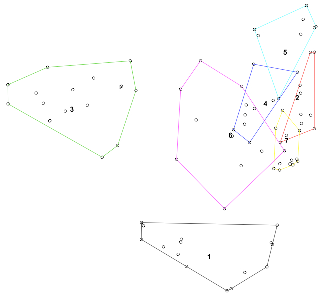
\includegraphics[width=0.75\textwidth]{figures/cluster_map}
\caption{Problem cluster map} \label{fig:cluster_map}
\end{figure}

The complete result data set including all problem clusters and statements can be found in Table \ref{tab:statement_rating}. The following 7 problem clusters covering 82 problem statements were identified:

\begin{compactenum}
	\item[(1)] Access to learning: The cluster covers 15 statements that are mainly related to the challenges of enabling learning in a mobile society. This includes educational problems that are related to flexible learning, including just-in-time learning, equal access to education and learning, and location-based learning. The cluster also covers remote learning and accessibility aspects.
	\item[(2)] Limitations for learning: 9 statements are included in the cluster. The statements cover challenges related to organisational and educational problems of educational institutions that result from different perceptions of the knowledge society in general and mobile technologies specifically among educators and learners. This also includes the problems of using of mobile technologies in formal learning scenarios.
	\item[(3)] Contextual learning: The cluster includes 18 statements that highlight the relation between learning and the context in which the learning takes place. The cluster covers individual aspects of situated learning, learning in context, and learning across contexts. Furthermore environmental aspects are included, such as making use of environmental affordances and a stronger interaction with the environment where the learning takes place.
	\item[(4)] Collaboration: 5 statements are included in the cluster. The statements cover challenges that are related to collaboration, sharing learning resources, and problems related to social interaction, such as difficulties of building a community during learning.
	\item[(5)] Personalisation: The cluster includes 8 statements. The statements range from educational problems with self-directed learning to mass-customisation of learning and reflect the potential of mobile learning to support personal learning processes and engage learners.
	\item[(6)] Orchestrating learning across contexts: 14 statements are included in the cluster, which deals with problems related to current educational practices. The cluster is strongly related to the contextual learning cluster, but focuses more on the organisational aspects that mobile learning can support.
	\item[(7)] Technology and technology adoption: The cluster covers 13 statements %. These statements address 
	addressing challenges related to the technological characteristics of mobile devices and factors of their adoption, including cost-effectiveness, usability, and user-acceptance.
\end{compactenum}

\begin{center}
\footnotesize
\begin{longtable}{l m{8.5cm} c c}
	
	\caption{Rating of problem clusters and statements}\label{tab:statement_rating} \\
 	\toprule
 	\multicolumn{2}{l}{\textit{Problem cluster}} & \multicolumn{2}{c}{\textit{Mean}} \\
 	\multicolumn{2}{l}{\ \textit{Statement}} & \textit{Importance} & \textit{Feasibility} \\
	\midrule
\endfirsthead
 	\multicolumn{2}{l}{\textit{Problem cluster}} & \multicolumn{2}{c}{\textit{Mean}} \\
	\multicolumn{2}{l}{\ \textit{Statement}} & \textit{Importance} & \textit{Feasibility} \\
	\midrule
\endhead
	\multicolumn{4}{r}{(continued)} \\
\endfoot

\endlastfoot

\multicolumn{2}{l}{1. Access to learning} & 4.03 & 3.59 \\
& 17. Access to learning resources and learning opportunities without the restrictions of location, time and cumbersome equipment or facilities & 4.44 & 4.00 \\
& 59. Access to information when and where it is required, through �just-in time� browsing of relevant information, and information push to support learning in context & 4.44 & 3.89 \\
& 41. Easing access to educational opportunities & 4.56 & 3.67 \\
& 25. Mobility of the learner & 4.00 & 4.11 \\
& 79. Including learners from rural areas & 4.22 & 3.89 \\
& 61. Accessibility of information in relevant everyday life and work situations & 4.33 & 3.67 \\
& 9. Learning at anytime & 3.89 & 4.00 \\
& 80. Developing third world countries� education & 4.11 & 3.78 \\
& 8. Learning from any location & 3.89 & 3.78 \\
& 11. Just-in-time information for immediate application & 4.11 & 3.56 \\
& 1. Limited access by some learners in remote locations & 3.67 & 3.89 \\
& 51. Enable learners in classroom settings to have equal access to rich resources and computational tools to support curriculum learning & 3.89 & 3.22 \\
& 78. Including learners with disabilities & 4.33 & 2.78 \\
& 4. Nomads who move from one location to the next while learning & 3.22 & 3.22 \\
& 45. Inequality of access to computers, learning resources and teachers & 3.33 & 2.44 \\
&&&\\
\multicolumn{2}{l}{3. Contextual learning} & 3.92 & 3.60 \\
& 53. Connect learning across contexts, including between formal and informal settings & 4.44 & 3.78 \\
& 16. Ability to discover and experiment in own context & 4.44 & 3.67 \\
& 30. The provision of access to knowledge in the context in which it is applied & 4.56 & 3.56 \\
& 33. Taking education out of classroom settings into meaningful settings & 4.00 & 3.89 \\
& 39. Interacting with your environment to achieve new knowledge from it & 4.22 & 3.67 \\
& 50. Under-utilisation of potentially rich learning resources in heritage sites, art collections and all sorts of other interesting places & 3.56 & 4.22 \\
& 73. Learning in context & 4.00 & 3.78 \\
& 74. Learning across contexts & 4.22 & 3.56 \\
& 58. Using technology to probe or to enrich understanding of the natural environment, and annotating the environment for the benefit of visitors & 3.67 & 4.11 \\
& 29. The design of augmented contexts for development problem to enable collaborative problem solving where learners generate their own �temporal context for development� & 3.89 & 3.78 \\
& 12. Learners cannot learn in context & 3.88 & 3.63 \\
& 57. Making use of affordances of locations to support learning & 3.88 & 3.63 \\
& 55. Enable enquiry-based learning in novel locations, through novel locations, and about  novel locations & 3.89 & 3.44 \\
& 63. Contextualisation of e-learning & 3.67 & 3.56 \\
& 56. Making use of space and environment as a backdrop for engaged spatial learning & 3.67 & 3.22 \\
& 70. The worthwhileness of location-based and contextual mobile learning & 3.56 & 3.33 \\
& 60. Enable learning through distributed conversation across contexts & 3.78 & 2.78 \\
& 3. Insufficient real life experience in the learning process & 3.22 & 3.22 \\
&&&\\
\multicolumn{2}{l}{6. Orchestrating learning across contexts} & 3.59 & 3.28 \\
& 20. Actively participate in learning activities outside of formal educational settings and facilities & 4.44 & 4.11 \\
& 24. Flexibility for the learner & 4.00 & 3.89 \\
& 54. Maintaining continuity of learning across settings, such as between classrooms and museums on school field trips & 4.11 & 3.67 \\
& 62. Documenting real time experiences of learners & 3.89 & 3.78 \\
& 37. Design suitable activities for the mobile learners & 3.89 & 3.67 \\
& 52. Orchestrate new forms of classroom pedagogy that require coordination of individual, small group and whole class activity & 4.00 & 3.33 \\
& 18. Provision of opportunities to contribute to the development/production of learning resources and course content without the restrictions of location, time and cumbersome equipment or facilities & 4.00 & 2.89 \\
& 47. Blinkered, old-fashioned views about education stopping when working lives begin & 3.44 & 3.22 \\
& 40. Anything is a potential learning scenario & 2.88 & 3.50 \\
& 28. Outside in, inside out problem, where cultural practices involving new digital media can be brought into formal learning institution, get enhanced inside the institution and in turn feedback into the digital world at large & 3.22 & 3.00 \\
& 46. Pressured, busy, fragmented, mobile lives leaving little quality time for conventional, place-and-time-dependent education & 3.33 & 2.89 \\
& 64. Transfer of training & 3.44 & 2.56 \\
& 49. Gaps (time lags) between traditionally scheduled learning sessions, limiting achievement, teamwork and collaboration & 3.11 & 2.56 \\
& 31. Refreshing the image and practice of institutional e-learning & 2.56 & 2.89 \\
&&&\\
\multicolumn{2}{l}{5. Personalisation} & 3.46 & 3.13 \\
& 81. Engagement of the learner & 4.44 & 3.56 \\
& 15. Not enough self-directed learning activities while learning & 3.67 & 3.78 \\
& 75. Self-directed learning & 3.89 & 3.11 \\
& 23. Finding new learning strategies that are suitable for the challenges of, and embraces the opportunities of, the knowledge and information age & 3.33 & 3.11 \\
& 43. Students exhibit passivity, boredom, indifference, low attention spans, and fail to complete their studies & 3.44 & 2.78 \\
& 42. The perception that there is a lack of student engagement & 3.11 & 2.89 \\
& 76. Learning with narratives & 2.89 & 3.11 \\
& 77. Mass-customised learning & 2.89 & 2.67 \\
&&&\\
\multicolumn{2}{l}{4. Collaboration} & 3.31 & 3.24 \\
& 19. Provision of opportunities to collaborate, share and publish learning resources and course content without the restrictions of location, time and cumbersome equipment or facilities & 4.33 & 3.33 \\
& 65. Spontaneous collaboration in situated learning & 3.67 & 3.33 \\
& 5. Lack of community building during learning & 3.11 & 3.33 \\
& 7. Not enough collaboration between learners & 2.89 & 3.44 \\
& 10. Learners not able to interact with experts from around the world & 2.56 & 2.78 \\
&&&\\
\multicolumn{2}{l}{7. Technology and technology adoption} & 3.32 & 3.05 \\
& 36. Make use of the affordable technologies that students have access to & 3.78 & 3.78 \\
& 66. Harness the fact that every student in every university owns a sophisticated communications device & 3.89 & 3.67 \\
& 21. Enhance teaching and learning within formal educational settings and facilities through handheld technologies & 3.78 & 3.44 \\
& 72. Get students to use their mobile devices constantly also in education & 3.67 & 3.56 \\
& 34. Helping educational institutions to offer learning aligned to the students� ownership, experience and use of technology & 3.89 & 2.89 \\
& 69. Dealing with small screens and difficult data input & 3.22 & 3.33 \\
& 32. Helping educational institutions understand the increasing and near universal ownership, acceptance and use of mobile devices across society & 3.22 & 3.11 \\
& 27. Cost-effectiveness for the providers of teaching and learning & 3.33 & 2.89 \\
& 26. Cost-effectiveness for the learner & 3.33 & 2.78 \\
& 71. Difficulties to reuse the products & 3.11 & 2.56 \\
& 38. Assess learning experiences to be accountable for the stakeholders & 2.78 & 2.67 \\
& 67. Revolutionise mobile learning, as the iPhone has revolutionised mobile telephony & 2.75 & 2.38 \\
& 68. Make mobile learning a revenue stream for telecommunication companies & 2.44 & 2.56 \\
&&&\\
\multicolumn{2}{l}{2. Limitations for learning} & 3.23 & 2.80 \\
& 22. Finding new teaching methodologies that are suitable for the challenges of, and embraces the opportunities of, the knowledge and information age & 3.44 & 3.22 \\
& 2. Lack of support to young learners, which have the mobile technology & 3.11 & 3.44 \\
& 14. Lack of ICT skills for the twenty-first century & 3.33 & 3.22 \\
& 82. Transformation of traditional education according to the needs of information society & 3.44 & 2.67 \\
& 48. Traditionally ineffective instruction and low learner performance in some subjects & 3.44 & 2.56 \\
& 6. Low motivation of learners who are mobile technology literate & 3.11 & 2.78 \\
& 13. Teachers not comfortable using mobile technology & 3.33 & 2.56 \\
& 44. Rigid assessment systems stifle creativity and innovation & 3.44 & 2.33 \\
& 35. Perceptions of technologically impoverished provision & 2.43 & 2.43 \\

\bottomrule
\end{longtable}
\end{center}

\subsection{Problem Emphasis Analysis}
A detailed analysis of the average rating of the problem statements indicates the experts� opinion about which statements refer to important and feasible educational problems related to mobile learning. Furthermore this analysis also allows estimating the importance and feasibility of the 7 problem clusters as domain concepts. The complete result data set including all problem clusters and statements with attached means can be found in Table \ref{tab:statement_rating}.

Starting with the problem statement emphasis, a statement was considered as important or feasible if the mean was at least 3.5 based on the 5 point Likert-scale rating. An average rating of 3.5 indicates that the experts rated the statement mostly as important or feasible. By taking both rating key dimensions into account the statements can be mapped into four quadrants. Figure \ref{fig:rating_map} shows the quadrants and the mapped statements without identifying the actual statements.

\begin{figure}[!htb]
\centering
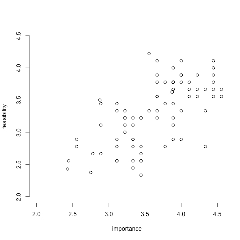
\includegraphics[width=0.9\textwidth]{figures/rating_map}
\caption{Statement rating map} \label{fig:rating_map}
\end{figure}

The first quadrant contains those statements that are relevant on both dimensions, with a high average rating on importance and feasibility. Thus included statements refer to the most relevant educational problems addressed by mobile learning. In the experts� opinion 34 statements are
located in this quadrant. The majority of the statements are related to the clusters �contextual learning� (13 statements), �access to learning� (11statements), and �orchestrating learning across contexts� (5 statements). The highest rated statements within these clusters are also included in the quadrant. The remaining statements are related to the clusters �technology and technology adoption� (3 statements) and �personalisation� (2 statements). The second quadrant contains statements with a high average rating on importance but low average rating on feasibility. The 13 statements in this quadrant can be considered to refer to important educational problems addressed by mobile learning, while sufficient solutions might go beyond the scope of mobile learning. The statements in this cluster are related to the clusters �contextual learning� (4 statements), �access to learning� (2 statements), �collaboration� (2 statements), �orchestrating learning across contexts� (2 statements), and �technology and technology adoption� (2 statements). The remaining statement is related to the �personalisation� cluster.

The third quadrant contains statements with low average ratings on both dimensions. 34 statements fall in this quadrant. These statements are considered to refer to educational problems that are not specifically related to mobile learning in the experts� opinion. The majority of statements in this quadrant are related to the clusters �limitations for learning� (9 statements) and �technology and technology adoption� (8 statements). The remaining statements are related to the clusters �orchestrating learning across contexts� (6 statements), �personalisation� (5 statements), �collaboration� (3 statements), �access to learning� (2 statements), and �contextual learning� (1 statement). The fourth quadrant contains statements with a high average rating on feasibility but low average rating on importance. The quadrant contains only a single statement that refers to a side educational problem to which mobile learning can offer solutions. This statement is related to the �orchestrating learning across contexts� cluster.

\begin{table}[!htb]
\centering
\caption{Highest emphasised problem statements}\label{tab:highest_emphasised}
\footnotesize
\begin{tabular}{m{9cm} c c}
\toprule
                  & \multicolumn{2}{c}{\textit{Mean}} \\
			\textit{Problem statement} & \textit{Importance}	& \textit{Feasibility} \\
\midrule
20. Actively participate in learning activities outside of formal educational settings and facilities. & 4,44 & 4,11 \\
17. Access to learning resources and learning opportunities without the restrictions of location, time and cumbersome equipment or facilities. & 4,44 & 4,00 \\
59. Access to information when and where it is required, through �just in time� browsing of relevant information, and information push to support learning in context. & 4,44 & 3,89 \\
41. Easing access to educational opportunities. & 4,56 & 3,67 \\
53. Connect learning across contexts, including between formal and informal settings. & 4,44 & 3,78 \\
16. Ability to discover and experiment in own context. & 4,44 & 3,67 \\
25. Mobility of the learner. & 4,00 & 4,11 \\
30. The provision of access to knowledge in the context in which it is applied. & 4,56 & 3,56 \\
79. Including learners from rural areas. & 4,22 & 3,89 \\
61. Accessibility of information in relevant everyday life and work situations. & 4,33 & 3,67 \\
\bottomrule
\end{tabular}
\end{table}

Concerning the importance and feasibility of the problem clusters, the average ratings of all problem statements included in a cluster needed to be considered. This analysis revealed that �access to learning� is rated as the most important cluster in the experts� opinion, followed by the clusters dealing with �contextual learning�, �orchestrating learning across contexts�, �personalisation�, �collaboration�, �technology and technology adoption�, and finally �limitations for learning�. Thus in the experts� opinion the accessibility and contextualisation of learning and education are the most important domain concepts that mobile learning can facilitate. The respective clusters also contain the majority of problem statements and as stated the highest rated statements, listed in Table \ref{tab:highest_emphasised}. Regarding the rated feasibility the emphasis is similar. The clusters of �contextual learning� and �access to learning� are rated as the most feasible domain concepts that mobile learning can facilitate, followed by the clusters dealing with �orchestrating learning across contexts�, �collaboration�, �personalisation�, �technology and technology adoption�, and finally �limitations for learning�.

\section{Discussion}
Based on the experts� emphasis the used concept mapping approach identified the most important educational problems that can be addressed by mobile learning. The identified problems are all related to the three main domain concepts �access to learning�, �contextual learning�, and
�orchestrating learning across contexts�, while most of them are related to the concept �access to learning�. This clearly reflects the claim on mobile learning to enable learning across context, facilitating and exploiting the mobility of the learners. The most emphasised issues mainly discuss learning activities and opportunities outside of formal settings, better contextualised and situated learning support, stronger connection between informal and formal settings, and the inclusion of rural and remote learners. Among others these issues indicate the most important current and future use cases for the implementation of mobile learning scenarios. On the other hand the experts considered issues related to technologies and their adoption and usage by teachers, learners and other stakeholders as less important to be addressed by mobile learning. The respective problems are mostly related to the domain concepts �technology and technology adoption� and �limitations for learning�. The emphasis given by the experts does also provide valuable recommendations. Educational institutes and organisations can draw direct conclusions about the core themes of future research agendas and implementation plans out of the study results. To provide an example, the most relevant problem statement within the �Contextual learning� cluster is �Connect learning across contexts, including between formal and informal settings.� The statement is positioned in the first quadrant of the statement rating map shown in Figure \ref{fig:rating_map}, as it got a high average rating on importance and feasibility. In the experts� opinion facilitating learning across contexts is one of the most important challenges in the domain of mobile learning. At the same time there seem to be sufficient solutions to cope with that challenge. The conclusion that can be drawn is that these solution need to be implemented on a short term.

Contrary to this example is the problem statement �Enable learning through distributed conversation across contexts.� covered in the same cluster. The statement is positioned in the second quadrant of the statement rating map with a high average rating on importance but low average rating on feasibility. So in the experts� opinion this challenge is also quite important, but it seems that there are no feasible solutions yet. Examining the statement clarifies this emphasis. To enable a distributed conversation across contexts is related to research in the field of e.g. computer supported cooperative learning. Even if the complex technology mainly coming from the field of mobile and ubiquitous computing is there, it still needs to be utilised in the learning context, which requires additional research efforts also within the field of mobile learning. In addition to the valuable emphasis, the approach also produced a problem cluster map representing the mobile learning domain concepts based on the similarity of the problem statements identified. The main concepts that characterise the educational challenges mobile learning has to cope with are �access to learning�, �contextual learning�, �orchestrating learning across contexts�, �personalisation�, and �collaboration�. The minor domain concepts are �technology and technology adoption� and �limitations for learning�. The produced map can also be used to relate the emerging problem clusters within the overall domain.

The map shows that the clusters �access to learning� and �contextual learning� appear to be independent domain concepts, as they are individually positioned beyond the centre. The other clusters seem to be more closely related and positioned near to the centre. The mapping shows that the �orchestrating learning across contexts� cluster is the central concept within the domain. This indicates that orchestration is the link between the different concepts within the domain of mobile learning. Both the �collaboration� and the �technology and technology adoption� cluster are positioned in close proximity to the central concept, illustrating that the covered problem statements need to be considered when dealing with orchestration and vice versa. The clusters of �personalisation� and �limitations for learning� are positioned a little bit further away from the central concept and thus do not need to be considered equally when orchestrating learning through mobile learning. The same applies for the distant clusters �access to learning� and �contextual learning�.

Focusing on the spatial extend of the single problem clusters, reveals that educational problems covered by the clusters �access to learning�, �contextual learning�, and �orchestrating learning across contexts� are in most cases only loosely related to each other. The mentioned clusters cover a wide problem space. In contrast the other clusters, especially �technology and technology adoption�, cover a relatively narrow problem space with closely related problem statements. On the one hand this underlines that the main domain concepts cover a diversity of educational problems and it might be useful to put more effort on a more finely granulated distinction in order to make further analyses easier to handle. On the other this fact shows that these concepts are still a major point of discussion and there is no agreement on a clear definition related to mobile learning.

\section{Conclusions}
The presented expert concept mapping study provides new insights on mobile learning and the educational problems that underpin the expectations on it. Especially the identified domain concepts contribute to the discussion about the key characteristics of mobile learning, while clarifying the major educational problems that can be addressed by mobile learning. Still the paper outlines only the major findings of the conducted study. The data collected as well as the results obtained from the concept mapping approach allow further profound analyses on single or multiple domain concepts or specific educational issues and their correlation to others. Furthermore the results can also be used to provide guidelines for upcoming discussions on the theoretical and technical developments within the domain of mobile learning. These aspects will be addressed in future work.
%			\clearpage{\pagestyle{empty}\cleardoublepage}


	\part{Mobile authoring of OER for authentic learning scenarios}
		
\chapter{Mobile authoring of OER for authentic learning scenarios}


\vfill
Learning resources are traditionally designed in desktop-based authoring systems where the context is mostly restricted to the learning objective, capturing relevant case characteristics, or virtual situation models. Mobile authoring tools enable learners and teachers to foster universal access to educational resources not only providing channels to share, remix or re-contextualize these, but also capturing the context in-situ and in-time. As a further matter, authoring educational resources in a mobile context is an authentic experience where authors can link learning with their own daily life activities and reflections. The contribution of this chapter is threefold: first, the main barriers for ubiquitous and mobile authoring of educational resources are identified; second, recent research on mobile authoring tools is reviewed, and 10 key shortcomings of current approaches are identified; third, the design of a mobile environment to author educational resources (\em MAT for ARLearn \em) is presented, and the results of an evaluation of usability and hedonic quality are presented.
\vspace{3em}

This chapter is published as: 
Tabuenca, B., Kalz, M., Ternier, S., \& Specht, M. (2014). Mobile authoring of open educational resources for authentic learning scenarios. \em Universal Access in the Information Society\em . Special Issue: The Use of Mobile Technology and Ubiquitous Computing for Universal Access in Online Education), 1�15. doi:10.1007/s10209-014-0391-y

\clearpage

\section{Introduction}
\label{sect:1}
Situated learning \citep{Brown1989} stress the importance of knowledge and skill acquisition in the same context in which they need to be performed; leading also to the concept of communities of practice \citep{Lave1991}. While some educational media simulate real world environments with 3D-visualizations or micro-worlds several authors have stressed the difference between a simulated environment and authentic experiences in the real world \citep{Hummel1993, Tripp1993}. \cite{Rule2006} clusters authentic learning into four themes: (1) real-world problems that engage learners in the work of professionals; (2) inquiry activities that practice thinking skills and metacognition; (3) discourse among a community of learners and (4) student empowerment through choice. The seminal article from  \cite{Herrington2000} identifies a number of design guidelines for situated learning activities like the need to provide authentic tasks and problems as also to support the change of perspectives. 

With the availability of mobile technologies new potentials for the design and creation of authentic and situated learning materials have emerged \citep{Duval2009}. Lombardi and Oblinger \cite{Lombardi2007} identify mobile devices as one of the key technologies to support authentic learning with information access and data collection during field-based investigations. On the one hand, learning support with mobile devices has increased access to advanced learning opportunities. On the other hand, the creation of learning materials in context, and the documentation of authentic learning experiences have been researched. Nevertheless there are still many restrictions for the authoring support of authentic learning resources on different aggregation levels. Several research projects have demonstrated the potential of using mobile and ubiquitous devices to capture contextual information \citep{Zimmermann2005d} and recording real-life experiences \citep{Barreau2007, Hodges2006} but this potential has remained underexploited for the process of mobile authoring of learning resources.

Within this chapter we refer to ''Mobile Authoring'' as the process of content creation on different levels of aggregation by using mobile technologies. \cite{Kinshuk2013} discuss the relevance of mobile authoring when capturing learning where and when it occurs. Additionally, they stress the lack of learner generated content in reusable learning objects authored for e-learning, especially with timely, relevant, and location aware examples. 
This chapter reports about an analysis of existing mobile authoring solutions and the development and evaluation of a new mobile authoring tool  for open educational resources. In the next section we report about related work and discuss shortcomings of current mobile authoring tools. In section 3 we introduce the Mobile Authoring Tool for ARLearn (\em MAT for ARLearn \em) that we have build aiming at authentic learning environments and the related authoring activities as also the shortcomings of analyzed tools. In section 4 we introduce an evaluation of usability and hedonic quality of the \em MAT for ARLearn \em. Section 5 discusses these results and limitations of the work. Last but not least we discuss future research.

\section{Motivation and related work}
\label{sect:2}
Authoring learning resources is currently still a process that is generally conducted in front of a desktop computer making it hard to capture real-life experiences related to the actual learning situation. Most of the current authoring environments are desktop solutions that enable the deployment of the authored learning materials to mobile devices \citep{Perez-Sanagustin2012a, Gruntjens2013, Sampson2012, Gicquel2011, Mathews2010, MartIn2009, Cabada2009, Kim2013}. In this scenario, the user authors an educational resource surrounded by blank walls and situated in front of a computer screen. Authoring educational resources in a mobile context is a more authentic activity that provides access to real-life experiences, which are otherwise not easy to capture. For instance, when creating a learning resource about the architectural design of a building in the physical environment and context in which the building is located, the created learning materials and documentation are expected to be very different from the materials designed on a desktop computer. The creation in-situ and perception of relevant affordances and details is expected to impact the design of instructional materials as also the learning resource selection. 

Remix and re-contexualization are key practices within the field of Open Educational Resources (OER). The combination of authentic learning scenarios and mobile authoring facilitates the connection between real-world locations and digital learning resources. Therefore the reuse and re-contextualization potential can be even larger than in traditional technology-enhanced learning scenarios. Nevertheless, different authors are skeptical on the assimilation and progress of remixing and re-contextualization practices from educators� side.\cite{Amiel2013} concludes that remixing learning resources is still not mainstream in education. \cite{Collis2003} report little success with bringing instructors close to an actual authoring process: ''instructors do not have the time, interest, or skills''. The proliferation of smartphones and the familiarization of new generations with mobile technology are bringing students and educators closer to an authentic and contextualized authoring process and to support reuse and remix of earlier developed resources. 

The work from \cite{Mugwanya2010} reviews mobile learning content authoring tools from 2002 to 2009. The authors categorize these tools according to technology used, pedagogy and usability dimensions. They summarize that the majority of the tools are developed with the goal of being integrated into Learning Management Systems (desktop computer) and stress the need to develop mobile authoring tools that empower users to author content for use in mobile environments. More recently, several authors \citep{Perez-Sanagustin2012a, Gruntjens2013, Sampson2012, Gicquel2011, Mathews2010, MartIn2009, Cabada2009, Kim2013} have proposed solutions for desktop-based authoring of mobile content. These studies report about functionalities like the preparation of routes in maps, the binding of content to QR codes, or language learning content created on mobile devices to be later deployed for mobile learning support. Nevertheless these learning contents are mostly authored in front of a computer screen outside of the real context in which the mobile learning intervention is conducted later.

In contrast to desktop-based authoring, we have conducted a review of existing tools that support the mobile authoring of learning resources. There are different models classifying learning resources according to their granularity \citep{Wagner2002, Duval2003a}. In the following, we will review mobile authoring tools aiming to shed light both on the granularity of mobile generated learning contents, and, what features do mobile authoring tools provide to foster universal access to existing learning resources. 

\subsection{Review in mobile authoring tools}
\label{sect:2_1}
The underlying search was conducted utilizing the online research repositories of the Association for Computing Machinery (ACM), the publisher Springer, Google Scholar, as well as the IEEE Computer Society. The focus on these repositories is reasonable as they cover a sufficiently large number of relevant publications. Within the ACM digital library an advanced search was performed in late January 2014 querying all articles of type journal, proceeding, or transaction that had been published since 2005 when mobile phones became more popular, and matching the keywords ''authoring AND mobile'' as part of the title. The query revealed 8 results whereof 4 were appropriate. As this query did not report enough results, a second search in the full-text matching the keywords ''authoring AND mobile AND learning'' was performed. The query revealed 1051 results where the first 30 occurrences ordered by relevance were selected. These 34 items were filtered by title and/or abstract. The rest of the repositories where analyzed analogously as illustrated in figure \ref{fig:mat_1} The 24 resulting articles were fully analyzed and desktop-based authoring tools were discarded. This review has resulted in eight authentic mobile authoring environments listed in the appendix B ''Authoring tools in mobile context''.
\begin{figure}
	\centering
     \includegraphics[width=0.9\linewidth]{img/mat_fig1}
	\caption{Mobile authoring tools review procedure}
	\label{fig:mat_1} 
\end{figure}
For a more in-depth analysis of the mobile authoring tools identified in the literature review we have compared the different granularity levels that they support in their authored educational resources. As a basis we have used modular content hierarchy from learning objects introduced by \cite{Duval2003a}. The result of this comparison is synthesized in table \ref{tbl:map1}.

\begin{sidewaystable}
  \centering
  \footnotesize
  \caption{Modular Content Hierarchy in mobile authored OER}
  \label{tbl:map1}

\begin{tabular}{lllllll}
\thickhline
\textbf{ } 	
	& \begin{tabular}[c]{@{}l@{}}Raw media \\ data elements \end{tabular}
	& \begin{tabular}[c]{@{}l@{}}Information \\ objects \end{tabular} 	
	& \begin{tabular}[c]{@{}l@{}}Application \\ objects \end{tabular} 
	& \begin{tabular}[c]{@{}l@{}}Aggregate \\ assemblies \end{tabular}  
	& \begin{tabular}[c]{@{}l@{}}Collection \end{tabular} \\ \thickhline
\textit{Mobile Author}	
	& Text 									
	& \begin{tabular}[c]{@{}l@{}}Multiple-choice question, \\ fill in the blanks \end{tabular} 												
	& \begin{tabular}[c]{@{}l@{}}List of questions \end{tabular} 							
	& - 									
	& -         \\ 
\textit{RAFT}			
	& \begin{tabular}[c]{@{}l@{}}Pictures, \\ annotations\end{tabular} 				
	& \begin{tabular}[c]{@{}l@{}}Learning objects \\ (aggregation of pictures, \\ annotations, \\ content metadata, \\ context metadata)	\end{tabular} 
	& - 										
	& - 									
	& -          \\ 
\textit{StoryKit}		
	& \begin{tabular}[c]{@{}l@{}}Pictures, \\ text, \\ drawings, \\ audio files \end{tabular} 
	& \begin{tabular}[c]{@{}l@{}}Page, i.e. text enriched \\ width multimedia \end{tabular} 													
	& \begin{tabular}[c]{@{}l@{}}Book/story, i.e. an \\ aggregation of pages \end{tabular} 		
	& \begin{tabular}[c]{@{}l@{}}Bookshelf, i.e. an \\ aggregation of books \end{tabular} 	
	& -          \\ 
\textit{MPAS}			
	& \begin{tabular}[c]{@{}l@{}}Image, \\ video, \\ text \end{tabular} 					
	& \begin{tabular}[c]{@{}l@{}}Multimedia \\ slides \end{tabular} 																					
	& \begin{tabular}[c]{@{}l@{}}Presentation, \\ aggregation of slides \end{tabular} 		
	& - 									
	& -          \\ 
\textit{MAAIMS}			
	& \begin{tabular}[c]{@{}l@{}}Audio, \\ video, \\ picture \end{tabular} 				
	& Learning object																					
	& - 										
	& - 									
	& -          \\ 
\textit{Quizzer}		
	& Text 									
	& \begin{tabular}[c]{@{}l@{}}Multiple-choice \\ question \end{tabular} 
	& Quiz 										
	& - 									
	& -          \\ 
\textit{mProducer}		
	& \begin{tabular}[c]{@{}l@{}}Video clips \end{tabular} 							
	& \begin{tabular}[c]{@{}l@{}}Learning objects, \\ i.e. aggregation of video \\ and context metadata	\end{tabular} 								
	& \begin{tabular}[c]{@{}l@{}}Stories \\(aggregation of \\ learning objects) \end{tabular}  
	& - 									
	& -          \\ 
\textit{MoVie}			
	& \begin{tabular}[c]{@{}l@{}}Video, \\ text \end{tabular} 							
	& \begin{tabular}[c]{@{}l@{}}Video clip \\objects	\end{tabular} 																			
	& \begin{tabular}[c]{@{}l@{}}Stories \\ (aggregation of videos) \end{tabular} 			
	& - 									
	& -          \\ \hline
\end{tabular}
   
\end{sidewaystable}


Resources that have a low granularity, such us \em raw media \em elements are highly reusable. \em Raw media \em elements include, pictures, text in the form of annotations, audios, video clips, metadata about content, metadata about standard (LOM, SCORM), or metadata about the context (GPS coordinates). \em Aggregate assemblies \em and \em collections \em have higher level of granularity but they are least reusable.

The content taxonomy presented in table \ref{tbl:map1} shows that all mobile authoring tools populate two to four levels of granularity. None of the mobile authoring tools populates the level of \em collection \em in the content taxonomy. This fact indicates that so far, content authored in mobile context is not created to be part of extensive collections, but rather to be integrated in units of lower granularity. An argument for this is the lack of available tools supporting remix of learning contents. 

The analysis of these articles has resulted in the identification of 10 limitations (L1-L10) of mobile authoring tools with regard to universal access of content authored in a mobile context:
\begin{enumerate}
\item Sharing functionality. Authoring tools must feature sharing of authored educational resources in order to foster reuse and facilitate the expansion. Only one of the presented tools allows the sharing of resources created via E-Mail (\em StoryKit\em).
\item Remix support: Remixing allows authors to reuse educational resources and their rearrangement within new application contexts. Only two of the analysed tools provide support to remix resources (\em Quizzer\em and \em Mobile Author\em). While the two tools only allow remix on the \em information object \em level, remix features should be provided on different granularity levels to exploit the full potential of sharing of learning resources.
\item Recontextualization: Recontextualization is the transfer of a learning resource from one context to the other. While related concepts like repurposing \citep{Rensing2005} focus on the change of educational context, for the mobile authoring of learning resources for authentic learning scenarios the re-contextualization from one location to the other is important. The tools \em MAAIMS\em, \em Quizzer\em, \em RAFT\em and Producer support this type of re-contextualization.
\item Editing: Editing of educational resources benefits the adaptation of contents, context, and the rearrangement of the learning objects. Mobile authoring tools should provide mechanisms to support edit of educational resources. Some tools feature edit of the content (\em StoryKit\em and \em Mobile Author\em). MMAIMS feature edit of content metadata, and others feature edit of context metadata (\em Quizzer\em and \em RAFT\em).
\item Search functionality: Mobile authoring tools should provide mechanisms to support allocation of educational resources from repositories \cite{Tabuenca2012c}. Search of educational resources should not only be indexed on the name, description or owner of the educational resource, but also, indexed on the dimensions of the mobile context \citep{Specht2009}, namely, location, time, environment, relation and artefact identification. Hence, mobile devices can facilitate context related search of OER based on the location, time of the day when the resource is useful, or depending on the people surrounding me in a specific moment.
\item Sharing license support: Licensing is an important feature when sharing and reusing mobile content. Recent case study \citep{Amiel2013} implementing remix of OER for language learning highlights the selection of suitable licences as key consideration: ''\em When remixing resources a series of considerations have to take place, which are not necessarily at the forefront in a traditional process of design. First off, one needs to be sure to select resources with more open licenses.\em '' Hence, the license model needs to support this remixing. Creative Commons has the right tools in place to flexibly support remixing of content. None of the presented tools (See appendix C) features any license assignment for authored content. 
\item Learning Object standard support: The implementation of Learning Object Metadata (LOM) standards facilitates content indexing and benefits the integration of OER across Learning Management Systems. Of the analysed tools three support the IMS LOM or SCORM standard: \em MAAIMS\em facilitates the creation of standardized learning objects (IMS Content Packages and standardized learning activities) whereas \em RAFT\em features SCORM.
\item Availability in open app markets: Mobile authoring tools should be available in open app markets as an approach to facilitate universal access to authoring tools. \em StoryKit\em is the only mobile authoring tool available in open markets.
\item Use of sensors: Some of the apps use different sensoring functionalities to support the contextualization and improve the quality of the learning resources. \em Quizzer\em uses the compass to serve content based on the orientation. In authoring mode, \em Quizzer\em records the orientation of the user to contextualize the resource. Moreover, \em Quizzer\em supports tagging of learning resources with the user�s identifier on creation time providing some control on the ownership of the resource. On the other hand, \em mProducer\em uses an accelerometer to measure the excessive amount of camera shaking recording a video, with the aim to filter blurry and unusable recordings. 
\item Interoperability. None of the tools reviewed facilitates the interoperability and exchange of educational resources among different mobile authoring tools.
\end{enumerate}

The above-presented summary shows that there is no ideal mobile authoring tool implementing all the necessary features to exploit universal access. While the availability in open app markets will be targeted at a later stage, we have taken the limitations revealed in the from the scientific literature review into the design of \em MAT for ARLearn \em.

\section{Design}
\label{sect:3}
\em MAT for ARLearn \em has been designed considering the limitations enumerated in the previous section. This tool aims to provide an open environment to facilitate any user (teacher or student) to author, share, edit, remix and recontextualize educational resources to foster universal access. Hereby we describe how \em MAT for ARLearn \em was designed and which of these shortcomings are covered.

\subsection{ARLearn: Cloud-based platform for mobile serious games}
\label{sect:3_1}
The Mobile Authoring Tool has been built upon ARLearn framework, an open source platform for authoring mobile serious games, available under the GNU Lesser GPL license \cite{Ternier2012}. ARLearn is accessible for the community as a cloud based solution where authors can, without cost, create content and deploy this content to mobile devices. Approx. 450 users have used the authoring environment to create games resulting in approx. 600 active games on the platform cloud. As illustrated in table \ref{tbl:map2}, learning resources in ARLearn are classified according to four different granularities in the model of content hierarchy \citep{Duval2003a}. We will further describe these objects providing some examples in the scientific literature where this platform has been used.
\begin{table}[h]
  \centering
  \footnotesize
  \caption{Granularity of learning resources in \em MAT for ARLearn \em}
  \label{tbl:map2}
  
\begin{tabular}{lllllll}
\thickhline
\textbf{ } 	
	& \begin{tabular}[c]{@{}l@{}}Raw media \\ data elements \end{tabular}
	& \begin{tabular}[c]{@{}l@{}}Information \\ objects \end{tabular} 	
	& \begin{tabular}[c]{@{}l@{}}Application \\ objects \end{tabular} 
	& \begin{tabular}[c]{@{}l@{}}Aggregate \\ assemblies \end{tabular}  
	& \begin{tabular}[c]{@{}l@{}}Collection \end{tabular} \\ \thickhline
\begin{tabular}[c]{@{}l@{}}MAT for \\ ARLearn \end{tabular}			
	& \begin{tabular}[c]{@{}l@{}}Pictures, \\ text, \\ drawings, \\ audio files \end{tabular}	
	& \begin{tabular}[c]{@{}l@{}}Audio item, \\ Video item, \\ Multiple-choice, \\ Text item \end{tabular}
	& \begin{tabular}[c]{@{}l@{}}Game\end{tabular}			
	& \begin{tabular}[c]{@{}l@{}}Set of games \end{tabular}	
	& -          \\ \hline
\end{tabular}
\end{table}

ARLearn was extended with an open repository where users can make games open, license it properly and share these with their peers. ARLearn has ben used in several authentic learning scenarios: 
\begin{itemize}
\item Recently, \cite{Schmitz2013} investigated role-playing on helping behavior with a mobile learning game to train basic life support and cardiopulmonary resuscitation. With this game they aimed at improving willingness to help in case of emergency (Figure \ref{fig:mat_2}).
\begin{center}
\begin{figure}[ht]
\centering
	\subfloat[Users had to allocate the defibrillator at the school and use it to save the victim.]{
		\includegraphics[width=0.5\linewidth]{img/mat_fig2a}
		\label{fig:mat_2a}
	}
	\subfloat[Users were instructed on the steps to follow in a cardiac arrest scenario. After the exercise, they were prompted to report the state of the victim.]{
		\includegraphics[width=0.5\linewidth]{img/mat_fig2b}
		\label{fig:mat_2b}
	}	
      \caption{Training cardiopulmonary resuscitation in schools with ARLearn \cite{Schmitz2013}.}
      \label{fig:mat_2}
	
\end{figure}
\end{center}
\item The Mindergie games have been designed and tested at a university campus in the context of an energy conservation pilot \citep{Borner2013a}. The goal of these games is to provide incentive mechanisms to decrease the energy consumption at the workplace. Every week players were given information, tasks and challenges, e.g. a video with hints on how to consume less electricity. 
\item In collaboration with the United Nations Refugee Agency \citep{Ternier2012z}, use cases for crisis situations were developed. These cases feature a social context through role-playing and typically zoom in on crisis situation like a hostage taking scenario. In this game employees are trained on how to react in such a situation. A game here is typically place in 5 phases: notification of the incident, assembling the team, planning, responding and negotiating. During the game players receive message according to their role. The head of office role will get a phone call from a journalist, while the staff welfare member needs to answer a call from a distressed family member.
\end{itemize}
The desktop-based\footnote{ARLearn desktop-based authoring environment. http://streetlearn.appspot.com/
} authoring environment for ARLearn (Figure \ref{fig:mat_3}) features the creation of games, teams, players, roles, items, and the dependencies among them. Moreover, it implements the Creative Commons (CC) licensing policy at the level of games (\em application objects \em) facilitating share and reuse across users. The games presented above are licensed under the CC attribution license. In the next section we describe the design and development of the \em MAT for ARLearn \em.
\begin{figure}
	\centering
     \includegraphics[width=0.9\linewidth]{img/mat_fig3}
	\caption{Desktop authoring environment in ARLearn}
	\label{fig:mat_3} 
\end{figure}

\subsection{\em Mobile Authoring Tool for ARLearn \em}
\label{sect:3_2}
The Mobile Authoring Tool complements the ARLearn desktop-based environment. Hence, a mobile game author can wander around creating items and synchronizing real world artefacts with game content. \em MAT for ARLearn \em has been designed starting a ''Mobile Authoring'' branch \footnote{\em MAT for ARLearn \em source code. https://code.google.com/p/arlearn/source/browse/?name=MobileAuthoring}  from the last release of the open source code available for the ARLearn mobile\footnote{ARLearn in Google Play. https://play.google.com/store/apps/details?id=org.celstec.arlearn2.android} client \citep{Ternier2012}. This procedure has facilitated the reuse of the already existent interfaces to access the backend via RESTful web services and the objects persisted in Google Appengine tables. The design of the tool has been performed adding functionality to the existing client following the next steps: first, we implemented the functionality to create a new game. Until now, it was only possible to create games from the desktop-authoring tool. These games are the containers of items; second, we implemented the functionality to create items so that users can create text items, video item, audio item and multiple-choice item in context recording or taking pictures with the mobile device; third, we perform the scientific literature review and identified the ten limitations for universal access; finally, these shortcomings were analysed and covered as illustrated in appendix C.

The \em MAT for ARLearn \em features three main approaches to foster ubiquitous and universal access to educational resources: 
\begin{enumerate}
\item an author can create and contextualize new content; 
\item an existing game (or an item) can be recontextualized to a new environment; 
\item licensing selection is supported to promote the reuse, revision, remixing, and, redistribution of educational materials as open educational resources (OER).
\end{enumerate}
 
The \em MAT for ARLearn \em features the ''My Games'' view as the starting point. Figure \ref{fig:mat_4a} shows the three games that the user authored for each of the architectural objects he is interested in; Figure \ref{fig:mat_4b} illustrates the ''Game View'' where the user can edit the resource and assign a licensing policy to share it. Clicking on the ''item tab'' (middle one) the user accesses the items that form this game. The author has the option to contextualize the content by binding it to the current coordinates, or by binding it to an existing QR code. Figure \ref{fig:mat_4c} illustrates the case of a user that has created a narrator item (text item) about the Church of St. Peter as an aggregation to the porticos \em Game\em (\em application object \em). As he is located in an authentic environment, for example in front of the church and staring at the portico, the description inspired on the real situation is completely different from the one he would create sited on his desk and watching a picture on the screen. As the user is in a mobile context, he can also contextualize the educational resource to the current location. In this case, the user can contextualize the item with the dimension \em location\em by registering the current coordinates and radius (See top of figure \ref{fig:mat_4c}) clicking on the ''Bind to location button''. The user can also contextualize the item with the dimension \em artifact identifier\em whenever there would be a QR code next to the church. By clicking on the ''Bind to tag'' button, he would scan the code and the educational resource would be attached to that physical object. Next, he can edit the resource to indicate the CC license that should be assigned to the item.
\begin{center}
\begin{figure}[ht]
\centering
	\subfloat["My games" screen lists games created by the author]{
		\includegraphics[width=0.3\linewidth]{img/mat_fig4a}
		\label{fig:mat_4a}
	}
	\subfloat[Authoring games screen]{
		\includegraphics[width=0.3\linewidth]{img/mat_fig4b}
		\label{fig:mat_4b}
	}	
	\subfloat[Contextualization of educational resources]{
		\includegraphics[width=0.3\linewidth]{img/mat_fig4c}
		\label{fig:mat_4c}
	}	
      \caption{Mobile Authoring Tool for ARLearn interface}
      \label{fig:mat_4}
	
\end{figure}
\end{center}
\subsection{OER remix in mobile context}
\label{sect:3_3}
Instead of creating a new resource from scratch the user can search already existing OERs to clone one and aggregate it without making any modification (remix), or, adapting it to the new context by updating any of the dimensions of the mobile context \citep{Specht2009} (recontextualizing). 

The \em MAT for ARLearn \em enables the user to issue a mobile OER search, to assess and to reuse an item in a new context. Users can also extend their game script by reusing a single item rather than reusing a game as a whole. Recontextualizing and remixing needs an infrastructure in place that supports flexible access to content. A search infrastructure must enable searching for content corresponding to different granularities. ARLearn supports searches from two granularities in the modular content hierarchy, namely, \em information objects \em (games), and \em application objects \em (items). Users can author games and items, and make them open access to the community. Figure \ref{fig:mat_5a} illustrates how licences are presented in descendent level of openness according to \citep{Vollmer2013}. Via this infrastructure, the \em MAT for ARLearn \em provides access to search functionality for items as well as for games as a whole when being in a specific context. 
\begin{center}
\begin{figure}[ht]
\centering
	\subfloat[Select level of openness for a new game]{
		\includegraphics[width=0.3\linewidth]{img/mat_fig5a}
		\label{fig:mat_5a}
	}
	\subfloat[Search in already existing items for remix]{
		\includegraphics[width=0.3\linewidth]{img/mat_fig5b}
		\label{fig:mat_5b}
	}	
	\subfloat[Remix and recontextualization of a "text item" with location coordinates or artefact identifier ]{
		\includegraphics[width=0.3\linewidth]{img/mat_fig5c}
		\label{fig:mat_5c}
	}	
      \caption{Remixing and recontextualizing items with the \em MAT for ARLearn \em}
      \label{fig:mat_5}
	
\end{figure}
\end{center}
Figures \ref{fig:mat_5b} and \ref{fig:mat_5c} illustrate a case remixing and recontextualizing educational resources in a mobile context:
\begin{itemize}
\item Remixing. The user is interested in including a video on the architecture of the Cathedral in Aachen. Instead of creating it, he uses the search tool (Figure \ref{fig:mat_5b}) to look for already existent educational resources. He finds an educational resource from a guided tour that somebody had previously shared. He clones the item and aggregates it as a whole into the game, without modifying it (Figure \ref{fig:mat_5c}).
\item Recontextualization. In this case, the user is interested in including a multiple-choice-question to assess knowledge on medieval porticos. Instead of creating it he uses the search tool (Figure \ref{fig:mat_5b}) to look for already existent assessments on porticos. He finds one that was previously bound to the porticos at the Cathedral of Cologne. He clones the item, modifies the context by binding it to current coordinates and radius (Figure \ref{fig:mat_4c}), or a QR tag (Figure \ref{fig:mat_5c}), and aggregates it into the game. 
\end{itemize}
The \em MAT for ARLearn \em features a new quality for recontextualization. This tool provides mechanisms to recontextualize educational resources in different dimensions like ''location'' and ''artifact identifier'' via sensors. Making content appear when the user enters a zone, is an example of binding the content to location using the GPS of the device. QR codes enable the identification of real world artifacts using the camera and the QR reader of the device. Binding content to a QR code is thus a means to synchronize them with the artifact. Image recognition, or, text recognition tags are similar approaches to recontextualize OER with the artifact identifier dimension. ARLearn allows for tagging artifacts with Radio Frequency Identification (RFID) tags or bar codes (QR, EAN-13) as an easy and open procedure to enrich physical spaces with machine-readable tags.

\subsection{OER licensing policy definition}
\label{sect:3_4}
Creative Commons fosters share and reuse of OER. An easy to use and legally interoperable license is a critical component for the OER movement \citep{Atkins2007}. Table \ref{tbl:map3} illustrates how OER can be legally remixed with other OER. It is important to highlight that when implementing cross-license remixing, only one third of CC�s own licenses are compatible.

\begin{table}[h]
  \centering
  \small
  \caption{Remix compatibility according to spectrum of freedom in Creative Commons licenses}
  \label{tbl:map3}

\begin{tabular}{rccccccc
>{\columncolor[HTML]{EFEFEF}}l }
\multicolumn{1}{l}{\cellcolor[HTML]{EFEFEF}\textbf{Most Open}}                          & \multicolumn{1}{l}{\begin{turn}{90}PD\end{turn}}                       & \multicolumn{1}{l}{\begin{turn}{90}BY\end{turn}}                       & \multicolumn{1}{l}{\begin{turn}{90}BY-SA\end{turn}}                    & \multicolumn{1}{l}{\begin{turn}{90}BY-ND\end{turn}}                    & \multicolumn{1}{l}{\begin{turn}{90}BY-NC\end{turn}}                    & \multicolumn{1}{l}{\begin{turn}{90}BY-NC-SA\end{turn}}                 & \multicolumn{1}{l}{\begin{turn}{90}BY-NC-ND\end{turn}}                 & \multicolumn{1}{c}{\cellcolor[HTML]{EFEFEF}\textbf{\begin{turn}{90}Least Open\end{turn}}} \\
PD                                                              & $\surd$                                      & $\surd$                                      & $\surd$                                      & $\surd$                                      & $\surd$                                      & $\surd$                                      & $\surd$                                      &                                                                 \\
BY                                                              &                                              & $\surd$                                      & $\surd$                                      & $\surd$                                      & $\surd$                                      & $\surd$                                      & $\surd$                                      &                                                                 \\
BY-SA                                                           &                                              &                                              & $\surd$                                      &                                              &                                              &                                              &                                              &                                                                 \\
BY-ND                                                           &                                              &                                              &                                              & $\surd$                                      &                                              &                                              & $\surd$                                      &                                                                 \\
BY-NC                                                           &                                              &                                              &                                              &                                              & $\surd$                                      & $\surd$                                      & $\surd$                                      &                                                                 \\
BY-NC-SA                                                        &                                              &                                              &                                              &                                              &                                              & $\surd$                                      &                                              &                                                                 \\
BY-NC-ND                                                        &                                              &                                              &                                              &                                              &                                              &                                              & $\surd$                                      &                                                                 \\
\multicolumn{1}{l}{\cellcolor[HTML]{EFEFEF}\textbf{Least open}} & \multicolumn{1}{l}{\cellcolor[HTML]{EFEFEF}} & \multicolumn{1}{l}{\cellcolor[HTML]{EFEFEF}} & \multicolumn{1}{l}{\cellcolor[HTML]{EFEFEF}} & \multicolumn{1}{l}{\cellcolor[HTML]{EFEFEF}} & \multicolumn{1}{l}{\cellcolor[HTML]{EFEFEF}} & \multicolumn{1}{l}{\cellcolor[HTML]{EFEFEF}} & \multicolumn{1}{l}{\cellcolor[HTML]{EFEFEF}} &                                                                
\end{tabular}

\end{table}

When a game is created with open licence (different than CC-BY-NPD), all items will inherit this license by default. Nevertheless, licences from items can be consistently updated whenever both game and item licences are compatible. If a game specifies a No Derivatives (ND) licensing attribute, its items will not be searchable or reusable. In such case only the game as a whole can be reused. When a user reuses an existing game, the original author will be appropriately credited. A user that reuses a ShareAlike (SA) licensed game will not be able to restrict the access rights. Furthermore, an interesting situation occurs when a user reuses an item: if a user reuses a video that should be SA, the entire game becomes SA. 

\section{Evaluation}
\label{sect:4}
Authoring contents with mobile technologies must be accomplished in an efficient and intuitive way that facilitates the user to create new resources in any specific context. Quantifying the usability of the Mobile Authoring Tool is key to determine how suited is the system to be used across contexts. We have conducted an evaluation of usability and hedonic quality of the \em MAT for ARLearn \em tool. In this section we present the methods, instruments and results of the evaluation.

\subsection{Method and participants}
\label{sect:4_1}
This study was conducted in February 2014 at the Open University of The Netherlands. An invitation was distributed via E-Mail with the aim to recruit participants for an experiment within the Technology Enhanced Learning Lab. Seven employees (AVG age = 34, male, all smartphone owers) voluntarily reacted to the invitation. The experiment was performed during one day with a time limitation of 30 minutes per participant and the participation was not rewarded.

In the instruction phase the participants were introduced the concept of ''mobile authoring'' as the process of producing content by building up materials in the authentic context where these artifacts or persons are normally interacting, in order to build learning ecologies. They were prompted to create a welcome game for new employees at the lab that should describe relevant resources at the workplace like technological equipment (scanner, heating control, fax, photocopier, WI-FI, coffee machine, etc.), people (room-mates, project colleague, etc.), and descriptions on how to get acquainted with the work at the institute. We suggested producing resources with a specific purpose so they can be further reused by forthcoming participants (e.g. a guide for new employees, guide of labour risks at your workplace, measures for energy saving at workplace, etc.). 

As illustrated in figure \ref{fig:mat_7}, the mobile authoring phase comprised the creation of one text item, one video item, one audio item, and one multiple-choice question that people could use to collect the assessments for these artifacts (e.g. quality of the printer, strength of the WI-FI signal in specific meeting rooms), and remix one item by choosing it from the list of shared items and edit it for reuse. Participants are asked to contextualize items by binding them to tagged artifacts (QR codes) or coordinates (GPS location). Likewise, participants were able to recontextualize items by remixing already tagged artifacts and editing the information of the context. In the last phase, participants were prompted to fill in a usability questionnaire and provide qualitative input about the hedonic quality of the tool.
\begin{figure}
	\centering
     \includegraphics[width=0.9\linewidth]{img/mat_fig7}
	\caption{Flow of the experiment. UML-State diagram}
	\label{fig:mat_7} 
\end{figure}

\subsection{Instruments}
\label{sect:4_2}
The material for the study consisted in a first introduction of the experiment with a set of instructions to be read on paper, an Android smartphone (Sony XPeria S) with the \em MAT for ARLearn \em installed in it, and a desktop computer for accessing the post-questionnaire.

The System Usability Scale (SUS) was used for the evaluation of the usability \cite{Brooke1996}. The SUS scale consists of 10 questions with a five-point Likert scale, where item directions are changed in each question. The results of the survey were recorded in an online questionnaire. Based on the current literature, a SUS score above 68 (SD:12,5) is rated as usability score above average. This analysis have followed the recommendations from \cite{Sauro2011} so that the results can be mapped and benchmarked against 446 previous studies and 5000 individual responses.

\cite{Hassenzahl2001} has discussed the limitations of taking only into account usability and proposed in addition to take into account the ''hedonic quality'' of an interface. Hedonic quality is defined as the non-task related quality dimensions like ''accessibility'' or ''originality''. We employed the Reactiondeck toolkit developed by \cite{Benedek2002} to assess these aspects. These product reaction cards have been transferred to a digital version and published as Reactiondeck toolkit \citep{Storm2012}. Thus, participants were asked to select 6 product reaction cards that describe the emotional appeal of the mobile applications best and provide arguments on the selection (See Figure \ref{fig:mat_8}). After choosing the cards, users were invited to argue in an open text box why did they selected that card.
\begin{figure}
	\centering
     \includegraphics[width=0.9\linewidth]{img/mat_fig8}
	\caption{Evaluation of hedonic quality with the Reactiondeck \cite{Storm2012}.}
	\label{fig:mat_8} 
\end{figure}

\section{Results}
\label{sect:5}
Participants created (audio, text, video) resources to explain how to extend notebook�s screen to a bigger display, how to setup the fax, how to get cold sparkling water from the coffee machine, how to use the badge to access different buildings or how to play a demo in the eye-tracker of the lab (Figure \ref{fig:mat_5b}). Participants created multiple-choice questions to rate the quality of the printer, how clean is the lab, or the quality of the coffee machine. Participants remixed items like the photocopier instructions that only differed in the password depending on the building within the campus, or scanner instructions that differed in some steps depending on the brand of the device.

\subsection{Usability}
\label{sect:5_1}
The evaluation of the usability shows that \em MAT for ARLearn \em has a mean score of 80 (SD = 7.2), which is remarkably above average (SUS more than 68). Items 4 and 10 from the questionnaire were taken as subscale for learnability. Average learnability score was 17,81 where two participants (user 2 and 8) rated slightly below average. Items 1, 2, 3, 5, 6, 7, 8, 9 contribute to the construct usability where average score was 62,81 and only one participant rated below average (user 3).
\begin{figure}
	\centering
     \includegraphics[width=0.9\linewidth]{img/mat_fig9}
	\caption{Evaluation of Usability and Learnability with the System Usability Scale (SUS) \cite{Brooke1996}.}
	\label{fig:mat_9} 
\end{figure}

\subsection{Hedonic quality}
\label{sect:5_2}
The Hedonic quality evaluation harvests adjectives that define the interface and usability of the tool considered in terms of pleasant (or unpleasant) sensations. Figure \ref{fig:mat_10} illustrates which were the most selected adjectives to determine the hedonic quality of the \em MAT for ARLearn\em . ''Organized'' and ''Usable'' were the most voted adjectives by the participants (n=4). E.g. regarding the organization users argued: ''\em The distribution of items, icons and buttons within the screen is consistent\em '', ''\em The interface is clear, and there are not useless elements on the screen. All of them are self-explanatory\em ''. These adjectives highlight a suitable distribution not only of the functionality across screens, but also of the elements (buttons, images, text boxes, etc.) used within the screens. Regarding the ''usability'' participants argued: ''\em The tool is intuitive and I feel confortable using it\em '', ''\em All choices for authoring are self-explained thus the tool is easy to use\em ''. Three participants selected ''Easy-to-use'' and two participants selected ''accessibility'' arguing ''\em It is easy to get access to configuration procedures of artefacts through mobile devices\em ''. These adjectives reveal an appropriate usability of the tool since participants could intuitively navigate without instruction and based on what they felt to be necessary. 

One participant highlighted the importance of providing open access to authored resources ''\em It is nice to share knowledge with others\em ''. This comment recognises the benefits of openly sharing knowledge as a way of actively promoting innovation, developing educational capacity and speeding up the processes by which researchers and academics review and build on each other�s work. On the other hand, the willingness of users to share their identify tagging authored educational resources with a suitable licence keeps being a controversy. In fact, two-participants reported their reluctance selecting the card for ''not-secure'' and arguing that ''\em The identity of the user might be in danger when sharing resources\em '', ''\em I am not happy sharing my identity when sharing content\em ''. 
\begin{figure}
	\centering
     \includegraphics[width=0.9\linewidth]{img/mat_fig10}
	\caption{Tag cloud visualization for the measure of hedonic quality.}
	\label{fig:mat_10} 
\end{figure}

\section{Discussion and Conclusions}
\label{sect:6}
The chapter has introduced the lack of authenticity in situated learning scenarios of desktop-based authoring systems in contrast to mobile-based authoring systems where resources can be enriched with users� context \citep{Specht2009}, \em namely \em , \em  location\em, \em time\em, \em environment\em, \em relation\em and \em artefact identification\em. This chapter proposes the use of mobile authoring tools not only as a solution to cover this gap, but also to foster universal access to educational resources. The review of scientific literature has revealed eight mobile tools for authoring of educational resources in a mobile context. These resources have been classified according to the Modular Content Hierarchy model \citep{Duval2003a}  (table \ref{tbl:map1}) with the aim to identify the grain of their authored resources towards the definition and the levels they can aggregate. Based on an analysis of these tools we have recognized ten shortcomings (L1 to L10) mobile authoring tools should cope to foster universal access to educational resources authored in a mobile context (see appendix C). 

These features have influenced the design and development of the \em MAT for ARLearn \em tool. In contrast to the existing standalone tools reviewed in this chapter, \em MAT for ARLearn \em has a scripting environment for mobile serious games for learning in the background. \em MAT for ARLearn \em has extended the state-of-art of authoring tools featuring 7 of the 10 limitations concluded in the literature review, namely,  (L1) share, (L2) remix, (L3) recontext, (L4) edit, (L5) search, (L6) licence support, (L9) use of sensors. This tool features searching, editing and sharing of learning OERs via Creative Commons licences facilitating the remix of contents. Moreover, \em MAT for ARLearn \em features the creation and contextualization of educational resources on two of the dimensions of the mobile context \citep{Specht2009}:
\begin{itemize}
\item Location. Users can bind authored resources to locations. E.g. an audio recording on a specific architecture linked to the geographical coordinates (longitude, latitude, radius) of a church (Figure \ref{fig:mat_4c}). Location coordinates can be obtained via GPS sensors in mobile phones.
\item Artefact identity. Users can bind authored resources to tags attached to physical objects. E.g. text instructions on how to use a photocopier linked to a QR code (Figure \ref{fig:mat_5c}). Barcodes or NFC tags are instances of artefact identifiers accessible via sensors in mobile devices.
\end{itemize}
Results of a usability evaluation have confirmed that the tool has usability above average and that users understand the functionalities of the tool. These findings are reinforced by the hedonic quality evaluation conducted. We believe that mobile authoring tools that allow for content sharing under open content licensed will be a key enabler for building an ecology of digital learning resources which are freely available in the direct environment of learners and which can be re-used, adapted and recontextualized. Moreover, both the measure of �usability� and �hedonic quality� presented in this chapter, can be taken as a reference for forthcoming developments of authoring tools serving as a base for future quantified and qualified comparisons. 

The review of authoring tools presented in this chapter is limited to systems found in scientific literature. This research should be extended to the ones existing in open app markets (Android, iOS, Windows, Blackberry, etc.). 
\em MAT for ARLearn \em is currently in BETA version and will be released in the Google Play market as one more feature within the framework (L8). 

In future research, we will develop and evaluate further features to (re)contextualize learning contents with the pending dimensions of the mobile context \citep{Specht2009}: time (e.g. a video recording on an specific historic which is only made available to appear on anniversary dates); relation (e.g. an educational resource that is only made available to appear when all the members of a group are together); environment (e.g. ''\em whenever the temperature is higher than 40 degrees, play an audio item on measures to prevent dehydration\em '').




			\clearpage{\pagestyle{empty}\cleardoublepage}	

	\part{Stop and Think: Exploring Mobile Notifications to Foster Reflective Practice on Meta-Learning}
		\chapter{Stop and think: Exploring mobile notifications to foster reflective practice on meta-learning} 

\vfill
This chapter explores the effectiveness of mobile notifications to foster reflection on meta-learning by presenting the results of two studies: 1) a formative study with 37 secondary school students offering a daily reflection and reporting exercise about their learning experience during the day; 2) an experiment involving 60 adults to read an eBook on energy-efficient driving for one hour. During that time, the participants received mobile notifications inviting them to reflect in-action. On the one hand the results from the first study show that students do not have a habit of seeing themselves as learners and developing a \textit{�professional�} awareness about their daily activity at work/school. On the other hand the second study explores the effects of different notification types on knowledge gain and motivation. Results envision a higher knowledge gain and motivation for the group assigned with the least complex interactions with mobile devices during the reflection exercise.
\vspace{3em}

This chapter is published as: 
Tabuenca, B., Kalz, M., Ternier, S., \& Specht, M. (2014). Stop and think: Exploring mobile notifications to foster reflective practice on meta-learning. \em IEEE Transactions on Learning Technologies\em . Special Issue on Seamless, Ubiquitous, and Contextual Learning. 1�12. doi:10.1109/TLT.2014.2383611

\clearpage

\section{Introduction}

Based on current trends \citep{Publishing2011}, it is estimated that 84 percent of today�s young people in OECD countries will complete upper secondary education over their lifetimes. This period consolidates students� basic skills and knowledge towards a successful transition to either an academic or a vocational pathway. While graduation rates give an indication of the extent to which education systems are succeeding in preparing students to meet the labour market�s minimum requirements, they do not capture how the students have developed an identity as learners. The acquisition of such an identity, and the associated reflective transversal skills, grow in importance in a \textit{�lifelong learning society�} \citep{EuropeanComission2005}. In the formal education system it is a challenge to find ways to provide students with opportunities to mentally evoke what they have learned throughout the day, so that this experience can be turned into a deliberate object of attention and reflection.

\textit{Learning to learn} and \textit{Digital competence} are highlighted as two of the eight key competences for lifelong learning in the European Reference Framework \citep{EuropeanCommission2007}. The proliferation of wirelessly-networked technologies facilitates the scaffolding of \textit{seamless learning spaces} \citep{Chan2006} as an approach for continuing learning experiences across different scenarios, and emerging from the availability of one device or more per person. \cite{Biggs1985} defines meta-learning as an awareness and understanding of the phenomenon of learning itself as opposed to subject knowledge. Hereby we conceive meta-learning activities as the increase of knowledge and motivation on learning when triggered by introspective episodes of reflection on user�s own learning. Hence the present chapter explores different instantiations of notifications received on mobile devices with the aim to foster reflective practice for meta-learning measuring the variations in dependent variables of knowledge and intrinsic motivation.

Reflection is the practice to become aware of an implicit knowledge base and to learn from experience \citep{Schon1983}. Sch\"on coined the terms \textit{reflection in-action} as the reflective practice performed while doing an activity to optimize the immediately following action, and \textit{reflection on-action} as the reflective practice performed when the activity has finished in order to review, analyse, and evaluate the situation and gain insight for improved practice in the future.

Previous work on reflection amplifiers in-action suggests that regular changes between meta-cognitive and content focus, lead to more awareness and self-regulative competences in the learning process \citep{Bannert2009,Verpoorten2012}. Reflection amplifiers are compact and well-considered prompting approaches that offer learners structured opportunities to examine and evaluate their own learning \citep{Verpoorten2009}. They are presented as structured and repeated introspective episodes, offered in the course of action and meant to make learning visible. The effectiveness of mobile notifications to foster reflective practice on learning (reflection on-action) has not been explored yet. Recent research suggests that mobile notifications by students produce distracting effects \citep{Fried2008,Kraushaar2010}. Nonetheless, notifications received on mobile devices have also resulted in a positive impact, suggesting that the intervention is able to improve students� self-regulated learning effort. The study from \cite{Goh2012a} used persuasive SMS interventions on undergraduate students for 12 weeks, showing that students who received SMS intervention performed better than students who did not receive SMS intervention. \cite{Cavus2009} investigated the effects in knowledge and enjoyment of sending SMSs with English vocabulary to 45 first-year undergraduate students concluding that students enjoyed and learned new words with the help of their mobile phones. Similar, \cite{Thornton2005} used more elaborated notifications in the form of emails to teach English vocabulary lessons to university students concluding that students that received the mobile email learned more than those that received web-based email. \cite{Uzunboylu2009} implemented multimedia messages to increase awareness on environmental concerns. Measures of enjoyment, knowledge or awareness have been the focus of previous research.

This chapter presents two studies evaluating approaches to stimulate learners� capacity of reflection by making \textit{what they learn} a deliberate object of attention \citep{Watkins2001}. The research is embedded into a larger project focusing on mobile support for lifelong learning \citep{Tabuenca2013,TabuencaCAA2014,Tabuenca2014d}. More specifically, in this work we have focused on the use of notifications instantiated in mobile devices for lifelong learning support. Research on notification and prompting for reflection suggest different strategies for reflection on-action and in-action. This work advances the research on mobile notifications and reflective practice presenting two studies:
\begin{itemize}
\item A formative study aimed to reflect on-action. This study was carried out during two school days and two days off, in which 37 college pupils were prompted via mobile SMS notification for a daily reflection and reporting exercise about how they have learned during the day (intensity and channels).
\item An experimental study aimed to reflect in-action. In this study, 60 university employees were invited to read an eBook on energy-efficient driving. During that time, they were prompted via mobile notifications to reflect and report on what they had learned.
\end{itemize}
The following sections introduce both experiments by mapping the goal of the research to existing gaps that need to be covered. The results are discussed and important research questions are raised.

\subsection{How to design mobile notifications for student reflection support}
The first study presented in this chapter transposes \textit{reflection amplifiers} \citep{Verpoorten2009} to mobile (meta-)learning, after-school setting and analytical scrutiny onto one�s learning day.  In this study, students have been assigned to reflect about the learning affordances offered to them throughout the day. Three main research questions have guided this formative study:
\begin{enumerate}
\item How will students respond to invitations to reflect on personal learning sent on their own device and outside the school hours (participation)?
\item What insight does this sampling of experience bring regarding how learning takes place in students� today common life (channels of learning and perceived intensity)?
\item What effects of these structured episodes of introspective reflection can be pinpointed on dimensions of learning (familiarity, appreciation, perceived learning, account of the learning experience)?
\end{enumerate}
In a second experiment, variations of mobile notifications prompting users to reflect in-action have been explored, and the effects on knowledge gain and motivation have been quantified.
On the one hand thinking aloud \citep{Nielsen2002} and sampling of experiences \citep{Hektner2007} have been pinpointed as effective approaches to foster reflective practice on learning. The majority of the studies sampling experiences with educational implications have involved children and adolescents \citep{Hektner2007}. Hence, this experiment has been performed with adults. On the other hand \cite{Wong2011d} identify ten seams by which learning experiences are disrupted and for which mobile seamless learning technology has to find new solutions. One of them is \textit{�the combined use of multiple device types�}. In many cases it is presumed that learners interact only through a single channel or device. However, the technological framing can vary from single device interaction to the presence of multiple devices with different characteristics and capabilities that are used simultaneously. Likewise, the proliferation of tagged objects and the incorporation of tag readers (i.e.QR codes, NFC tags) to mobile devices are facilitating the exchange of educational content across devices.
This experiment explores variations of mobile notifications for adults sent with the aim to foster reflective practice in-action while accomplishing a learning activity. This setup contemplates the combined use of multiple devices for learning and has been guided on three main research questions:
\begin{enumerate}
\setcounter{enumi}{3}
\item How  students perceive asynchronous notifications in contrast to user-triggered notifications prompting reflection in-action, and what effects on knowledge and motivation can be highlighted?
\item What insights can be gained when using mobile notifications prompting the student to actively externalize an exercise of reflection in-action, and what effects on knowledge and motivation can be highlighted?
\item Which reflection cues are provoked by the spontaneous collection of learning objects with mobile devices, and what effects on knowledge and motivation can be highlighted?
\end{enumerate}

\section{Study 1: Embedding reflection in everyday activity via SMS notifications}
\subsection{Method}
\subsubsection{Participants}
This study enrolled 37 college students (mean age = 17 years old, 37\% female, 63\% male). An iTunes voucher of 15 EUR rewarded their participation in the experiment. The voucher was delivered to students that completed both the pre-questionnaire and the post-questionnaire.

\subsubsection{Materials}
The formative study aimed to attract every student to perform the reflection exercise, no matter which mobile device they were using. It was decided to use SMSs notifications to make them all aware when the personal response system was ready to accomplish the reflection exercise. Participants that reported to own a phone with Internet connection (67\%) could follow the link in the SMS (See Figure \ref{fig:notif_1}a) to directly navigate within the personal response system. Participants without mobile Internet connection (33\%) used alternative devices (personal computers or tablets) to log in via browser navigation of the same URL. The students' personal response system\footnote{Socrative. Multiplatform audience response system. http://www.socrative.com/}  selected for this formative study features multiple-choice questions (Figure \ref{fig:notif_1}bc), short text answers, and long text answers. This platform can be accessed from smartphones, tablets, laptops and personal computers. Materials, experimental design and partial results of this study were reported earlier  \citep{Tabuenca2012d}. The current chapter provides additional data (Table \ref{tbl:notif_table2} and dropouts examination) extending the analysis of these results and its implications.
\begin{center}
\begin{figure}[ht]
\centering
	\subfloat[Daily SMS received by students]{
		\includegraphics[width=0.3\linewidth]{img/notif_fig1a}
		\label{fig:notif_1a}
	}
	\subfloat[Personal response system: \em What was your main learning channel today? \em]{
		\includegraphics[width=0.3\linewidth]{img/notif_fig1b}
		\label{fig:notif_1b}
	}	
	\subfloat[Personal response system: \em How intense was your learning day? \em]{
		\includegraphics[width=0.3\linewidth]{img/notif_fig1c}
		\label{fig:notif_1c}
	}	
      \caption{Formative study. Notifications fostering reflective practice on-action}
      \label{fig:notif_1}
\end{figure}
\end{center}
\subsubsection{Design}
The design of this study considered the same treatment for all the participants. Regarding the independent variables, this formative study considered three measures:
\begin{itemize}
\item A pre-questionnaire gathered perception of students about the intensity of their learning week and the main channel they use for learning. 
\item A daily mobile questionnaire was the reflection amplifier of the study. It comprised one question about the perceived intensity of the learning day (Figure \ref{fig:notif_1c}) and one question about the main channel of learning used during the day (Figure \ref{fig:notif_1b}).
\item A post-questionnaire left active during one week served to explore the effects of introspective episodes of reflection on meta-learning defined as awareness and understanding of the phenomenon of learning itself \citep{Biggs1985}. Hence, participants were prompted to reflect and report on \textit{�What is learning?�}, their familiarity with reflective practice, their appreciation of the reflective practice, and their description of the learning experience. Additionally, they were asked to provide an account on their learning channels, and the intensity of their learning during the days of the experiment. The high rate of dropouts motivated the adaptation of a post-questionnaire with the intention to explore the reasons why some students did not take part in the daily reflective exercise.
\end{itemize}

\subsubsection{Procedure}
The study took place during an �experiment day� which offered students to discover the work of the Learning Innovation Lab (the authors� workplace) through the participation in empirical experiments. At the end of the day, a presentation provided an overview of mobile technologies for learning. Afterwards, the corresponding author introduced the participants to the exercise to be done in the next 4 days. The formative study was introduced to students as a reflection exercise in which they were supported to improve their awareness of their daily activity as learners. The famous speech of Steve Jobs at the end of the year session at Stanford University\footnote{Jobs, S. (2005). Commencement address delivered at Stanford University, June 12, 2005. Stanford Report. Available in http://www.youtube.com/watch?v=xoUfvIb-9U4}  was used as a stance on the importance to step back and consciously attend to one�s own life and personal identity, here as a learner. The experiment required using both a SMS broadcasting system that would alert them about the reflection moment of the day, and a student response system where they should answer the questions they would be asked. The students completed the pre-questionnaire and a demo from both the SMS functionality and the student response system was performed.

The daily reflection exercise was performed during 4 consecutive days after the presentation of the experiment. This setup was designed to evenly distribute the reflection exercises across two days at school (Thursday to Friday) and two days out of school (Saturday to Sunday). It allowed to encompass the awareness and reflection on both formal and informal learning and to provide contrast to the descriptions of the learning experience. An SMS was sent to students every day at 8 pm alerting them that the student response system was ready to receive answers with their reflections. Students that had smartphone with Internet connection could click the link and perform the reflection exercise within the platform directly on their smartphone device. The virtual classroom enabled the teacher monitor how many students were performing the activity in real time. Finally, the students received an email inviting them to complete the post-questionnaire.

\begin{figure}
     \centering
     \includegraphics[width=0.7\linewidth]{img/notif_fig2}
     \caption{Evaluation of the participation in the formative study}
     \label{fig:notif_2}
\end{figure}

\subsection{Results}
\subsubsection{Participation}
The first research question aimed to explore student�s willingness to participate in a reflection exercise and to what extent students would react actively to regular invitations to reflect on personal learning experiences sent on their own device and outside the school hours. The decrease in participation (Figure \ref{fig:notif_2}) was quite visible in each of the four iterations of the daily questionnaire (mean 2\%), but was not as severe as the dropout rate from the pre-questionnaire to the mere entrance in the daily exercise (48\%). The 29 recorded post-questionnaires comprised both the participative (56\% [n=16]) and the dropouts (44\% [n=13]). In this study, we refer to dropouts as the students that voluntarily decided not to take part in the daily reflection exercise (Day 1 to 4). Dropout students had the chance to get the reward (iTunes voucher) whenever they completed the post-questionnaire for dropouts.

Main invoked reasons for dropouts (n=13) were for 46\% \textit{�I did not receive any SMS�} and 38\% \textit{�I had no Internet connection at that moment�}. No respondent selected lack of interest, boredom of the intrusive character of the experiment as justifications for not participation. The SMS monitor tool confirmed the failures delivering the messages: an average of 15\% of the SMS were not delivered, a large majority thereof caused by a wrong phone number given by the students right from the start of the experiment. Additionally, the monitoring tool for teachers of the student response system displayed how many students were connected to the platform filling-out the questionnaire in every moment. From these observations, it can be concluded that the majority of the students reported their answers in the same moment they received the SMS.

\subsubsection{Intensity of the learning day and channels used}
The second research question aimed to gain insights on what this sampling of experience brings regarding how learning takes place in students� life focusing on their channels of learning (Figure \ref{fig:notif_1b}). Table \ref{tbl:notif_table1} summarizes the answers given by students both in the pre/post-questionnaires and in the daily reflection exercises. School and Internet were reported as the most important sources of learning.

The post-questionnaire shows that the majority of the participants in the daily reflective exercise reported the school as the main channel of learning during those days. Nevertheless, the majority of the dropouts identified Internet as the main leaning channel.
\begin{table}[h]
  \centering
  \footnotesize
  \caption{Main channels of learning}
  \label{tbl:notif_table1}
  
\begin{tabular}{llllllll}
\thickhline
\textbf{ }								
	& \multicolumn{1}{c}{\textbf{School}}	
	& \multicolumn{1}{c}{\textbf{Internet}}
	& \multicolumn{1}{c}{\textbf{Conversations}}
	& \multicolumn{1}{c}{\textbf{Leisure}}
	& \multicolumn{1}{r}{\textbf{Other}}              
	& \textbf{} 
	& \textbf{} \\ \thickhline
\textbf{Pre-Quest (n=37)}				
	& \multicolumn{1}{r}{65\%}				
	& \multicolumn{1}{r}{27\%} 	
	& \multicolumn{1}{r}{3\%} 	
	& \multicolumn{1}{r}{0\%} 	
	& \multicolumn{1}{r}{5\%}                       
	&           
	&           \\ \hline
\textbf{Day 1 (n=19)}					
	& \multicolumn{1}{r}{26\%}				
	& \multicolumn{1}{r}{53\%} 	
	& \multicolumn{1}{r}{11\%} 	
	& \multicolumn{1}{r}{5\%} 	
	& \multicolumn{1}{r}{5\%}                       
	&           
	&           \\ 
\textbf{Day 1 (n=17)}					
	& \multicolumn{1}{r}{73\%}				
	& \multicolumn{1}{r}{9\%} 	
	& \multicolumn{1}{r}{9\%} 	
	& \multicolumn{1}{r}{9\%} 	
	& \multicolumn{1}{r}{0\%}                       
	&           
	&           \\ 
\textbf{Day 1 (n=13)}					
	& \multicolumn{1}{r}{0\%}				
	& \multicolumn{1}{r}{31\%} 	
	& \multicolumn{1}{r}{7\%} 	
	& \multicolumn{1}{r}{31\%} 	
	& \multicolumn{1}{r}{31\%}                       
	&           
	&           \\ 
\textbf{Day 1 (n=11)}					
	& \multicolumn{1}{r}{0\%}				
	& \multicolumn{1}{r}{46\%} 	
	& \multicolumn{1}{r}{9\%} 	
	& \multicolumn{1}{r}{9\%} 	
	& \multicolumn{1}{r}{36\%}                       
	&           
	&           \\ \hline
\textbf{Post-Quest (n=19)}				
	& \multicolumn{1}{r}{53\%}				
	& \multicolumn{1}{r}{29\%} 	
	& \multicolumn{1}{r}{6\%} 	
	& \multicolumn{1}{r}{0\%} 	
	& \multicolumn{1}{r}{12\%}                       
	&           
	&           \\ \hline 
\multicolumn{1}{l}{\textbf{\begin{tabular}[c]{@{}l@{}}Post-Quest \\ dropouts (n=10)\end{tabular}}}
	& \multicolumn{1}{r}{30\%}				
	& \multicolumn{1}{r}{60\%} 	
	& \multicolumn{1}{r}{0\%} 	
	& \multicolumn{1}{r}{0\%} 	
	& \multicolumn{1}{r}{10\%}                       
	&           
	&           \\ \hline
\end{tabular}


\end{table}
\subsubsection{Episodes of introspective reflection}
The third research question aimed to identify effects from these structured episodes of introspective reflection. The analysis of the reported answers supports pinpointing to the following four key aspects:

\textbf{Familiarity with reflective practice}. Looking backward on one�s life as a learner is not a deep-rooted habit of students if the answer to the question \textit{�before the start of this experiment, can you remember the last time you thought about your learning day?�} is taken as an indicator. An 81\% of the participants (n=16) answered \textit{�No�}.

\textbf{Appreciation of reflective practice}. Participants were asked whether they liked the reflection activity implemented through their smartphone. A 69\% (n=16) answer positively. Four categories of answers emerged from the justifications of students valuing the experience:
\begin{itemize}
\item Gains in self-assessment (29\%). E.g. participant \#5: \textit{�You look critically at what you have learned and how you might improve. Evaluating yourself adds to the learning experience itself�}.
\item Gains in consciousness without further details (24\%). E.g. participant \#7: \textit{�My interest steadily grew because it made me more conscious�}.
\item Gains in meaning (18\%). E.g. participant \#18: \textit{�It helps you realize that your day has much value. It is eventually about my life�}.
\item Other answer (29\%). E.g. participant \#9: \textit{�Very interesting and well done�}.
\end{itemize}
Only a few students gave reason for their dislike of the experiment: \textit{�no learning comes from the reflection�} (participant \#6), \textit{�the reflection is quickly forgotten�} (participant \#20), \textit{�my reflection on learning takes place in the moment of learning and not afterwards�} (participant \#21), \textit{�I reflect on other things�} (participant \#10), \textit{�I�ve often asked myself before what I learned at school and often came to this conclusion: nothing�} (participant \#2).

\textbf{Perceived learning}. The answers to the question \textit{�How intense was your learning day?�} were taken as indicator. This variable was measured with a 5-likert scale (Figure \ref{fig:notif_1c}) where one indicated \textit{�I have learned nothing�} and five indicated \textit{�I have learned a lot�}. The pre-questionnaire prompted them to report how much they did learn during the on-going week, the daily questionnaire prompted them to report how much they did learn during that day, and the post-questionnaire prompted them to report how much they did learn during the days of the experiment. The post-questionnaire shows that perceived learning is higher when asked referring to the overall four days (3.6), than when asked individually in each of the days (ranged from 2 to 3). Dropouts reported 0.84 points less in perceived learning than the daily participants.

\textbf{Description of the learning experience}. When students were asked to describe their learning experience during the week in the post-questionnaire, participants in the daily reflective exercise produced longer accounts in contrast to the ones that did not participated in the daily reflection exercise: 112 characters on average versus 88 for the non-participants. However, from a t-test, it turned out that these differences were not significant (t(26)= 1.12, p=0.26, d = 0.29). The same conclusion was drawn from a chi-square test bearing upon the level of complexity of the accounts, assessed with a three-level coding rubric. Positive reports were normally longer than negative reports. These are some positive reports: \textit{�It was an interesting experiment to become aware of what I learned. I found it a very useful experience to evaluate your own�}. \textit{�I think it's a good experience because you look back at what you did, you discover things you could have done, or, things you need to do differently the next time�}. \textit{�It was nice to think about what you learned, because you feel that you have at least learned something that you've done something. You become aware of the fact that you learn things at school�}. \textit{�Critically you look what you have done during the day and detect areas where you can improve�}. These are some negative reports: \textit{�I found it nonsense�}.; \textit{�Not very useful'}.
\begin{table}[h]
  \centering
  \footnotesize
  \caption{Perceived learning. \em How much did you learn today? (* How much did you learn during the course of the experiment?) \em. 5 point-likert scale where 1 is nothing}
  \label{tbl:notif_table2}
\begin{tabular}{llll}
\thickhline
\textbf{ }								& \multicolumn{1}{c}{\textbf{Perceived learning}}	              & \textbf{} & \textbf{} \\ \thickhline
\textbf{Pre-Quest (n=37)}				& \multicolumn{1}{r}{2.88\%}				                       &           &           \\ \hline
\textbf{Day 1 (n=19)}					& \multicolumn{1}{r}{2.79\%}				                       &           &           \\ 
\textbf{Day 1 (n=17)}					& \multicolumn{1}{r}{3\%}				                       &           &           \\ 
\textbf{Day 1 (n=13)}					& \multicolumn{1}{r}{2\%}				                       &           &           \\ 
\textbf{Day 1 (n=11)}					& \multicolumn{1}{r}{2.90\%}				                       &           &           \\ \hline
\textbf{*Post-Quest (n=19)}				& \multicolumn{1}{r}{3.6\%}				                       &           &           \\  \hline
\textbf{*Post-Quest dropouts (n=10)}		& \multicolumn{1}{r}{2.76\%}				                       &           &           \\ \hline
\end{tabular}
\end{table}
\section{Study 2: Experimental study on reflection in-action with mobile notifications}
While the first study provides some insights into how students appreciate the exercise of introspective episodes of reflection on learning instantiated on their own mobile devices, we have conducted a second study to explore whether these episodes of reflection can produce gains in knowledge and motivation. Hence, the purpose of the second experiment was to determine the relationship between the reaction produced by mobile notifications prompting the student to perform an exercise of reflection and a multidimensional measure of intrinsic motivation for adult lifelong learners. Likewise, a measure of knowledge is presented upon the variations in the type of mobile notification and the type of reflection performed. Moreover, differences in the effect of harvesting multimedia learning-objects via mobile devices are explored.

Our assumption was that notifications aimed to reflect in-action result in a better knowledge and motivation if they are triggered when the user determines the best moment to do it (in contrast to automatic regular/random basis). Likewise, the authors assumed that the reflection accomplished both when collecting learning objects, and externalizing the reflection in an audio speech will result in a better outcome.

\begin{figure}
     \centering
     \includegraphics[width=0.5\linewidth]{img/notif_fig3}
     \caption{Combined used of multiple devices (tablet and smartphone) to foster reflective practice in-action}
     \label{fig:notif_3}
\end{figure}

\subsection{Method}
\subsubsection{Participants}
This experiment enrolled 60 employees (mean age 45) from the Open University of The Netherlands invited to voluntarily participate in an experiment on energy-efficient driving (35\% (n=21) female; 65\% (n=39) male). Participants were randomly assigned to A, B and C treatments. A percentage of 83\% of the participants (n=50) reported to own a smartphone. The remaining 17\% (n=10) reported to own a regular mobile phone. 60\% (n=36) of the participants reported to be familiar with eBooks while the remaining 40\% (n=24) reported not to be familiar with eBooks. A 5 euros book-voucher rewarded their participation in the experiment.

\subsubsection{Materials}
Participants completed a survey-form on demographics, technology expertise, and previous knowledge on energy-efficient driving. Afterwards they should simultaneously use a smartphone and an eBook to go through the contents (See Figure \ref{fig:notif_3}). The eBook was specifically created for this experiment and consisted in the following 3 chapters:
\begin{enumerate}
\item Welcome and introduction (2 pages). Included the instructions to accomplish the exercise and use of the tools.
\item Fifteen hints on energy-efficient driving (15 pages). These pages contained short texts (mean 70 words per page) enriched with five videos (mean duration 1 min), one audio, nine pictures and one chart.
\item Post-questionnaire (1 page). Included a link to the online form.
\end{enumerate}
There were two variations of the same eBook, one for group A, and another common for groups B and C. The only difference between these two was that the book from group A included of QR code for each of the fifteen hints on energy-efficient driving (See Figure \ref{fig:notif_4}).

Additionally, every participant was given a smartphone with ARLearn installed in it \citep{Ternier2013}. This tool provides a main screen where all the incoming notifications are received (Figure \ref{fig:notif_5a}). When a message is opened the content of the message prompting the user to reflect and report is displayed. Figure \ref{fig:notif_5b} illustrates the message prompted to participants from group A. Figure \ref{fig:notif_5c} illustrates the message prompted to participants from group B. Notifications to group C were analogous to group B (Figure \ref{fig:notif_5c}), but with the microphone recording disabled.

\begin{figure}
     \centering
     \includegraphics[width=0.7\linewidth]{img/notif_fig4}
     \caption{Multimedia eco-driving eBook for Group A}
     \label{fig:notif_4}
\end{figure}

\subsubsection{Design}
The design of the notifications is varied on two dimensions: Timing and Response. 

First, notifications received on mobile devices are expected to have different effects depending on when the notification is received. Notifications can be received randomly at any moment during the experiment, on regular time basis (e.g. every day after lunch-time, receive a notification prompting to reflect how healthy was the food), or triggered by the accomplishment of an event (e.g. every time I watch TV more than one hour, receive a notification asking how much I read during the week). The authors expected that the reflection exercise would unleash a different cognitive process depending on when the notification happens. 

Second, notifications prompting users to reflect are expected to have different effects depending on how the reporting exercise has to be performed. This work examines the effects on knowledge and motivation when the reporting of the reflective practice is accomplished in two different forms: 1) the user externalizes his/her reflection with an audio recording on a mobile device; 2) the user reflects but does not externalize the knowledge recording it. We expect a different effect based on the variation on how students formulate what they learned in the creation of their own synthesis.

\begin{table}[h]
  \centering
  \footnotesize
  \caption{Group treatments in the energy-efficient driving experiment}
  \label{tbl:notif_table3}
  
\begin{tabular}{llllll}
\thickhline
\textbf{ }								
	& \multicolumn{1}{c}{\textbf{Group A}}	
	& \multicolumn{1}{c}{\textbf{Group B}}
	& \multicolumn{1}{c}{\textbf{Group C}}              
	& \textbf{} 
	& \textbf{} \\ \thickhline
\multicolumn{1}{l}{\textbf{\begin{tabular}[c]{@{}l@{}}Notification \\ type \end{tabular}}}
	& \multicolumn{1}{l}{\begin{tabular}[c]{@{}l@{}}Event-based \\ notification. \\ Triggered \\ just after \\ scanning maximum \\ 6 QR codes.\end{tabular}}	
	& \multicolumn{1}{l}{\begin{tabular}[c]{@{}l@{}}Scheduled based \\ notification. \\ Triggered \\ periodically every \\ 3 minutes. \\ Maximum 6 notifications. \end{tabular}}
	& \multicolumn{1}{l}{\begin{tabular}[c]{@{}l@{}}Scheduled based \\ notification. \\ Triggered \\ periodically every \\ 3 minutes. \end{tabular}}
	&           
	&           \\ \hline
\multicolumn{1}{l}{\textbf{\begin{tabular}[c]{@{}l@{}}Reflection \\ exercise \end{tabular}}}
	& \multicolumn{1}{l}{\begin{tabular}[c]{@{}l@{}}Externalize reflection \\ recording audio \\ speech with \\ mobile device\end{tabular}}	
	& \multicolumn{1}{l}{\begin{tabular}[c]{@{}l@{}}Externalize reflection \\ recording audio \\ speech with \\ mobile device\end{tabular}}
	& \multicolumn{1}{l}{\begin{tabular}[c]{@{}l@{}}Do self-reflection \\ but do NOT report \\ via speech \\ recording\end{tabular}}	
	&           
	&           \\ \hline
\multicolumn{1}{l}{\textbf{\begin{tabular}[c]{@{}l@{}}Collection of \\ items in \\ mobile device \end{tabular}}}	
	& \multicolumn{1}{l}{\begin{tabular}[c]{@{}l@{}}Collect hint. \\ Maximum 6 \\ items\end{tabular}}	
	& Not collecting 	
	& Not collecting 	                       
	&           
	&           \\  \hline
\end{tabular}


\end{table}
\subsubsection{Procedure}
This experiment took place during July 2013 in individual sessions of maximum one hour. Firstly, participants had five minutes to complete a short questionnaire about demographics, experience on energy-efficient driving and familiarity with mobile technologies. Secondly, participants had 50 minutes to read the eBook supported and complete the post-questionnaire. Finally in a less than 5 minutes interview, participants were asked for impressions on �how was the learning experience?�.

The experiment on energy-efficient driving comprised the three treatments illustrated in Table \ref{tbl:notif_table3} and described as follows:
\begin{itemize}
\item Group A. Twenty participants were invited to read the eBook in these terms: �On the following pages you find so called QR codes. You can scan these codes and by scanning you collect this information into your personal storage. Please collect at least the 6 most important tips with your mobile device. You will be able to later on receive the collected information in a summary email�. Whenever the participants chose to scan one of them, a new item appeared in the message inbox (Figure \ref{fig:notif_5a}). By opening it, the user not only collected the multimedia item from the eBook to the mobile device, but also received a request to reflect on �What are the most important things you have learned so far?. Why did you collect/scan this specific hint, and How would you explain this to a friend?� and externalize this reflection with an audio annotation (Figure \ref{fig:notif_1b}).
\item Group B. Twenty participants were invited to read the eBook in these terms: �In the following experiment you will read an eBook about energy-efficient driving and we want to research how well this eBook is suited to learn about this topic. When you start the game you will receive questions for reflection on a regular schedule, please follow the instructions on the mobile device�. Users received a new item in their message inbox every three minutes (Figure \ref{fig:notif_5a}). By opening it the user was encouraged to reflect and record it in an audio speech recording in these terms �It�s time to reflect! Think about: What are the most important things you have learned so far?; How would you explain these to a friend? Record the explanation in an audio annotation� (Figure \ref{fig:notif_5c})
\item Group C. Twenty participants were invited to read the eBook in the same terms as participants from group B. Users received a new item in their message inbox every three minutes (Figure \ref{fig:notif_5a}). By opening it the user was encouraged to reflect in the same terms as the participants in group B. Nevertheless, this treatment did not consider recording an audio annotation on the reflection exercise.
\end{itemize}

\subsubsection{Measure instruments}
The experiment on energy-efficient driving comprised three measures. (1) A pre-questionnaire gathered demographics, technology expertise, and previous knowledge on energy-efficient driving. (2) A post-questionnaire measuring two variables:
\begin{itemize}
\item Knowledge. This survey included one multiple-choice question for each of the hints described in the book. They were concrete questions on what has been learned reading the eBook. 
\item Motivation. Four variables from the Intrinsic Motivation Inventory (IMI) \citep{Ryan1982} were used to measure differences in motivation among the groups. Seven-valued likert scales were used to rate the following variables: Interest/enjoyment was measured with seven items. Perceived competence was measured with six items. Pressure/tension with five items. Value/usefulness with six items. The Cronbach's alpha coefficient was calculated to measure the internal consistency in the four variables of motivation.
\end{itemize}
(3) Short face-to-face interviews gathered open impressions from users on: \textit{�how was the learning experience?�}.
\begin{center}
\begin{figure}[ht]
\centering
	\subfloat[Incoming notifications screen]{
		\includegraphics[width=0.3\linewidth]{img/notif_fig5a}
		\label{fig:notif_5a}
	}
	\subfloat[Tip \#11 collected by a participant from group A prompted to reflect and externalize knowledge in audio speech recording]{
		\includegraphics[width=0.3\linewidth]{img/notif_fig5b}
		\label{fig:notif_5b}
	}	
	\subfloat[Notification prompting users to reflect. Users from group B had to externalize knowledge. Users from group C did not]{
		\includegraphics[width=0.3\linewidth]{img/notif_fig5c}
		\label{fig:notif_5c}
	}	
      \caption{Formative study. Notifications fostering reflective practice on-action}
      \label{fig:notif_5}
\end{figure}
\end{center}
\subsection{Results}
\subsubsection{Reflecting in-action with mobile notifications}

\begin{table}[h]
  \centering
  \small
  \caption{Overall Means (M), Standard Deviations (SD) and reliability coefficient ($\alpha$ = Cronbach�s Alpha) for �intrinsic motivation� subclass. 7-point likert. (*Interest is considered self-report message of intrinsic motivation)}
  \label{tbl:notif_table4}

\begin{tabular}{lllll}
\thickhline
\textbf{Subscale} 	
	& \textbf{M(SD)} 
	& \multicolumn{1}{l}{\textbf{\begin{tabular}[c]{@{}l@{}}$\alpha$\end{tabular}}}	
	& \textbf{Sample item} \\ \thickhline
\multicolumn{1}{l}{\textbf{\begin{tabular}[c]{@{}l@{}}Interest*\end{tabular}}}		
	& 4.70(1.49)	
	& .86			
	& \multicolumn{1}{l}{\begin{tabular}[c]{@{}l@{}}I enjoyed doing this activity very much\end{tabular}} \\	
\multicolumn{1}{l}{\textbf{\begin{tabular}[c]{@{}l@{}}Competence \end{tabular}}}		
	& 4.12(1.37)	
	& .85			
	& \multicolumn{1}{l}{\begin{tabular}[c]{@{}l@{}}I think I am pretty good at this activity\end{tabular}} \\
\multicolumn{1}{l}{\textbf{\begin{tabular}[c]{@{}l@{}}Pressure \end{tabular}}}		
	& 2.29(1.47)      
	& .83			
	& \multicolumn{1}{l}{\begin{tabular}[c]{@{}l@{}}I felt very tense while doing this activity\end{tabular}} \\
\multicolumn{1}{l}{\textbf{\begin{tabular}[c]{@{}l@{}}Usefulness\end{tabular}}}		
	& 4.88(1.50)      
	& .87			
	& \multicolumn{1}{l}{\begin{tabular}[c]{@{}l@{}}I believe this activity could be of some value to me\end{tabular}}	\\ \hline
\end{tabular}

\end{table}

The Cronbach's alpha coefficient concluded in reliable values for all the IMI variables ranging from .83 to .87 (See Table \ref{tbl:notif_table4}). Calculating the overall mean in the variables of intrinsic motivation resulted in higher values for group C in contrast to the lower values for group A. Table \ref{tbl:notif_table5} illustrates the answers clustered into its four variables. On the one hand group C resulted in higher values for \textit{interest} and \textit{competence}, group B resulted in higher values for \textit{pressure}, and group A resulted in higher values of \textit{usefulness}. On the other hand group A resulted in the lower values for \textit{interest}, \textit{competence} and \textit{pressure}. Group C resulted in the lower values for usefulness.
\begin{table}[h]
  \centering
  \small
  \caption{Group-clustered measures for \em intrinsic motivation \em variables}
  \label{tbl:notif_table5}
\begin{tabular}{lllll}
\thickhline
\textbf{ } 		& \textbf{Group A} 	& \textbf{Group B} 	& \textbf{Group C} \\ 
\textbf{ } 		& \textbf{M(SD)} 	& \textbf{M(SD)} 	& \textbf{M(SD)} \\ \thickhline
\textbf{Interest}	& 4.56(1.54)		& 4.66(1.44)				& 4.87(1.51)          \\ 
\textbf{Competence} & 3.99(1.37) 		& 4.08(1.33)				& 4.30(1.41)         \\ 
\textbf{Pressure}	& 2.26(1.54)        & 2.35(1.34)				& 2.28(1.55)          \\ 
\textbf{Usefulness}	& 4.95(1.56)        & 4.88(1.57)				& 4.85(1.37)          \\ \hline
\textbf{Overall}	& 3.94(1.79)        & 3.99(1.70)				& 4.08(1.77)          \\ \hline

\end{tabular}
\end{table}
Knowledge was measured upon the number of correct answers in the 15-items questionnaire. Table \ref{tbl:notif_table6} illustrates mean and standard deviations values for the three different treatments. The experiment resulted in higher mean values for group C in contrast to group B that resulted in lower mean values.
\begin{table}[h]
  \centering
  \small
  \caption{Group-clustered measures for  \em knowledge \em variable. 15 (right/wrong) questions}
  \label{tbl:notif_table6}
\begin{tabular}{lllll}
\thickhline
\textbf{ } 		& \textbf{Group A} 	& \textbf{Group B} 	& \textbf{Group C} \\ 
\textbf{ } 		& \textbf{M(SD)} 	& \textbf{M(SD)} 	& \textbf{M(SD)} \\ \thickhline
\textbf{Knowledge}	& 11.25(1.71)		& 10.65(1.59)				& 11.55(1.46)          \\ \hline
\end{tabular}
\end{table}
An analysis of variance (ANOVA) was performed with the aim to identify differences between means and their variation among the groups. As illustrated in Figure \ref{fig:notif_6}, the ANOVA test resulted in non-significant values (Pr(>F) > 0.05) for IMI variables. Nevertheless, the ANOVA test resulted in a remarkable variation in \textit{knowledge} for group C with respect to the other groups.

The results obtained in the ANOVA test for the variable of \textit{knowledge} show differences that cannot be assured to be determinant.

When the participants had finished the activity, they were offered the possibility to provide open feedback by answering to the question \textit{�how was the learning experience?�}. This interview raised the following insights to be taken into account:
\begin{enumerate}
\item Combining multiple devices is not always well accepted. A participant from group C (\#42) reported that \textit{�the only effect from the mobile device was to disturb and disrupt my learning experience�}. Similar, \#44 from group C reported that \textit{�when I am focused on reading, receiving messages is more disruptive than helpful�}. Participant \#29 reported that \textit{�asynchronous notifications were annoying since they came in the middle of the reading and I had to stop reading the eBook, to open the incoming notification in the mobile device�}.
\item Participants self-organized their reading approaching the sections of the book depending on the type of multimedia formats. This eBook contained texts, pictures, videos and audios distributed among the fifteen hints. E.g. participant \#33 reported that she had first read the text from the eBook and after that watched the sequence of videos. Participants from group A adopted different behaviours when reading the eBook. As the participants of this group were assigned to scan, collect and reflect on their six preferred hints, some participants decided to scan (on the go) as they were advancing on the book. Others decided to read the whole book first, and then sequentially scan, collect and reflect on their preferred set of items.
\item Iterating notifications with the same content produces a drastic polarization of user�s interest on the notification. Some users from groups B and C reported that after the second notification they gave up reading when they noticed every notification contained the same instruction (\#12, \#42). 
\item Participants that were aimed to self-reflect and not actively externalize the audio speech on the mobile device (group C) sometimes skipped to perform the self-reflection exercise. The fact that participants from group C were not prompted to record the exercise of reflection resulted in less disrupted readings for this group. Participant \#30 \textit{�after the second notification, as I was not asked to actively do something I did not reflect and kept on reading�}.
\end{enumerate}
\begin{figure}
     \centering
     \includegraphics[width=1\linewidth]{img/notif_fig6}
     \caption{Results from the ANOVA test}
     \label{fig:notif_6}
\end{figure}
   
\section{Discussion and conclusions}
This chapter has explored the use of mobile notifications to foster reflection on learning by presenting the results of two studies that involved 97 participants in total. Mobile notifications have been used to support users in the competence of \textit{learning to learn}  \citep{EuropeanCommission2007} raising reflection and awareness as trigger to foster understanding (meta-learning) \citep{Biggs1985} and motivation on learning.

The formative study provides an instantiation in which smartphones are used to stimulate meta-learning about the common life as a learner. A proportion of pupils accepted and was able to use their personal smartphone for �serious� messages coming from the researcher outside the school hours. Whilst it can seem obvious, this precondition does not speak for itself. \cite{Hardy2008} show that even when undergraduates do have a good level of IT competence and confidence, they tend to be conservative in their approaches maintaining a clear separation between technologies for learning and for social networking. On the other hand \cite{Jones2008} report that, despite being unaccustomed to using their mobile phones for academic study, students willingly accepted SMS reminders focused on time management and not on learning consolidation from their tutor via a bulk texting service. Nevertheless, subsequent identical notifications prompting the student to reflect are not well accepted. This observation can be concluded not only from the results of the decreasing rate of participation in the first study, but also in the second experiment in which participants reported not paying attention to succeeding notifications when they noticed that the first two were identical. Hence, the effects of subsequent non-identical notifications should be explored in further investigation.

This study suggests that learners willing to stop and think about \textit{�how�} and \textit{�what�} they learn, still perceive the school as the major channel of learning. These reports contrast with the ones from users that voluntarily decided not to take part in the daily reflective exercise in which the majority of them perceived Internet as the main channel of learning. Indeed, schools� monopoly over learning processes seems to be challenged by the emergence of a rich ecosystem outside school walls as heralded by the Internet (Table \ref{tbl:notif_table1}). Of particular concern for future research is to ascertain how school and other channels of education contribute to youth�s intellectual growth \citep{Facer2011}. In such an investigation, student�s voice is obviously critical. And to express it, young people will have to learn to think as learners in order to provide valuable accounts of what they are living as learners in multiple contexts. This need to be able to reflect on the common life as learners takes us back to the what motivated this study: defining methods and designing tools to make learning an object of attention and reflection. 

Three findings emerge from the formative study regarding reflective practice in students� common life: 

\begin{enumerate}
\item There is no anchored habit of the students to see themselves as learners and to develop a \textit{�professional�} awareness (see section \textit{Familiarity with reflective practice}) about their daily activity/job at school \citep{Ertmer1996,Sternberg1998} and the learning opportunities after school. This study demonstrates that notifications instantiated in personal mobile devices can be used by secondary school students to make them focus and reflect on their autobiography as a learner. These signals and the subsequent reflection moments are expected to trigger actions from student's side towards the development of an identity as a learner. From the authors� perspective, there are two main factors in the design of mobile notifications that positively contribute to foster reflection: first, the personal mobile device is perceived by students as an intimate channel in which they have the privacy to deal with meta-learning aspects beyond the content being learned; second, in contrast to traditional orientation-talks from teachers or parents, the fact that students know that notifications are coming from an external non-usual source (researchers) makes them focus more intensively on the offer to reflect;
\item Providing time to perform reflective activities on this topic is appreciated by about half of the participants (see section \textit{Appreciation of reflective practice}) for reasons relating to sense-making and professional development as a student. Notifications prompting to reflect seem to be effective when they are received at the end of the day (8pm) so that students can make one step back and think how their learning day was;
\item The stop-and-think beacons offered here are considered as useless or superfluous by a good deal of students, even when they have been designed not to last a long time (for similar attitudes of rejection of reflection see \cite{Watkins2001,Johnson2009}). The fact that the content of the notifications delivered for every iteration was always the same, as well as the fact that the notifications were received always at the same time of the day (8pm) could increase the perception of superfluousness. Further research must be done on how these notifications are perceived when both the content and the delivery time are not (so) predictable.
\end{enumerate}
Overall, these findings contribute to understanding the basic notions of learning, self-reflection and the use of triggers from mobile devices in the context of a formal educational institution. The convergence of information, communication and broadcasting technologies is one of the major determinants of the need for lifelong learning \citep{Longworth2013}. Both studies presented in this chapter provide relevant insights on the use of technology to foster key competences for lifelong learning  \citep{EuropeanCommission2007}: \textit{digital competence} by combining the use of mobile devices and tablets for meta-learning; \textit{learning to learn} by providing users new channels to reflect on their learning.

The formative study shows that simplistic instantiations of notifications via SMS are useful to promote reflective practice on the learning activities scattered throughout the day (reflection on-action \citep{Schon1983}). 

The second experiment implements one step forward in the complexity of the notifications by combining the use of different devices and interactions to reflect in-action. Our assumption was that the group with the highest number of interactions (group A), using user-triggered notifications combined with the externalization of knowledge and the collection of learning objects, would result in increased values for knowledge and motivation. 

The results obtained in the experimental study suggest that asynchronous notifications prompting users to reflect are not well accepted while multitasking with another learning activity. Automatic notifications resulted in disruptive learning experiences where few participants found an added value to this treatment. In contrast, participants were able to customize their learning experience by adapting the order to read, reflect and externalize when the notifications should be delivered (scanning the QR code).  In fact, none of the participants reported that user-launched notifications were a cause of disruptive learning experiences. This finding reinforces the outcome from our previous study where participants preferred to receive user-triggered (event-based) notifications to \textit{�stop and think�}, in contrast to asynchronous notifications \citep{TabuencaCAA2014}. Measures of knowledge and intrinsic motivation resulted in non-significant differences between the group that approached user-launched notifications (group A) and the groups that approached automatic notifications (groups B and C).

The fifth research question of this chapter aimed to gain insight on whether the externalization of knowledge using audio speech recordings on a mobile device (groups A and B) would result in increased values for knowledge and motivation compared to the participants that did not do it.  This was not the case since differences between the groups were not significant. Contrary, the results presented above only put forward for consideration that within the group of participants that received the same type of notifications (groups A and C with scheduled-based notifications), the participants that did not externalize knowledge (group C) could score better in this variable. This finding confirms some previous insights on the limitations of \textit{�thinking aloud�} to understand learning \citep{Young2009} pinpointing to issues of participant's reactivity, participant's verbal abilities, and whether the information provided by think-aloud accurately reflects thinking. In our specific case, we can add \textit{digital competence} as one more limitation in the fact that participants had to deal with both a non-familiar app and smartphone to externalize their reflections. The interviews after the experiment confirmed this disruption where some of the participants reported not to be used to this smartphone model (Sony Xperia), the operating system (Android 4.01), or the mobile app (ARLearn \citep{Ternier2013}). \cite{Wilson1994} states that \textit{�while it is not claimed that think aloud provides a complete insight into the human mind, it certainly is a useful tool available to the researcher�}. The results obtained in this experiment are inconclusive and do not confirm that externalizing the knowledge on mobile devices might be beneficial towards better motivation and knowledge. Nevertheless, we strongly believe that this negative effect was caused by the fact that participants had to deal with a non-familiar environment to record their audio (See Figure \ref{fig:notif_5b} and \ref{fig:notif_5c}). Hence, participants lost the focus on what they were reading while handling the mobile tool to externalize the reflection exercise. In the future we suggest further research on the benefits and limitations of thinking aloud providing tools that are familiar to the participants so they can naturally record an audio without losing the thread on what the user had learnt.

The last research question is built upon the assumption that the reflection preceding the collection of a learning object awakes a motivation on the learning topic. Some participants highlighted the usefulness of collecting the hints on energy-efficient driving to be further read and studied in more detail when they had time. Nevertheless, this is not the focus of this study. Measures of knowledge and intrinsic motivation resulted in non-significant differences between the group that collected learning objects and the groups that did not. There is a need to quantify whether the reflection that precedes the collection of learning objects has an impact on learning in further research.

The sample in the formative study decreased for technical reasons but also for reasons probably tied to the importance granted to reflection. These reasons should be investigated for themselves and a subsequent study should be carried out with bigger samples. This study also prompted students only four times. More investigation is needed into the tension of intruding into the pupils' out-of-school time. It has already been shown that many university students do not like their academic studies to intrude into personal time or their social networking activities. 

The answers reported in the interview of the experimental study point to differences between users with regard to familiarity with mobile technologies (\textit{digital competence} \citep{EuropeanCommission2007}). In this scenario, users who were not so agile interacting with devices, were more focused on the mobile interaction than on the reflection exercise itself. Likewise, the time devoted by the participants to accomplish the activity in the experimental study was quite unbalanced (even of participants with the same treatment). Some participants were faster reading the eBook so they were still receiving notifications prompting to reflect when they had completed the task. Participants with least digital competence received all the notifications when they were reading the first two pages of the book. Hence, this experiment uncovers familiarity with the tools as one of the main limitations to accomplish seamless learning experiences. We also highlight the short duration (one hour per user) of the learning experience, and the high frequency of the notifications received during the experiment as limitations of this study. We suggest further research on the effects of notifications in longitudinal studies when they are received in personal mobile devices.

These results relight the need for support in Mobile Seamless Learning (MSL) experiences \citep{Wong2011d}, in particular, the combined use of multiple device types (MSL7), seamless switching between multiple learning tasks (MSL8) (such as data collection, analysis and communication), encompassing formal and informal learning (MSL1) and knowledge synthesis (MSL9). 





			\clearpage{\pagestyle{empty}\cleardoublepage}				
						
	\part{Tap it again, Sam: harmonizing personal environments towards lifelong learning}
		% To-Dos:

\chapter{Tap it again, Sam: harmonizing personal environments towards lifelong learning} % Write in your own chapter title

%\begin{quote}
%\textbf{Abstract:} With a focus on the situated support of informal and non-formal
%learning scenarios in ubiquitous learning environments, the presented paper outlines the authors� vision of ambient learning displays � enabling
%learners to view, access, and interact with contextualised digital content
%presented in an ambient way. The vision is based on a detailed exploration of
%the characteristics of ubiquitous learning and a deduction of informational,
%interactional, and instructional aspects to focus on. Towards the vision essential
%research questions and objectives as well as a conceptual framework that
%acquires, channels, and delivers the information framed in the learning process
%are presented. To deliver scientific insights into the authentic learning support
%in informal and non-formal learning situations and to provide suggestions for
%the future design of ambient systems for learning the presented paper concludes with a
%research agenda proposing a research project including a discussion of related
%issues and challenges.
%\end{quote}
\vfill
The increasing number of mobile vendors releasing NFC-enabled devices to the market and their prominent adoption has moved this technology from a niche product to a product with a large market-share. NFC facilitates natural interactions between digital world and physical learning environments. The scaffolding of learning ecologies is a key aspect for lifelong learners in their challenge to integrate learning activities into busy daily life. The contribution of this manuscript is twofold: first, a review of scientific literature in which NFC has been used with a direct or indirect purpose to learn is presented, and potential uses for learners are classified according to their type of interaction; based on these findings the NFC MediaPlayer is presented as an instantiation of an ecology of resources (EoR) in a lifelong learning context. Finally, shortcomings and best practices are highlighted in the conclusions, and future work is discussed.
\vspace{3em}

This chapter is published as: Tabuenca, B., Kalz, M., \& Specht, M. (in press). Tap it again, Sam: harmonizing personal environments towards lifelong learning. International Journal of Advanced Corporate Learning (iJAC)
\clearpage

\section{Introduction}
In a survey by the European Commission time, location and conflicts with other activities have been identified as the core barriers to lifelong learning \cite{EuropeanCommission2007}. Lifelong learners constantly re-design their environments to optimise opportunities interacting with social and other resources towards their learning goals. However, there is little technological support for lifelong learners that typically try to learn in different contexts, are busy with multiple parallel learning tracks, and must align or relate their learning activities to everyday leisure and working activities \cite{Kalz2014}.

On the other hand, visions of ambient intelligence emphasize on the importance in the natural interaction between user and services embedded in the environment or available through mobile devices. \em Natural User Interfaces \em and the \em Internet of Things \em have been predicted to have an impact on education in the short term \cite{Johnson2012}. Tagged objects are widely accepted and the number of connected devices could reach 50 billion by 2020 \cite{Ericsson2011}. Different tagging methods (e.g. visual codes, text recognition, image recognition) allow enriching physical objects with educational resources \cite{Specht2013}. In particular, the prominent adoption of Near Field Communication (NFC) readers in mobile devices has moved this technology from an innovator to an early adopter phase. The NFC Forum\footnote{NFC Forum. Since 2004, this organization develops specifications to ensure interoperability among devices and services. http://nfc-forum.org/} has recently (as of October 2014) estimated that more than 70\% of all smartphones will be equipped with NFC in 2018 (\cite{Bialke2014}).

Lowering the barriers for access to relevant information and support services in frequently used living spaces represents an essential challenge for lifelong learning support. Hence, lifelong learners normally build personal ecologies with the resources available in the environment to support their learning needs. In this scenario, the smartphone plays the role of a hub connecting smart resources coexisting in personal learning environments.

This manuscript aims at gathering previous work in which NFC technology has a potential for learning. This collection aims at inspiring scaffolds to create ecologies of resources in personal learning environments. The document is distributed as follows. Section 2 reviews scientific literature in the field of NFC with a special focus on empirical research. Previous work is classified based on the type of NFC interaction implemented. Taking into account lessons learned in the literature review, section 3 presents a NFC ecology comprising different resources in a frequent learning scenario.
\section{Literature review in NFC technology for learning}
NFC is a radio technology that supports transactions at distances of a few centimetres. NFC standards cover communications protocols and data exchange formats based on existing Radio-Frequency IDentification (RFID) standards. In the current review, we have covered both terms since NFC is an extension to RFID technology. RFID is capable of accepting and transmitting beyond a few meters while NFC is restricted to within four inches.

The underlying search was conducted utilizing the online research repositories of the ScienceDirect, Springer, as well as the IEEE Computer Society. The focus on these repositories is reasonable as they cover a sufficiently large number of relevant publications. Within the Springer digital library an advanced search was performed in December 2014 querying all articles of type journal, proceeding, or transaction that had been published since 2007 (when the first NFC enabled mobile phone was released\footnote{Nokia 6131 NFC phone taps into mobile payment, ticketing and local sharing. , Press. http://bit.ly/1stNFC}) and matching the keywords � \em (NFC learning mobile) OR (RFID learning mobile) \em � as part of the body. The first 100 occurrences ordered by relevance were selected. In a first round, these items were filtered by title and abstract. In a last round, the resulting manuscripts were filtered according to their educational potential. The rest of the repositories were analysed analogously. This review does not aim to be accurate and strict, but rather exploratory to identify suitable learning scenarios and the type of interaction among the resources that better fits the scaffolding of personal learning ecologies with NFC technology.

There are three devices that can be involved in NFC communication: 1) an NFC-enabled mobile device; 2) an NFC external-reader; 3) an NFC tag. NFC mobile phones and NFC external readers can read NFC tags but also other NFC mobile phones working in passive mode. NFC mobile can write NFC tags (Table \ref{tbl:table1}). As a result of this review, previous work is classified (Table \ref{tbl:table2}) according to the type of NFC interaction implemented and best practices are highlighted.

\begin{table}
  \caption{Type of interaction with NFC devices}
  \label{tbl:table1}
  \includegraphics[width=\linewidth]{img/nfcreview_table1}
\end{table}

As a result of this review, scenarios and resources are classified in Table \ref{tbl:table1} according to the type of NFC interaction implemented.

\subsection{Formal Education}
Recent work (\cite{Ebner2013}), envisions some of the potentials NFC technology brings for teaching and learning materials in formal education, with a special focus on connecting digital media and printed learning resources: 1) Distributing learning materials in face-to-face classrooms. Transferring the files from teachers (NFC tag) to students (NFC mobile) avoiding printing on paper and delivering them manually; 2) Enriching printed materials. NFC tags stuck on printed materials facilitate the association of multimedia content; 3) Sharing materials among students. Peer-to-peer communication between mobile devices; 4) Signing delivered practical work and handing it in. For instance, when a student delivers a practical work, the teacher scans the student�s tag with the NFC reader to confirm his/her identity and automatically submits back an email to the student as acknowledgment of reception; 5) Integration with social networks i.e. tap a tag to log in a social network the timestamp in which the arrives to school; 6) Control materials. Teachers can tag the tools in a lab in order to control which resources are assigned to each student; 7) Examinations. NFC tags can be stuck to identity cards from students so teachers can verify their identity in exams.

An introductory course in systems engineering (\cite{Gomez2013}) used hardware components enriched with tags, to provide multimedia resources such as hypertext, audios, videos and animations describing their functionality within the computer. Their experiment concluded with increased learning outcomes for the group of students using this self- paced mobile approach in contrast to the group using the traditional face-to-face lecture.

Similar, \cite{Riekki2013} implemented a pilot study to support children in their efforts in learning to read. Different words written on a poster and a NFC tag attached to them, provided the audio version of the word when the tags were tapped. The results of the pilot study suggested that NFC is a suitable technology for learning to read as a consequence of a positive effect on children�s emergent letter knowledge.
\subsection{Guided tours and fieldtrips}
Excursions of art and museums are typical scenarios where content is delivered based on the parameters supplied by the mobile device. Mobile-guides delivering contextualized audio, video and text, are reviewed in recent work (\cite{Emmanouilidis2013}). This work claims that the current trend is to gradually abandon some of the older localization technologies such as Wi-Fi, infrared and manual user position input. Most of the times, a guide is not necessary because visits to museums are mostly in small groups, and visitors do not want to be overloaded with information. RFID interaction offers a non-intrusive and intuitive interaction in which the user can customize his own learning by approaching the smartphone to a tag attached to a physical object based on his interests on a concrete author, topic, age, etc.

Visitors with limited motivation prefer a broader presentation in contrast to visitors who express an additional interest. \cite{Kuflik2011} implemented different tours and multimedia presentations adapting the content delivered based on the motivation of the visitor. This work concludes the use of RFID as the simplest available technology for accurate customization and positioning inside a building. Previously, \cite{an ugmen} had combined RFID tags, and a mobile-PC to use already existing audio guides during a six-month exhibition on Islamic art. Similar, in the work from Garrido et al. [13] students used NFC enabled phones in the context of a mobile game to know the university campus. Students tapped tags whenever they wanted to communicate to the central game manager their progress within the game and get follow-up assignments. The work from [14] presents the results of a prototype evaluation that aimed at persuade students to do physical exercise exploring points of interest in the surroundings and tapping them.

Posters can be augmented with different NFC tags to provide a specific feedback based on the tag that is tapped. In the context of a gym in a university campus, Andersen et al. [15] created a full size smart-poster with the different muscle groups. When exercising, the user can select a muscle group by tapping that part of the poster so that the information describing training tips for this muscle group is displayed as well as training videos demonstrating some possible exercises.

Interactive panels in public spaces can be used to support social activities. A novel solution [16] based on the concept of collaborative interactive panels facilitates users sharing their opinions and votes about environmental concerns tapping the panels with NFC-enabled mobile devices.

The work from Tabuenca et al. [17] on mobile authoring stresses the importance of knowledge and skill acquisition in the same context in which they need to be performed. Hence, the paper pinpoints to NFC tags as a suitable storage for mobile-authored Open Educational Resources (OER) in public spaces as they can be easily dropped, shared or remixed by different users and inspired by the authenticity of learning in context.
\subsection{User identification}
Badges are usually integrated in identification cards to track and locate persons in buildings, floors or rooms with different access policy. Sometimes students cannot access certain resources of a lab outside of a defined schedule or teachers can only access the facilities supplied by their department. Traditional keys are increasingly being supplanted by identification cards that give access to certain places depending on the profile of the user. 

Sandberg et al. [18] provide a real time unauthorized access alert to clinical staff by integrating instant messaging technology and RFID. If teachers would use this technology, students would be able to locate in which classroom a teacher is giving a lecture. Occasional changes of classroom would be detected by the presence of the teacher in a different classroom, so that a SMS notification would be sent to the students, or displayed on digital boards. Analogously, this technology can be used by parents/teachers to have a real-time account on when do their children/students go to class.

NFC tags are increasingly embedded into wearables like key-rings, bands, clocks, collars, or bracelets. Theses tags can be read through material such as wallets and clothing. The GerAmi system [19] provides insights on how this technology can be successfully applied in wearables. The objectives of this system are to monitor patients and manage the work of the doctors and nurses. The system is configured with ID-readers above each door in rooms and elevators in the facility. Nurses and Alzheimer patients wear a bracelet containing an RFID chip. Additionally, nurses are equipped with PDAs in order to follow the information, set controllable alarms and locks. Additionally, these hospitals provide wireless access points.

In [15] key locations at the campus like caf�s, lecture halls and meeting points, are tagged with NFC tags to check-in when entering these locations. This action is registered in a social network (Foursquare. a social networking layer that enabled a user to share their location with friends, via the "check in" - a user would manually tell the application when they were at a particular location. \footnote{https://foursquare.com}) so friends are aware when a person arrives and to a location i.e. for coffee breaks.

A smart classroom system integrates NFC technology to automate attendance management, locate students, and provide real-time feedback via personal response systems [20] .
\subsection{Activity Recognition \& Life Logging}
The work from [21] uses RFID technology to identify which activity the user is doing. The operations in their activity theory consider three arguments: \em object, location, and time \em. \em Object \em refers to tangible things that humans can interact with (e.g. dishwasher, fridge, microwave). \em Location \em represents the environmental information where an operation occurs. \em Time \em is the duration over which an operation was conducted. This information can be later analysed to identify behavioural patterns.

The work from Castro et al. [22] explores behavioural data gathering for assessing functional status and health of older adults using NFC enabled mobile phones.  Participants were provided with a deck of twenty NFC-cards depicting some of their most common activities such as going to the supermarket, cooking, watching TV, or going to the doctor. Finally, they were also given a booklet to jot down the time in which the activities were carried out. The mobile devices were carried around older adults� waists.

More recently, Curiel et al. [23] propose a platform that activates the most used services on mobile devices, such as making a call, by interacting with NFC tags. Thus, depending on the combination of tags users read, the system will recognize the service to activate (read email, send email, telephone call, see photos, show weather forecast, see news and share information) and the parameters needed for its execution (news source, contact email, phone number).

The NFC LearnTracker [24] is a tool for self-regulated learning that facilitates the introspection of learning patterns via analytics. This tool is built assuming that commonly used learning materials are tagged with NFC tags. The student taps the tag every time he starts and stops learning, these timestamps are recorded, and the activities can be later analysed with chart visualizations upon their duration, time of the day or used resource.
\subsection{Smart home}
There is an increasing number of publications in the field of smart home. The work from Saldri [25] surveys ambient intelligence and its application in different contexts, in particular, embedding NFC tags in different.  The GENIO project [26] presented a fridge that keeps track of the (RFID tagged) goods consumed by the user. Similar, [27] uses visualizations to provide feedback on food consumption clustering the nutrients by categories.

The work from Tran \& Mynatt [28], [29] presents a pilot where a mirror enriched with RFID records repeated frequent tasks (e.g. \em �Has anyone fed the fish?�, �Did I take my medication an hour ago, or did I decide to wait a bit longer?� \em) for which memory-confusion could arise. This system is presented as a long-term memory system for activities that are repeated often and are not part of a strict routine.
\subsection{Support of disabled people}
This section gathers cases in which NFC technology facilitates learning for people with disabilities. The article from Ivanov [30] presents a mobile service that enables blind-environment interaction through voice-augmented objects by tagging objects with an associated voice-based description. Users can both drop their voice recording in a tag or listen already existing ones. Blind users can later use the service to scan surrounding augmented objects and verbalize their identity and characteristics. Jafri [31] proposes a solution for teaching Braille letter-recognition to young blind children manipulating NFC-tag embedded blocks with Braille letters embossed on their sides. Braille letter recognition is taught and reinforced through various exercises and games and auditory feedback is provided via a speech interface from a computer attached to the NFC readers.
\subsection{Payment systems and simulations}
The coffee card application is a combination of a prepaid service and loyalty card [15] implemented in a campus. Students can recharge 11 cups of coffee for the price of 8 so the prepaid coffee cups are stored on the NFC card. Each time a coffee is bought, the student taps the NFC reader connected to a tablet computer that records the payment. This system could be used to implement serious games to simulating money, transactions, badges or roles in schools.  Indeed, RFID technology has been previously experimented supporting the simulation of roles and scenarios on interactive tables [32]. As result of this experience, the authors highlight RFID as an interesting approach as they allow the storage of information directly within the tangible objects.
\subsection{Logistics \& object identification}
The ten-year academic review conducted by [33] reveals the increasing importance of this technology in the field of logistics. As a consequence of this review, the authors highlight RFID technology as a hot topic in the field of retailing, library services, animal detection, food, and supply chain management. More specific, the work from [34] reviews the use of RFID in medical organizations for the purpose of managing and tracking medical equipment, monitoring and identifying patients, ensuring that the right medication is given to the right patient, and preventing the use of counterfeit medicine. Additionally, the author presents an exploratory case study conducted in a medical organization offering valuable insight on the use of RFID in medical organizations. The work from Bacheldor [35] describes an implementation on how to locate medical assets by using an RFID-based real-time location system.
\subsection{Results of the review}
The results of the review envision a trend in which mobile devices are mostly used for reading tags in the last years in contrast to early years where fixed static external readers where used to decode tag. Table \ref{tbl:table2} shows that mobile-to-mobile NFC transfer does not seem to be a frequently implemented practice yet. On the other hand, the most common implementation is the enrichment of tangible objects with NFC tags to be later interpreted as a command by a mobile device. These command are normally associated with third party resources that trigger a subsequent action like inserting data on a database, providing feedback, a description of the object that is tapped or sharing the action in social networks. Additionally, we can observe that mobile devices are mostly used for reading other tags, but not yet commonly used for dropping (writing) information on them.
\begin{table}
  \caption{Classification of ecologies by type of NFC interaction}
  \label{tbl:table2}
  \includegraphics[width=\linewidth]{img/nfcreview_table2}
\end{table}
\section{A seamless learning ecology for video casting}
In the literature review we have presented different ways on how NFC technology can facilitate seamless interactions in different contexts. Harmonizing personal learning environments is key to enable smooth access to learning contents, in particular, with natural interactions and suitable visualizations.

Videos are nowadays a big proportion of the learning materials provided in online courses, i.e. in Learning Management Systems (LMS) or Massive Open Online Courses (MOOCs). Most of the times, these videos are released to be downloaded from a learning management system, or, publicly shared to be remotely visualized from repositories (i.e. YouTube, vimeo). Starting a learning activity in an online course normally requires the user to switch-on the device (or unlock), open a browser, login the platform, navigate to look for the desired resource, and finally display the video. This approach presents the following barriers for seamless access to video content:
\begin{enumerate}
\item Time. Sometimes reaching the learning content might require more time than watching the video itself (i.e. booting a computer). Access to learning content should be guaranteed in the least time possible in order to facilitate the embedment of learning activities in spontaneous scattered moments along the day (i.e. waiting times, commercial breaks).
\item Interaction. Reaching the learning content in LMSs or MOOCs requires multiple clicks. Access to learning content should be accomplished in the least number of clicks possible otherwise the student would not bother to start a learning activity.
\item Visualization. The screens from mobile devices, tablets, or even laptops are not big enough to display videos. Videos should be streamed with a quality that guarantees the user can smoothly accomplish objectives of the learning resource with the least visual overload.
\end{enumerate}
Herby, we present the NFC Media Player, an ecology of resources [36] that aims at lowering these barriers inspired on the work presented in the literature review.

\subsection{The NFC MediaPlayer}
This section describes the NFC MediaPlayer, an Ecology of Resources (EoR) [36] in which the learner is encouraged to explore forms of available assistance in the environment. The EoR is a learner-centric approach comprising three layers (see figure \ref{fig:1}a): 1) the \em Zone of Proximal Development (ZPD) \em ; 2) the \em Zone of Proximal Adjustment (ZPA) \em ; the \em Zone of Available Assistance (ZAA) \em . 
\begin{figure}
     \includegraphics[width=1\linewidth]{img/nfcreview_fig1}
     \caption{Ecology of resources}
     \label{fig:1}
\end{figure}
ZPD represents what the user can learn by himself with his potential ability and the interactions that can arise from previous experiences. Lifelong learners are intrinsically motivated to learn and to re-design their context with the aim to optimise opportunities for interactions with social and other resources capable of assisting learners perform towards their objectives (design of Vygotsky�s ZPA [37]). Here is where the figure of the \em More Able Partner (MAP) \em represented by the mobile device plays a key role as the main supporter for lifelong learners. Recognising the role of the MAP is fundamental to lifelong learners since they are able to identify potential types of assistance to the learner. Likewise, the relationship between User and MAP supports the progression from ZAA to ZPA. The ZAA is described as the variety of resources within the learner's world that could provide different qualities and quantities of assistance, and that might be available to the learner at a particular point of time. 

For the specific case implemented in this manuscript, NFC technology facilitates the scaffolding of learning activities bringing resources closer to the user supported by a mobile device. E.g. a user can use his/her mobile device to watch a multimedia video stored in a remote repository (ZAA) by taping with the mobile device (MAP) on a NFC tag that is bound to the content (ZPA). Figure \ref{fig:1}b illustrates the resources comprised in this model. Lifelong learners scaffold personal learning ecologies using them as follows:
\paragraph{Environment}
This resource refers to the locations where the lifelong learner is normally used to learn. A recent survey to lifelong learners on mobile usage habits for learning [38] reveals that there is an association between the type of learning activity being performed (read, write, listen, watch) and the concrete location where it takes place. More specifically, at the living room and sitting in the sofa was reported as the most suitable environment to watch videos using their mobile devices for learning purposes. The NFC MediaPlayer ecology has been implemented to provide seamless support for learning in this specific environment.
\paragraph{Knowledge}
This resource refers to the subject, skills or anything that the user wants to learn. In this case, the NFC MediaPlayer is illustrated with the case of a user interested to acquire knowledge on the topic �technology-enhanced learning�.
\paragraph{Tools}
This resource refers to the tools that the lifelong learner uses to learn. The NFC MediaPlayer comprises the following tools that are further described in the following section: HDMI display; digital media player; 5 NFC tags; NFC-enabled smartphone. 
\paragraph{Filters}
Luckin [39] defines filters as the constraints or restrictions that learner find to manage the \em environment \em, use \em tools \em, or acquire \em knowledge \em. In this manuscript, the filters for the NFC MediaPlayer are aligned with the three barriers enumerated above: 1) time; 2) interaction; 3) visualization.
\begin{figure}
     \includegraphics[width=1\linewidth]{img/nfcreview_fig2}
     \caption{NFC MediaPlayer�s ecology of resources}
     \label{fig:2}
\end{figure}
\subsubsection{Implementation}
The NFC MediaPlayer has been released in January 2015 as part of a larger research aiming to provide ubiquitous support for lifelong learning with mobile technology. The source code of this tool is available\footnote{NFC MediaPlayer open source code repository: https://code.google.com/p/lifelong-learning-hub/source/checkout?repo=mediaplayer} under an open license\footnote{Licensed under the Apache License, Version 2.0. http://www.apache.org/licenses/LICENSE-2.0} to facilitate customization and extension to further learning environments, communities, etc. 

This section describes the tools that conform the ecology (See figure \ref{fig:2}):
\paragraph{Digital media player}
In the very last months, WI-FI enabled digital media players have arrived to the market: Google Chromecast\footnote{Google Chromecast. http://www.google.com/intl/en/chrome/devices/chromecast/} (July 2013), Roku\footnote{Roku streaming stick. http://www.roku.com/products/streaming-stick} (March 2013); Apple TV\footnote{Apple TV streamcater http://www.apple.com/appletv/} (January 2013). These devices broadcast audio and video content on a High-Definition display by direct streaming via WI-FI from the Internet. These devices stream multimedia content based on the commands (Play, Pause \& Stop) triggered from another networked device (i.e. laptop, tablet, mobile). The basic operation is that using your personal device as a remote and selecting the desired multimedia, the content is automatically broadcasted in the HDMI display where the digital media player is plugged. The ecology presented in this manuscript has been developed for Google Chromecast\footnote{Google Cast SDK. https://developers.google.com/cast/docs/reference/}.
\begin{figure}
     \includegraphics[width=1\linewidth]{img/nfcreview_fig3}
     \caption{NFC MediaPlayer. JSON file playlist}
     \label{fig:3}
\end{figure}
\paragraph{HDMI displays}
HDMI displays facilitate the visualization of videos independently of the dimension for which they were designed. When streaming video from the digital media player, the audio volume is controlled from the remote of the HDMI display and not from the client device (mobile device, tablet or laptop). This feature makes the interaction much more natural and integrated within daily life environment.
\paragraph{NFC enabled smartphone}
The mobile phone plays the role of a remote communicating with all the previous elements in the ecology. A NFC-enabled smartphone is able to decode the command recorded in the tag (NDEF message), and trigger the action pre-mapped for that action. 
\paragraph{NFC MediaPlayer app}
The NFC MediaPlayer app has been developed and released\footnote{NFC MediaPlayer in Google Play. https://play.google.com/store/apps/details?id=org.ounl.lifelonglearninghub.mediaplayer} for Android mobile phones in January 2015 (Beta version). When the app starts, the JSON file (Figure \ref{fig:3}) containing the information describing the list of videos to be presented in the playlist, namely, title, subtitle, author, thumbnail images, and the URL where the video is stored, is requested to a remote webservice. 
\begin{figure}
     \includegraphics[width=1\linewidth]{img/nfcreview_fig4}
     \caption{NFC MediaPlayer�s playlist}
     \label{fig:4}
\end{figure}
The interface navigation within the app has two screens:
\begin{enumerate}
\item Playlist screen (See Figure \ref{fig:4}b). The home screen of the app. Lists the information describing the videos that can be streamcasted. When a video in the list is clicked, the cast screen with the selected video is displayed.
\item Cast screen (Figure \ref{fig:5}b). Displays the information of the video selected in the list. The video starts when the play button starts or stops when in the pause button is clicked. The video can be moved forward or backward using the slider. The video is streamcasted to the HDMI Display depending on whether the Chromecast icon on the top right corner is selected or not.
\end{enumerate}
\begin{figure}
     \includegraphics[width=1\linewidth]{img/nfcreview_fig5}
     \caption{NFC MediaPlayer�s casting}
     \label{fig:5}
\end{figure}
\paragraph{Programmable NFC Tags}
This ecology includes five tags configured to trigger the following actions:
\begin{itemize}
\item Positioning. The 1)\em positioning \em tag is configured to work in the playlist screen (Figure \ref{fig:4}b). When this tag is tapped (middle bottom tag in the whiteboard on figure \ref{fig:4}a/\ref{fig:5}a), the focus advances in the playlist marking in orange colour the active item.
\item Video casting. The 2)\em play \em and 3)\em pause \em tags are configured to work in the cast screen (Figure \ref{fig:5}b). When the play tag is tapped (left middle tag in the whiteboard on figure \ref{fig:4}a/\ref{fig:5}a), the active video is streamcasted to the HDMI display. The video is paused when the pause tag (right middle tag in the whiteboard) is tapped.
\item Navigation. The 4)\em playlist \em and 5)\em cast \em tags are configured to navigate between the playlist screen (figure \ref{fig:4}b) and the cast screen (Figure \ref{fig:5}b). When the playlist tag is tapped (left top tag in the whiteboard) the app presents the playlist screen. When the cast tag is tapped (right top tag in the whiteboard) the app presents the cast screen.
\end{itemize}
\section{Discussion and Conclusions}
This manuscript proposes the use of NFC technology towards the harmonization between digital and physical worlds for learning.

The literature review presents daily life scenarios (formal education settings, workplaces, museums, guided tours, fieldtrips, life-logging, smart home, simulations, logistics) where NFC technology has been previously used. Findings in the literature review reveal the increasing use of NFC-mobile devices for reading tags, in contrast to external reader. This fact is probably strengthen by the proliferation of NFC-enabled mobile devices and the increasing adoption of NFC technology in the last years [6]. The review shows that using mobile devices to drop (write content) on tags is not a developed practice yet in contrast to reading content that is the most popular use. 

On the other hand, this manuscript highlights the potential of NFC technology to facilitate the scaffolding of personal learning environments binding learning activities to daily physical spaces. The \em NFC MediaPlayer \em is presented as a real instantiation of ecology of resources in a frequent lifelong learning environment tackling three barriers:
\begin{enumerate}
\item Time. Reducing the time to start a learning activity.
\item Interaction. Reducing the number of clicks to access the learning content to zero clicks.
\item Visualization. Streamcasting video learning contents in a High-Definition quality in contrast to small-sized screens like mobiles, tablet or laptops.
\end{enumerate}
This ecology increases the chances of learning in scattered moments (i.e. waiting times, commercial break on TV) replacing this perceived "lost time� into perceived "productive time". 

In future research, we will scaffold ecologies to provide effective feedback services for learning (i.e. ambient displays, recommendations, analytics) and to foster meta-cognitive skills [40]. 







			\clearpage{\pagestyle{empty}\cleardoublepage}				

	\part{Binding daily physical environments to learning activities with mobile and sensor technology}
		% To-Dos:

\chapter{Binding Daily Physical Environments To Learning Activities With Mobile And Sensor Technology} % Write in your own chapter title

%\begin{quote}
%\textbf{Abstract:} With a focus on the situated support of informal and non-formal
%learning scenarios in ubiquitous learning environments, the presented paper outlines the authors� vision of ambient learning displays � enabling
%learners to view, access, and interact with contextualised digital content
%presented in an ambient way. The vision is based on a detailed exploration of
%the characteristics of ubiquitous learning and a deduction of informational,
%interactional, and instructional aspects to focus on. Towards the vision essential
%research questions and objectives as well as a conceptual framework that
%acquires, channels, and delivers the information framed in the learning process
%are presented. To deliver scientific insights into the authentic learning support
%in informal and non-formal learning situations and to provide suggestions for
%the future design of ambient systems for learning the presented paper concludes with a
%research agenda proposing a research project including a discussion of related
%issues and challenges.
%\end{quote}
\vfill
The first part of the thesis looks into the theoretical foundations for the following research. This chapter starts with outlining the vision of ambient learning displays and elaborating on a conceptual framework. Relevant research findings, models, design dimensions, and taxonomies are examined to deduce informational, interactional, and instructional aspects to focus on. The resulting conceptual framework consists of parts dedicated to user and context data acquisition, channelling of information, and delivery of contextualised information framed in a learning process. The chapter concludes with a research agenda.
\vspace{3em}

This chapter is published as: B�rner, D., Kalz, M., and Specht, M. (2011). Thinking outside the box � A vision on ambient learning displays. \textit{International Journal of Technology Enhanced Learning}, 3(6), 627�642.
\clearpage

\section{Introduction}

\subsection{Using NFC Sensor Tags For Bridging Seams And Natural Interaction}


\section{Design Of The NFC LearnTracker}

\subsection{Self-Regulation Across Contexts With Mobile Learning Analytics}
\subsubsection{Set Goals}
\subsubsection{Perform Learning Activities}
\subsubsection{Monitor Learning Activities}


\subsection{An Open Source Architecture Facilitating Extension Across NFC Readers And NFC tags}


\section{Formative Evaluation}


\section{Conclusions And Future Work}







			\clearpage{\pagestyle{empty}\cleardoublepage}	
			

	\part{Supporting Lifelong Learners To Build Personal Learning Ecologies In Daily Physical Spaces}
		% To-Dos:

\chapter{Supporting lifelong learners to build personal learning ecologies in daily physical spaces}

%\begin{quote}
%\textbf{Abstract:} With a focus on the situated support of informal and non-formal
%learning scenarios in ubiquitous learning environments, the presented paper outlines the authors� vision of ambient learning displays � enabling
%learners to view, access, and interact with contextualised digital content
%presented in an ambient way. The vision is based on a detailed exploration of
%the characteristics of ubiquitous learning and a deduction of informational,
%interactional, and instructional aspects to focus on. Towards the vision essential
%research questions and objectives as well as a conceptual framework that
%acquires, channels, and delivers the information framed in the learning process
%are presented. To deliver scientific insights into the authentic learning support
%in informal and non-formal learning situations and to provide suggestions for
%the future design of ambient systems for learning the presented paper concludes with a
%research agenda proposing a research project including a discussion of related
%issues and challenges.
%\end{quote}
\vfill
The first part of the thesis looks into the theoretical foundations for the following research. This chapter starts with outlining the vision of ambient learning displays and elaborating on a conceptual framework. Relevant research findings, models, design dimensions, and taxonomies are examined to deduce informational, interactional, and instructional aspects to focus on. The resulting conceptual framework consists of parts dedicated to user and context data acquisition, channelling of information, and delivery of contextualised information framed in a learning process. The chapter concludes with a research agenda.
\vspace{3em}

This chapter is published as: xxxxx
\clearpage

\section{Introduction}




\section{A questionnaire on mobile usage habits}

\subsection{Method}

\subsection{Results}
\subsubsection{The concept of 'lifelong learning'}
\subsubsection{Patterns based on type of device, lifelong learners' behaviour and timing}
\subsubsection{Linking locations, activities and ways of interaction with mobile devices}
\subsubsection{At home}
\subsubsection{Waiting}
\subsubsection{On-the-move}
\subsubsection{Gender}
\subsubsection{Missing Learning Activities}
\subsubsection{Difficulties When Learning With Mobile Devices}


\section{A review on smart objects for learning}
\subsection{At home}
\subsection{At workplace \& classroom}


\section{Conclusions}





			\clearpage{\pagestyle{empty}\cleardoublepage}	
			

	\part{Where Is My Time? Identifying Productive Time Of Lifelong Learners For Effective Feedback Services}
		% To-Dos:

\chapter{Where Is My Time? Identifying Productive Time of Lifelong Learners for Effective Feedback Services}

%\begin{quote}
%\textbf{Abstract:} With a focus on the situated support of informal and non-formal
%learning scenarios in ubiquitous learning environments, the presented paper outlines the authors� vision of ambient learning displays � enabling
%learners to view, access, and interact with contextualised digital content
%presented in an ambient way. The vision is based on a detailed exploration of
%the characteristics of ubiquitous learning and a deduction of informational,
%interactional, and instructional aspects to focus on. Towards the vision essential
%research questions and objectives as well as a conceptual framework that
%acquires, channels, and delivers the information framed in the learning process
%are presented. To deliver scientific insights into the authentic learning support
%in informal and non-formal learning situations and to provide suggestions for
%the future design of ambient systems for learning the presented paper concludes with a
%research agenda proposing a research project including a discussion of related
%issues and challenges.
%\end{quote}
\vfill
The first part of the thesis looks into the theoretical foundations for the following research. This chapter starts with outlining the vision of ambient learning displays and elaborating on a conceptual framework. Relevant research findings, models, design dimensions, and taxonomies are examined to deduce informational, interactional, and instructional aspects to focus on. The resulting conceptual framework consists of parts dedicated to user and context data acquisition, channelling of information, and delivery of contextualised information framed in a learning process. The chapter concludes with a research agenda.
\vspace{3em}

This chapter is published as: B�rner, D., Kalz, M., and Specht, M. (2011). Thinking outside the box � A vision on ambient learning displays. \textit{International Journal of Technology Enhanced Learning}, 3(6), 627�642.
\clearpage

\section{Introduction}




\section{A Classification Framework For Modelling Lifelong Learners� Day}

\subsection{Receive notification}
\subsection{Dispatch question}
\subsection{Provide answer}

\section{Qualitative study}

\subsection{Introduction}
\subsection{Method}
\subsubsection{Participants}
\subsubsection{Materials}
\subsubsection{Design}
\subsubsection{Procedure}


\subsection{Results}

\section{Discussion and Conclusions}




			\clearpage{\pagestyle{empty}\cleardoublepage}	


	\part{OER in the Mobile Era: Content Repositories' Features for Mobile Devices and Future Trends}
		\chapter{OER in the mobile era: content repositories' features for mobile devices and future trends}


\vfill
According to Horizon, Learning Objects and Open Contents will have an impact on education in the short term due to the current trend of offering open content for free on the web. OER repositories should adapt their features so their contents can be accessed from mobile devices. This chapter summaries common practices in the creation, publication, discovery, acquisition, access, use and re-use of learning objects on mobile devices based on a literature review on research done from 2007 to 2012. From the content providers side, we present the results from a survey performed on 23 educational repository owners prompting them to answer about their current and expected support on mobile devices. From the content user side, we identify features provided by the main OER repositories. Finally, we introduce future trends and cues for further research.
\vspace{3em}

This chapter is published as:  Tabuenca, B., Drachsler, H., Ternier, S., \& Specht, M. (2012, December). OER in the Mobile Era: Content Repositories� Features for Mobile Devices and Future Trends. \em Europe elearning papers, [Special issue] Mobile learning 2012 \em

\clearpage

\section{Introduction}
In 2004 Learning Objects (LOs) have been named in the Horizon report, as one of the relevant technology trends (Johnson \& Laurence, 2004). This technology appears again in the Horizon report from 2010 (Johnson et al. 2010) as open content, predicting to have an impact in the short term due to the current trend of offering open content for free on the Web. 

Open Educational Resources (OERs) not only comprise LOs, course materials, content modules and collections, they also include tools for creating, delivering, using and improving educational contents. Chitwood \& Bunnow (2005) defined LOs with five characteristics: 1) small units of learning, typically ranging from 2 minutes to 15 minutes; 2)self-contained, each learning object can be taken independently; 3)reusable, a single learning object may be used in multiple contexts for multiple purposes; 4)can be aggregated, learning objects can be grouped into larger collections of content, including traditional course structures; 5)are tagged with metadata, every learning object has descriptive information allowing it to be easily found by a search.
 
The advent of mobile technologies and the boom in 2007 with the birth of smartphones have boosted new ways of interaction. Mobile devices are equipped with capabilities (text editor, audio recorder, video recorder, sensors, internet access, apps, etc.) that facilitate enormously the possibilities to create, publish, discover, acquire, access, use and re-use of educational resources. By mobile device we do not only refer to cell phones, but also to tablets, MP3s, MP4s, game consoles and portable computers. Mobile devices play an important role in lifelong learning. Lifelong learning includes a variety of different educational scenarios and contexts in which learners operate (Tabuenca, Ternier \& Specht; 2012). Hence, mobile devices facilitate ubiquitous access to OERs stored in content repositories.

In the last years, the usage of mobile devices has grown in many application fields of the education. Likewise, a big proportion of the learning contents are now 'consumed' from mobile devices. OERs are normally stored in open repositories facilitating search, retrieval and re-use among educational communities. The work from Su, Tseng, Lin \& Chen (2011) summarizes research on adapted mobile content delivery based on mobile capabilities, learners� preferences, and network conditions. Less clear and unexplored are the features provided by OER repositories to facilitate access from mobile devices. 

OER repositories must do their best to provide suitable mobile contents. So far no work was found synthesizing how OER repositories are adapting to mobile learning.

This chapter is organized as follows. Section two summarizes common practices in the creation, publication, discovery, acquisition, access, use and re-use of learning objects on mobile devices based on a literature review on research trends from 2007 to 2012. The third section presents the results from a survey performed on 23 educational repository owners prompting them to answer about their current and expected support on mobile devices. Section four analyzes what concrete mobile features are providing the main OER repositories to mobile users. Section five presents discussion and conclusions.
\section{Literature review on learning objects for mobile devices}
This section reviews previews work on the creation, publication, discovery, acquisition, access, and use of mobile OERs.
\subsection{Method}
Five major digital libraries were selected to find relevant papers in the usage of mobile devices to access OERs repositories: ACM, IEEE, Science Direct, Springerlink and Wiley. We searched the listed libraries constructing search-strings that follow the pattern: all papers published after 2006 that contain (�Mobile� AND �learning� AND �object� AND �repository� AND �content� AND �education�) in their full-text AND (contain (�mobile�) in their keywords OR contain (�mobile�) in the title). 

This query reported the following number of items: 21 in ACM; 165 in IEEE; 26 in ScienceDirect; 36 in Springerlink; 12 in Wiley. For each of these libraries, results were ordered by relevance and the 20 first elements were extracted. The resulting list of 92 papers was manually reviewed. 

\subsubsection{Creation of contents}
Nowadays, mobile devices are equipped with capabilities that facilitate the creation of learning contents. Indeed, most mobile users are capable of recording audios, recording videos or composing a text note. The quality of the audio and video reproducers, and the increase of the size of the screens to display text, has augmented considerably the degree of excellence for consuming contents with respect to the pre-smartphone era. The exploratory study by Churchill \& Hedberg (2008) describes considerations to take into account when designing LOs for small-screen handheld devices. 
\subsubsection{Publication of contents}
Standards are being periodically reformulated to adapt the publication of LOs in content repositories. Tagging resources with meta-data is essential to guarantee their reusability. The need for analyzing the issues that raise the inclusion and use of metadata in the learning objects delivered to mobile devices was already pinpointed by De Marcos, Hilera, Guti�rrez, Pag�s \& Mart�nez (2006) as an investigation line pending to develop. For example, the IEEE LOM specification does not directly support the description of educational resources in terms of their relevance to language learning and mobile-delivery related characteristics as claimed by Zervas \& Sampson. (2010). 

Facing this challenge is key for teachers and instructional designers to search, acquire, (re)-use and share educational resources effectively.
\subsubsection{Content allocation}
This review has resulted in the following ways for allocate contents from mobile devices: GPS, compass, Wi-Fi, RFID, infrared, barcode, Bluetooth, text recognition and image recognition. Moreover, 3D virtual environments supported by mobile devices have been implemented in order to facilitate learners to explore and search LOs within OER repositories.

The mobile phone camera has been used with the aim to recognize real images of off-line contents, allowing rapidly gain access to a large repository of multimedia information (Han, Yang \& Jung; 2007). Moreover, augmented reality in textbooks was implemented in Santana-Mancilla, Garc�a-Ruiz, Acosta-Diaz \& Ju�rez, (2012) allowing secondary school students access to additional educational contents related to their textbooks. This system recognizes the images printed in the book as part of regular taught topics and shows multimedia contents that complement the topics covered in the book. Similar, Chao \& Chen (2009) used markers (printed text identifiers) that can be easily read and tracked by a computer to augment text content with multimedia content.

Excursions of art and museum are good examples of content delivery based on the parameters supplied by mobile devices. Mobile guides delivering contextualized audio, video and text are reviewed in recent work from Emmanouilidis et al. (2012). This work claims that the current trend is to gradually abandon some of the older localization technologies such as Wi-Fi, infrared and manual user position input. The near ubiquity of GPS receivers in mobile devices makes this technology extremely popular, nevertheless, they are high battery consumer and they do not work indoors. Oppermann \& Specht (1999) performed the first relevant experiment using infrared for location identification and wireless LAN for data transmission to and from the server in a museum in which audio contents where delivered from a repository. 

Other localization technologies, such as Radio Frequency IDentification (RFID) and 2D barcodes, have become more popular due to better device support. Chen, Teng \& Lee (2010) implement an augmented reality scenario enriching textbooks with multimedia content stored in a repository. These contents were addressed reading Quick Response (QR) codes printed next to the text to enrich. Chen \& Huang (2012), Choi \& Moon (2008) and Huang, Chang \& Sandnes (2008) present an implementation of contextualized content delivery indexed by RFIDs. 

Near Field Communication (NFC) is an extension to RFID technology. RFID is capable of accepting and transmitting beyond a few meters while NFC is restricted to within four inches. There is a trend  in mobile phones to be equipped with NFC. This type of communication has been used with the purpose of accessing contents. A recent experiment implemented a scenario in which a user carrying her mobile phone in a fieldtrip excursion could touch (with her mobile phone) objects augmented with NFC tags. When these tags were read with the mobile device, the path to the learning content (i.e. image, video, audio) was decoded and reproduced. Every time a tag is tapped, the action and actor was registered in the system (P�rez-Sanagust�n, Ramirez-Gonzalez, Hern�ndez-Leo, Mu�oz-Organero, Santos, Blat \& Delgado-Kloos; 2012).

Mobile accelerometer gestures are able to control a 3D car gaming metaphor to navigate learning resources in repositories (see figure 2). This implementation was created by Rahman \& El Saddik (2011) who included an additional functionality to access, play, and store the learning objects for later browsing through the mobile interface.

\begin{figure}
     \centering
     \includegraphics[width=0.6\linewidth]{img/oerrepos_fig2}
     \caption{3D car metaphor for navigation between LOs. REFFFFFFFFF HERE}
     \label{fig:2}
\end{figure}

Web browsers keep being the main access point to LO repositories. MERLOT is an example of portal-based repository adapting the search functionality depending on the type of mobile platform aimed to use the content. Siadaty, Eap, Jovanovic, Gasevic, Torniai \& Hatala (2008) propose the m-LOCO framework for contextualized mobile content delivery, making use of the following repositories: 1) the repository of learning objects includes information about the content format (i.e. audio, video, text) and the educational content types (i.e. exercise, example, overview or tutorial); 2)the delivery media repository contains data about specifications and features of different available delivery media (e.g., mobile devices and PDAs); 3)the context repository is used to perform further analysis or reasoning (e.g., every time a learner selects a learning object from the learning object repository, the related contextual data would be gathered and stored in the repository).

\subsubsection{Standards for content packaging, delivery and sequencing}
IMS Learning Design  and the SCORM  are the most important standard models for interoperability and reusability in eLearning. This review has risen the following solutions making use of these standards in mobile devices:

\em Pocket-SCORM\em is a SCORM reader on mobile devices with access to an Learning Management System (LMS) server and a SCORM repository. This tool was first released in June 2004 for Windows Mobile (Chang, Chang, Sie, Lin, Huang, Shih \& Jin; 2004). To the best our knowledge, the \em Pocket-SCORM\em was not further developed. 

\em SMILE PDA\em is an open source software implementation for executing IMS Learning Design activities via mobile devices. In contrast to existing IMS Learning Design Players such as Coppercore\footnote{CopperCore, The IMS Learning Design Engine. http://coppercore.sourceforge.net/} and Reload Player\footnote{Reload Project, Reload IMS LD Player. http://www.reload.ac.uk/}, the \em SMILE PDA\em does not need to be connected to the internet during the entire execution time and has been specially designed for delivery through mobile user interfaces as the educational content can be automatically adjusted to the size of the display of the device used (Sampson \& Zervas; 2008).

The \em eXact-mobile\em \footnote{eXact mobile http://www.exact-learning.com/en/products/learn-exact-suite/exact-mobile-solution-for-mobile-learning} is a commercial solution for standard management, delivery and tracking of multimedia for training. This tool features tracking and synching even when offline as well as content authoring according to recognized standards (i.e. SCORM). This tool supports content delivery for Android, iPhone and Blackberry.

The \em PLCAM\em delivers SCORM mobile LOs based on learners� preferences, hardware profile and �satisfaction degree� of these contents in previous usages (Su et al. 2011).
\subsubsection{Architectures framing mobile content delivery}
Service-based architectures were recently introduced with the aim to provide educational institutions the flexibility to add and re-use services inside the already existing platforms. Hence, many basic services and resources must not be developed again, reducing considerably the complexity in the design of new educational environments, and focusing the attention on the eLearning platform as center of the on-line education process as repository of both resources and services.  Martin et al. (Mart�n, Sancristobal \& Castro, 2009) in their review of existent solutions propose an architecture (figure 4) in which LMS services are transferred to mobile devices from Web-Services that outsource the resources via HTTP.
\begin{figure}
     \centering
     \includegraphics[width=0.6\linewidth]{img/oerrepos_fig4}
     \caption{Integration of LMS services for mobile devices. REFFFFFFFFF HERE}
     \label{fig:4}
\end{figure}
\subsubsection{Content repositories and ubiquitous computing}
Tagging physical objects (books, pictures, sculptures, etc.) with QR codes or RFID tags to enrich them with multimedia content has resulted in successful experiments. In most of the cases, the resource repository hosts content-related materials that are not originally provided by the physical object: texts (Chen et al. 2010; Chao \& Chen 2009); images (Han et al. 2007; Santana-Mancilla et al. 2012); multimedia (P�rez-Sanagust�n et al. 2012). These learning materials are sometimes previously designed by the instructor or be obtained freely from the Internet. 

The review highlights different examples of ubiquitous computing scenarios broadcasting context based learning contents to mobile devices. (Hahn, Barbosa \& Geyer 2007; Barbosa, Hahn \& Barbosa 2008) show how LOs are delivered to learners depending on the physical location of the learner and their progress status completing the tasks. More recently, Rahman \& El Saddik (2012) designed a prototype that makes use of accelerometer and infrared to launch LOs in different displays by pointing at them with the mobile device. This approach represents a case of use where the mobile device is used to distribute where contents should be displayed .
\section{A survey to OER repositories on mobile access}
This section presents the results of a survey performed on 23 content repositories, partners of the Open Discovery Space  European project, hosting more than 1,583,000 resources (this is an approximation since some of the contents might be overlapped in more than one repository). The aim of this survey is to gain insights into the way content repositories provide access to mobile devices. The following table lists the repositories participating in the survey.

\begin{table}[h]
  \small
  \caption{Content repositories participating in the survey}
  \label{tbl:oerrepos_tbl1}
\begin{tabular}{lllll}
\thickhline
\textbf{Repository} & \textbf{Scope} & \textbf{\begin{tabular}[c]{@{}c@{}}Num of \\ resources\end{tabular}} & \textbf{} \\ \thickhline
ARIADNE federation           		& International teachers \& students          	& \multicolumn{1}{r}{1,000,000}           &           \\ 
Open Science Resources            	& European science teachers           			& \multicolumn{1}{r}{1,200}           &           \\ 
eduTubeplus library            		& European teachers \& students           		& \multicolumn{1}{r}{5,000}           &           \\ 
COSMOS            					& International science teachers           		& \multicolumn{1}{r}{100,000}           &           \\ 
I2G Intergeo           				& European math teachers \& students           	& \multicolumn{1}{r}{3,500}           &           \\ 
Key2Nature�s Dryades             	& European biology teachers \& students			& \multicolumn{1}{r}{86,000}           &           \\ 
OpenScout federation           		& International teachers \& students           	& \multicolumn{1}{r}{53,000}           &           \\ 
SIVECO�s ASPECT            			& Romanian teachers            					& \multicolumn{1}{r}{1,600}            &           \\ 
FUNecole           					& European teachers \& students            		& \multicolumn{1}{r}{1,500}            &           \\ 
LaProf            					& European language teachers \& students       	& \multicolumn{1}{r}{800}           &           \\ 
Miksike�s LeFo            			& Estonian, Lithuanian \& Latvian teachers     	& \multicolumn{1}{r}{50,000}           &           \\ 
Bulgarian repository           		& Bulgarian teachers \& students           		& \multicolumn{1}{r}{3,500}           &           \\ 
Virtual Bulgaria           			& Bulgarian teachers \& students  				& \multicolumn{1}{r}{7,000}           &           \\ 
Znam.bg            					& Bulgarian teachers \& students           		& \multicolumn{1}{r}{100,000}           &           \\ 
BMU            						& Serbian teachers \& students           		& \multicolumn{1}{r}{180}           &           \\ 
Croatian repository           		& Croatian teachers \& students           		& \multicolumn{1}{r}{2,700}           &           \\ 
Greek repository           			& Greek teachers \& students           			& \multicolumn{1}{r}{1,000}          &           \\ 
Bildung.at          			  	& Austrian teachers           					& \multicolumn{1}{r}{500}           &           \\ 
LMS.at 				           		& Austrian teachers           					& \multicolumn{1}{r}{100,000}           &           \\ 
Ambjorn�s Naeve math           		& Math teachers           						& \multicolumn{1}{r}{300}            &           \\ 
OERCommons.org           			& International teachers           				& \multicolumn{1}{r}{70,000}           &           \\ \hline
\end{tabular}
\end{table}

\subsection{Method}
This survey collects information about repository�s accessibility via mobile devices, potential future apps and functionalities from the repository owner�s point of view. Content owners received an email in which they were prompted to answer six questions related to mobile usage. Guidelines and examples of possible ways to fill in the requested information were included. The collected files were analyzed obtaining the following results.
\subsection{Results}
This section presents the results of the data collected from the ODS partners



Figure XXXXXXX illustrates the answers reported to the question: Q1.\em Did you prepare your repository to be accessed with different mobile devices?\em . The majority of the repositories (87\%) answered that their repository can be accessed by portable laptops. Tablets are in the second place with 74\% of the repositories. More than 65\% of the repositories are accessible via smartphones. In fact, more than half of the repositories can be explored by all type mobile devices due to the fact that they were accounting access via web browser.

\begin{figure}
     \centering
     \includegraphics[width=0.5\linewidth]{img/oerrepos_fig7}
     \caption{Question 1: \em Did you prepare your repository to be accessed with different mobile devices?\em. Percentage for n=23 repositories.}
     \label{fig:7}
\end{figure}

INTERPREATATION OF THE RESULTS FROM THE TABLE IS MISSING HERE

\begin{table}[h]
  \small
  \caption{Survey to OER repositories}
  \label{tbl:oerrepos_tbl2}
\begin{tabular}{rlrrr}
\thickhline
Q\# & Question                                                                                                                                                                  & Yes  & No   & NA   \\ \thickhline
Q2  & \begin{tabular}[c]{@{}l@{}}Did you consider providing an app to\\ access the content in you repositories?\end{tabular}                                                    & 39\% & 52\% & 9\%  \\
Q3  & \begin{tabular}[c]{@{}l@{}}Do you know any suitable app for accessing\\ content repositories and open content?\end{tabular}                                               & 17\% & 52\% & 30\% \\
Q4  & \begin{tabular}[c]{@{}l@{}}Do you think an app could increase the access\\ rates to your repository?\end{tabular}                                                         & 65\% & 22\% & 13\% \\
Q5  & \begin{tabular}[c]{@{}l@{}}Would you consider providing an application\\ interface (API) to provide access to your\\ repositories from other sites and apps?\end{tabular} & 74\% & 9\%  & 17\% \\ \hline
\end{tabular}
\end{table}

Figure XXXXXXX illustrates the answers reported to the question: Q6.\em What kind of functionality would be beneficial state of the art access to content repositories? \em Figure XXX shows that average 60\% of the repositories found ranking of the content, social collaboration, and cloud storage as the most beneficial functionalities to provide mobile access. Furthermore, more than 30\% of the repositories agree that the following functionalities are beneficial to provide state-of-the-art access to content repositories: location-based services, augmented reality, reading voice services, help documentation, version control, schema representing tools to visually link docs and authors, voice-enabled search.

  
\begin{figure}
     \centering
     \includegraphics[angle=90,height=1\linewidth]{img/oerrepos_fig12}
     \caption{Question 6: \em What kind of functionalities would be beneficial to provide state of the art access to content repositories?\em. Percentage for n=23 repositories.}
     \label{fig:12}
\end{figure}


  
\section{OER repositories' features for mobile devices}
This section reviews specific features provided by OER repositories for mobile access. We have selected relevant OER repositories cited in the literature review having some initiative on mobile support. Moroever, we review relevant referratories that were excluded in the previous section. By referratory we mean repositories that only handle metadata from LO rather, while the LOs are stored somewhere in a different repository. The method to analyze them was browsing their sites and exploring the main app markets in Internet (i.e. Google Play, Apple Store).
\begin{figure}
     \centering
     \includegraphics[width=0.9\linewidth]{img/oerrepos_fig15}
     \caption{MERLOT repository. Every LO is listed with a QR codes for sticking them on paper material.}
     \label{fig:15}
\end{figure}
The \em OpenScout\em Project was launched in 2012 as a portal that provides free online management of OERs, i.e. search, visualize, use, share and publish. The OpenScout feature an interface to start a keyword-based search, filter search results, include competence search criteria, or add social metadata like tags, comments or ratings. Regarding the features supporting mobile devices, Parodi, Vannucci, Schwertel, Weber, Kawase \& Niemann (2012) describe the OpenScout app for iOS that provides a keyword search in which the search results are sorted by relevance. The apps facilitates access to the details of the resources and bookmark them. Bookmarks are saved locally in the users� device facilitating the organization and collection of items that the user might find relevant.

\em Mobile2Learn\em is a European Project that aims at improving language-learning instruction by expanding the resources for teaching and learning in vocational education training.  This portal intends to promote access to mobile-supported training services for the provision of on-demand lifelong language learning, beyond time and place restrictions. Mobile2Learn provides a stand-alone application (MW-TELL) that can be installed in a PDA or smartphone device and facilitates the delivery of mobile training courses. The main functionalities of MW-TELL Courses PDA and Smartphones Player include: delivery of mobile training courses packages for English language learning; support of multiples roles, such as individual learners and tutors; rendering of HTML�based content and flash files conformant with the IMS Learning Design v1.0 Level A specification and IMS Content Packaging v1.1.4 specification.  Sampson \& Zervas (2012) present an implementation of the Mobile2Learn framework for English language-learning concluding the following indications: existing Mobile-Assisted Lifelong Language Learning (MALL) resources can be re-used within different MALL courses, while retaining their open access by different platforms and systems; existing MALL course templates can be re-used within different MALL courses addressing teaching of a specific language. Moreover, MW-TELL has been experimented in Romero, Zarraonandia, Aedo \& Diaz (2010).
 	 	 
\em MERLOT\em is a free and open online community of resources designed primarily for faculty, staff and students of higher education from around the world to share their learning materials and pedagogy. MERLOT provides different capabilities for mobile support. The free MERLOT OER search app for iOS and Android-based mobile devices searches the MERLOT database for open educational materials. MERLOT OER Search app enables mobile users to retrieve detailed, discipline-based information on thousands of Open Courses, Open Texts, and Open Journal articles directly from MERLOT�s internationally renowned digital library.  Retrieved information includes all the comments, ratings, related learning exercises, and peer review information stored in MERLOT�s digital library, with links directly to the learning materials in the hit list. It is possible to share findings with colleagues via mobile device. Moreover, MERLOT maintains and index to mobile app with educational purposes.  All the materials listed in MERLOT include a QR code with an URL redirecting to the learning materials so they can be easily shared or bound to paper materials (See Figure 15 a.). Additionally, MERLOT provides an advanced search (Figure 15 b.) for materials designed for mobile devices including the criteria �Type of delivery platform� to the information (metadata on smartphones, tablets, LMS�s). Moreover, MERLOT guides through a step-by-step process for creating and cataloging new mobile apps useful for teaching and learning. 
\begin{figure}
     \centering
     \includegraphics[width=0.6\linewidth]{img/oerrepos_fig16}
     \caption{iOS app for MIT OpenCourseWare}
     \label{fig:16}
\end{figure}
\em The OpenCourseWare (OCW) \em movement initially started in T�bingen (Germany) but it was finally launched at Massachusetts Institute of Technology (OCW-MIT), an open, free, web-based publication of all courses and contents taught at MIT. This initiative has been widely extended to multiple universities around the world. MIT-OCW released their iPhone app in February 2011 (Figure 16) allowing to access OCW videos stored in iTunes. Its social learning experience makes this app different from others. This app includes a virtual space called �classmates� where students can discuss with colleagues. 


\section{Discussion and Conclusions}
Mobile devices facilitate new ways to access content in OER repositories. This chapter has shed light on different prototypes and tools using GPS, compass, Wi-Fi, RFID, NFC, infrared, QR code, Bluetooth, text recognition, image recognition or the accelerometer to index contents stored in learning repositories. These features have been put into practice in different experiments (Chen et al. 2010; Chao \& Chen 2009; Han et al. 2007; Santana-Mancilla et al. 2012; P�rez-Sanagust�n et al. 2012; Hahn et al. 2007; Barbosa et al. 2008; Rahman \& El Saddik 2012) with successful results. This study shows cues on how to augment physical objects (books, museums, etc.) with digital learning contents delivered to mobile devices and extracted from content repositories.
\em Khan Academy�s\em website supplies a free online collection of more than 3,500 micro lectures via video tutorials stored on YouTube covering a broad range of educational topics. Khan Academy has a higher rate of videos viewed in comparison to MIT's OCW . The Kahn Academy launched an official app both for Android and iPhone (Figure 17 a. January 2011) and iPad app (March 2012). Its main functionality is providing access to videos. There are also unofficial viewer apps that let import the Facebook profile (Figure 17 b.c.).
\begin{figure}
     \centering
     \includegraphics[width=0.6\linewidth]{img/oerrepos_fig17}
     \caption{Mobile apps for visualising videos from Khan Academy. iOS official app on the left. Android unofficial app on the right.}
     \label{fig:17}
\end{figure}
Easy to create and consume mobile contents are those whose unit of construction (also called granularity) is less complex, i.e. text, audio or video. Smartphones and tablets are equipped from scratch with tools that facilitate easy creation and consumption of this type of materials, as no special app or feature needs to be installed. Most of the studies reviewed in this chapter pull materials with low granularity. The work from Yang M-C. (2007) adapting already existing desktop-based learning materials to the mobile setting advise the use of technologies like HTML5 to make easier integration of audio, video, and texts in mobile platforms (see Khan Academy official app). Adapting more complex contents like LOs to become mobile LOs is hard to sustain in long terms since the crazy train of technology is continuously evolving the features from new mobile devices. Previous LOs were designed and created for desktop platforms and some of their features are missed when moved to a mobile context (screen size, content sequencing, etc.). Bradley's et al. describe this incompatibility as �\em LOs were developed to tackle a series of pedagogical challenges, such as facilitating learner engagement, and aiding students in dealing with problems of abstraction and complexity. These learning objects use a number of constructivist principles provided by rich interactive visualizations or learner controlled pacing\em �. The review of the apps existing in commercial market concluded with no �killer app� that adapted desktop-based LOs to for mobile devices. Nevertheless, we have highlighted apps sequencing learning contents (e.g. eXact and MW-TELL mobile app), as well as best practices to scaffold architectures to facilitate across platform accessibility (iOS, Android, Windows) compatibility like web-services, APIs, or HTML5.

From the repository� point of view, the results of the survey indicate that the majority of the content repositories are accessible by different mobile devices (via web browser). These results provide an overall view of the extent to which repositories are in a significant need to adapt their architectures for mobile devices rather than adapting the content. Hence, repositories should provide content that can be delivered via HTTP (e.g. via web-services) to any device, as well as formatted following formatting (e.g. HTML5) and sequencing (e.g. SCORM) standards to foster universal access to open communities.




			\clearpage{\pagestyle{empty}\cleardoublepage}	


						

%	\part{BINDING TIME, SPACE, RESOURCES AND SELF-MODELLED FEEDBACK IN DAILY PERSONAL LEARNING ENVIRONMENTS}
%		\chapter*{General Discussion\footnote{This Chapter incorporates discussions and conclusions from several publications.}\markboth{General Discussion}{}}
\addcontentsline{toc}{part}{General Discussion}


The research reported in this thesis aimed at identifying daily practices of adult lifelong learners and how they can be supported with technology in and across contexts. Therefore in a first step everyday patterns of lifelong learners were identified and mapped on a context model. From the perspective of the content, best practices to access educational resources from mobile devices were pinpointed as well as potential approaches to bind digital educational resources to physical spaces. Based on these findings, in a second step a set of prototypes to support lifelong learners were designed constituting a substantial base of tools and knowledge towards its evaluation in experimental settings. In a third step, these tools are evolved with the aim to facilitate lifelong learners to manage everyday life and learning activities in a more enjoyable and efficient way.

\section*{Main findings}
This research has been guided by the following achievements:

Understanding personal learning ecologies of lifelong learners. The results from the survey in \textbf{Chapter 1} show different patterns on how lifelong learners use their mobile devices to learn. Portable computers are perceived as the most commonly used device to learn. On the other hand, the results show that the simple fact of owning a smartphone makes the user more constantly motivated to learn throughout the day, probably due to their perception of replacing "lost time� into perceived "productive time". Indeed, participants reported that they usually multitask while accomplishing learning activities with their mobile devices, especially  \em listening \em to content in which they reported to devote more time and in longer time slots. Regarding their preferred physical space to learn using mobile devices, there is an association between the learning activity being performed (i.e.  \em reading, listening, writing, watching \em ) and the concrete location where it takes place (i.e. living room, kitchen, bathroom). Additionally, the reports from the participants in the survey indicate that learning experiences are disrupted, whereas �finding a suitable time slot to learn during the day� is perceived as the most frequently found barrier. 

Facilitate ubiquitous access to digital learning resources. \textbf{Chapter 2} reviews the state-of-art of learning repositories featuring mobile access to digital resources. This review explored different implementations accessing content indexed by GPS coordinates, compass orientation, gesture recognition via accelerometer, radio frequency identification, infrared, visual code scanning, Bluetooth approximation, text-marker recognition or image recognition. This review also looks at the granularity of the resources suggesting that easy to create and to consume contents on mobile devices, are those whose unit of construction is text, audio or video (minimum granularity). Going in depth to technical implementations, the lessons learned out of the review pinpoint to server architectures based on RESTful web-services featuring an API, as well as HTML5 client, as suitable software implementations to facilitate content accessibility and scalability for lifelong learners. In \textbf{Chapter 1}, the participants in the survey identified the sofa as the most preferred personal environment to accomplish any learning activity using their mobile devices. In \textbf{Chapter 3}, we support lifelong learners in this leisure context piloting the NFC-MediaPlayer, an ecology of resources comprising NFC tags, a multimedia casting tool and a learning content referratory, to cast videos from a mobile device to an HDMI display interpreting the commands (i.e. play, pause, forward, cast) of the NFC tag that is tapped with the mobile device. This novel ecology facilitates seamless access to video contents reducing the time to start the learning activity, reducing the number of clicks to access the learning content (to zero clicks), and casting in High-Definition quality, learning contents that are normally casted in small-sized screens on mobiles, tablets or laptops. Additionally, we share the �know how� releasing the source code under open license to foster its scalability to other applications and communities.

Linking learning activities with everyday life activities and the physical world objects. In \textbf{Chapter 1}, NFC technology was identified as a prominent trend in the field of mobile technology in the last years. This technology is particularly relevant for lifelong learners due to its natural interaction reducing the complexity to accomplish predefined actions to zero-clicks, and consequently facilitating a smooth integration of learning activities into everyday life. \textbf{Chapter 3} reviewed scientific literature in which NFC has been used with learning purposes and potential uses for learners are classified. As a consequence of this review, �activity recognition and life logging� were identified as relevant fields to link learning activities with everyday life activities. Indeed, lifelong learners' activities are scattered along the day and in different locations making difficult to manage learning goals and to have an account of how much time is devoted to each one of them. Nevertheless, the results reported in \textbf{Chapter 1} show that lifelong learners frequently recur to preferred learning environments throughout their learning journey (physical spaces, devices, or moments). Sometimes the physical environment itself may relate to learning activities in other cases only temporal patterns might be of relevance while the physical location is not crucial. Therefore, it is important for lifelong learners to introspect their autobiography as a learner, in order to identify those successful physical learning environments, to bind them to self-defined learning goals, to keep track of the time devoted to each goal, to monitor their progress and consequently to understand how does he/she learn. The NFC-LearnTracker presented in \textbf{Chapter 6} supports lifelong learners in those functions, providing a suitable tool to foster awareness on preferred learning environments, to manage learning goals, to have an accurate account on time devoted to learn, and to analyze personal learning patterns.

Awareness of available resources, locations and moments to learn in everyday life. In \textbf{Chapter 1}, participants in the survey reported that their learning experiences are disrupted arguing the difficulty to �find a suitable time slot to learn during the day� as the most popular reason. In \textbf{Chapter 4} we proposed sampling of learning experiences on mobile devices as key benchmarks for lifelong learners to become aware on which learning task suits in which context, to set realistic goals and to set aside time to learn on a regular basis. Thus, a classification framework for sampling of experiences on mobile devices is presented as an approach to explore variations to deliver, dispatch and answer notifications in context. These framework is not only useful when prompting notifications to second persons (e.g. from teacher to student), they are significantly more powerful and accurate when they are self-reports due to the fact that the lifelong learner has an intrinsic motivation to know himself as a learner and consequently to provide truthful reports having only himself as a reference. This framework is first instantiated in a small-scale study piloting the Experience Sampling Method (ESM) app in which lifelong learners were able to reflect and record their learning preferences in context, through the use of different features from their smartphones. Later on, this classifications framework is again instituted in \textbf{chapters 6, 8 and 9}.

Develop artifacts and software prototypes that will allow the implementation of educational designs in which the learners connect informal learning experiences with formal learning activities in and across contexts. This thesis comprises the development of six different software tools shared in open source, namely, NFC-MediaPlayer ( \textbf{Chapter 3} ), ESM app ( \textbf{Chapter 4} ), Mobile Authoring Tool for ARLearn ( \textbf{Chapter 5} ), NFC-LearnTracker ( \textbf{Chapter 6} ), smart ecology of resources for effective time management ( \textbf{Chapter 7} ) and the LearnTracker framework ( \textbf{Chapter 9} ). These tools facilitate connecting informal and formal learning experiences featuring: a) author of learning resources in authentic scenarios, b) track time devoted to learn across contexts, and c) provide seamless access to learn in frequently used lifelong learning scenarios.

Identify barriers for digital competence in lifelong learners. This thesis has shown that the combined use of multiple device types might lead to notable differences in digital competence. The results outlined in \textbf{Chapter 8} pinpoint to differences between users with regard to familiarity with the mobile device, the operating system of the device and the complexity of the user interface as key aspects to take into account when designing technology to support lifelong learners. Additionally, the results obtained in \textbf{Chapter 9} show that usability, number of clicks, and response time, are key variables affecting the integration a mobile tool in long-term learning routines.

Foster reflective practice on meta-learning. All along this thesis we have explored the effectiveness of mobile notifications to foster reflection on meta-learning. In a first step ( \textbf{Chapter 4} ) we explored the variables affecting the user when sampling experiences on mobile devices describing a classifications framework. A set of software tools was developed in order to identify user preferences with regard to the way to receive, dispatch and answer notifications on mobile devices. In the two studies presented in \textbf{Chapter 8}, we researched variations in the �timing�, �frequency�, and �complexity� of notifications fostering reflective practice on learning, and its impact on "knowledge" and "motivation". The results of the first experiment show that students do not have a habit to see themselves as learners and to develop a professional awareness about their daily activity at work/school. The measures obtained in the second experiment show better "knowledge" scores for the group of learners that were assigned with the least complex interactions on mobile devices during the reflection exercise. Based on this experience, the longitudinal study described in \textbf{Chapter 9} used an evolved version of the NFC-LearnTracker presented in \textbf{Chapter 6}, to observe variations in the �timing� and �content� of the notifications. The results reveal positive effects of tracking learning time in �time-management� skills. Variations in the channel, content and timing of the mobile notifications for self-reflection were investigated and time-logging patterns are described. These results not only provide evidence of the benefits of recording learning time, but also suggest relevant cues on how mobile notifications should be designed and prompted towards self-regulated learning.

 
\section*{Limitations of this research}
By identifying daily practices from lifelong learners to support them with ubiquitous technology this thesis has contributed towards a common understanding of how lifelong learners can explore their habits and build their autobiography as professional learners. However, several factors limited the conducted research

This research is largely based on prototypes that were evaluated in not ideal lifelong learning settings. Lifelong learners model daily learning routines based on intrinsic motivations and personal decisions taken in real circumstances. Some of the tools used in these studies were not discovered by the learners themselves, but rather offered to them from external researchers. Thus, initiatives to mentally evoke what they have learned throughout the day to turn the learning experience into a deliberate object of attention and reflection are more powerful when they come from personal inquietudes rather than from external invitations.

Some formative studies had a too short duration. Modelling one�s lifelong learning day implies long-term evaluations in which moments of the day and moments of the week are self explored by the learner. 

This research in parts used small test audiences (even below n=10), which sometimes made generalizations difficult.

Most of the work reviewed in this thesis is limited to scientific literature. Nevertheless, a big proportion of the developments from lifelong learners are not documented because they are based on personal understandings and consequently do not have scientific value.

%			\clearpage{\pagestyle{empty}\cleardoublepage}	


	% Bernardooooo You are adding here your stuff. END
	

	
\backmatter

	\bibliographystyle{apalike} % THIS sets the bibliography style. requires natbib in the header file.
	\renewcommand{\bibname}{References}
	\addcontentsline{toc}{chapter}{References}
	\bibliography{bibtex/references.bib} %.. and this makes the actual bibliography appear after the list of figures and before the appendix.
	
	\addtocontents{toc}{\bigskip}
	\clearpage{\pagestyle{empty}\cleardoublepage}

	\chapter*{Summary\footnote{This chapter incorporates abstracts, discussions, and conclusions from several publications.}\markboth{Summary}{}}
\addcontentsline{toc}{chapter}{Summary}

%\vfill
%\clearpage

This thesis presented the results of the conducted research and development of .... \textbf{Chapter 1} outlined .... 

The first part of the conducted literature review, presented in \textbf{Chapter 2}, depicted .... The literature review continued in \textbf{Chapter 3}. This second part focused on the actual use ....

Several formative studies informed the theoretical work as well as the design and development from different perspectives. \textbf{Chapter 4} described an explorative study conducted to inform the research of ... 

The results of two projects that informed the design and development of ambient learning displays were presented. The first project, presented in \textbf{Chapter 5}, .... The second project, presented in \textbf{Chapter 6}, .... 

\textbf{Chapter 7} then described a lecture series that summarised .... 

Following up t... was presented in \mbox{\textbf{Chapter 8}}. The first part of the study reported an intervention to i.... Furthermore, the results provided insights and revealed several challenges for future research. The second part of the study, presented in \textbf{Chapter 9}, then focused on the interaction between ambient displays and users. The m...d.

... \textbf{Chapter 10}. The study reported an inte...

The thesis concluded with a \textbf{General Discussion} reviewing a....
		\clearpage{\pagestyle{empty}\cleardoublepage}

\end{document}